%Document class
\documentclass[a4paper,12pt,bibliography=totoc,listof=totoc]{scrreprt}
\usepackage[left= 3cm,right = 2cm, bottom = 3.5 cm, top = 2.5 cm]{geometry}
\usepackage[onehalfspacing]{setspace}


% ============= Packages =============
\usepackage{tocloft}
\usepackage[cache=false]{minted}
\usepackage[utf8]{inputenc}
\usepackage[english]{babel}
\usepackage[natbib=true, style =alphabetic,backend=biber]{biblatex}
\bibliography{Literature}
\usepackage[T1]{fontenc}
\usepackage{rotating}
\usepackage[]{graphicx, subfig}
\usepackage{tikz}
\usepackage{pgfplots}
\usepackage{wrapfig}
\usepackage{threeparttable}
\graphicspath{{img/}}
\usepackage{fancyhdr}
\usepackage{pdfpages}
\usepackage{lmodern}
\usepackage{subfig}
\usepackage{eurosym}
\usepackage{todonotes}
\usepackage[margin=10pt,font=small,labelfont=bf]{caption}

\usepackage{xcolor}
\usepackage{listings}
\usepackage{color}
\usepackage{colortbl}
\usepackage{url}
\usepackage{acronym}
\renewcommand*\chapterheadstartvskip{\vspace*{+ 5mm}}
\usepackage{amsfonts}
\usepackage{amsmath}
\usepackage{verbatim}
\usepackage{fancyvrb}
\def\SymbReg{\textsuperscript{\textregistered}}
\hyphenation{De-zi-mal-tren-nung}
\setminted{fontsize=\small,frame=lines}
\captionsetup[table]{justification=justified, singlelinecheck=off} 

\DeclareCaptionType{code}[Code][List of Code] 
\newcommand{\listequationsname}{List of Equations}
\newlistof{equations}{equ}{\listequationsname}
\newcommand{\equations}[1]{%
	\addcontentsline{equ}{equations}{\protect\numberline{\theequation}#1}\par}

% Document information
\usepackage[
pdftitle={},
pdfsubject={},
pdfauthor={},
pdfkeywords={},
hidelinks
]{hyperref}
% ============= Header and footer =============
\pagestyle{fancy}
%
%Describes what is on the left side of the header 
\lhead{} 
%Describes what is in the center of the header 
\chead{}
%Describes what is on the right side of the header 
\rhead{\footnotesize \slshape \leftmark}
%Describes what is on the left side of the footer 
\lfoot{}
%Describes what is in the center of the footer 
\cfoot{\thepage}
%Describes what is on the right side of the footer 
\rfoot{}
\renewcommand{\headrulewidth}{0.4pt}
\renewcommand{\footrulewidth}{0pt}

% ============= Dokumentbeginn =============

\begin{document}
\pagestyle{empty}

\begin{titlepage}
	\centering

	\begin{figure}%
		\subfloat{
\includegraphics[width=0.64\linewidth]{img/logo_upb.png}}%
		\qquad
		%\subfloat{
\includegraphics[width=0.3\linewidth]{img/logo_pc2.png}}%
		\subfloat{
\includegraphics[width=0.3\linewidth]{img/pc2.png}}%
	\end{figure}
	{\scshape Faculty for Computer Science, Electrical Engineering and Mathematics \par}
	{\scshape Department of High-Performance IT Systems \par}
	
	\vspace{1cm}
	{\Large\bfseries CustoNN2: Customizing Neural Networks on FPGAs\par}
	\vspace{1cm}
	{\large \textbf{Project Group Report }\par}
	\vspace{1cm}
	{\large submitted to:}\par
	{\large Prof. Dr. Christian Plessl } \\
	{\large Dr. Tobias Kenter }\\
	\vspace{1.5cm}
	submitted by:\par
	{\large Aayush Suresh Bansal - 6844013 } \\
	{\large Adesh Shambhu - 6827634} \\
	{\large Alina Egorova - 6844410} \\
	{\large Amay Churi - 6823476} \\
	{\large Anshul Suresh Bansal - 6843265 } \\
	{\large Arathy Ajaya Kumar - 6827909} \\
	{\large Chiranjeevi Hongalli Revanna - 6844178 } \\
	{\large Nikhitha Shivaswamy - 6845674 } \\
	{\large Rushikesh Vinay Nagle - 6843375 } \\
	{\large Suprajith Suresh Hakathur - 6843991 } \\
        \vspace*{\fill}
	% Bottom of the page
	{\today\par}
\end{titlepage}

\pagenumbering{Roman}
\pagestyle{plain}
\include{02_abstract}

\pagestyle{fancy}
\tableofcontents
\chapter*{List of abbreviations}
\begin{acronym}[Bash]
\acro{FPGA}{Field programmable gate array}
\acro{GPU}{Graphics processing unit}
\acro{CNN}{Convolutional neural network}
\acro{DNN}{Deep neural network}
\acro{IR}{Intermediate Representation}
\acro{TVM}{Tensor Virtual Machine}
\acro{OpenVINO}{Open Visual Inference and Neural network Optimization}
\end{acronym}
\cleardoubleoddpage
\pagestyle{fancy}
\pagenumbering{arabic}
\chapter{Introduction}
In recent times Convolutional Neural Networks (CNN) have peformed excellent in various fields and thus gained immense popularity. They are advanced feed forward neural networks that are being used in many applications such as image classification, speech recognition etc because of its high accuracy. However, as the architecture of CNNs become more complex, the computation of CNNs become intensive. They require strenuous CPU operations and memory bandwidth, thereby restricting CNN implementation. This demands the need for a dedicated
hardware for its acceleration. Although, Graphics Processing Units (GPU) are conventionally used and provide satisfactory performance on some of the state-of-the-art CNN models, it is not flexible enough to accommodate multiple CNN models. One may need to re-design the entire GPU architecture for a particular CNN. This is where Field Programmable
Gate Arrays (FPGA) prove to be much more beneficial in terms of flexibility
and parallel processing. Apart from the above mentioned advantages, FPGAs can also handle multiple CNNs without changing the structure of the underlying architecture. 

Some state-of-the-art CNN models such as AlexNet,
VGG16 and ResNet have shown considerable performance gain using FPGAs.
Furthermore, the presence of various Software Development Toolkit (SDK)
in the market such as Intel OpenVINO, Xilinx ML Suite and TVM has helped
the developers to efficiently map their CNN models to the underlying architecture. Due to all of these factors, CNN has become a popular choice for image
classification applications.


\section{Why FPGA}
There are multiple hardware available in the market such as CPU, GPU, ASIC, FPGA and each one is used for a specific set of applications. Among all of them FPGAs are becoming widely popular and are being used in CNN based applications. Deep Neural Network (DNN) benefit very much from using FPGA. Since, DNNs are math intensive models, FPGAs can be used to execute the mathematical operations involved in DNNs. FPGAs have dedicated DSPs and ALUs to perform such math intensive floating point arithmetic operations. FPGAs comprise ARM processors and programmable logic for accelerating computing intensive operations. FPGAs are suited for applications which use custom datatypes which is the case in DNN. Also, they provide better latency, parallel processing power and flexibility among all its counterparts. Using FPGA also has another specific advantage. The advantage is that it can accommodate different CNN models without the need of changing the underlying architecture. CNN models have a streaming architecture that suits well with FPGA architecture.
In this project, we have used the Intel Stratix 10 with 520N scaleable FPGA network accelerator card for our CNN inference on image classification. Paderborn Center for Parallel Computing (PC2) has 32 of this FPGA and the primary focus of our task was to scale our CNN architecture using all 32 FPGAs.
Some of the state-of-the-art topologies that have performed exceptionally well in The ImageNet Large Scale Visual Recognition Challenge (ILSVRC) are ResNet and GoogLeNet. Hence, we chose to implement ResNet and GoogleNet and investigated how their performance could be improved through FPGA acceleration while maintaining classification accuracy.
The workload was divided among all the 32 FPGAs and the layers were distributed to each of these FPGAs. Finally, the performance of our system was measured using some performance metrics.

\chapter{Introduction to OpenCL}
OpenCL provides a standard interface for parallel computing and achieves high performance using task and data level parallelism. With OpenCL , you can leverage CPUs, GPUs and other processors as well as DSPs to accelerate parallel computation. OpenCL standard is divided into two parts : a host and a device. Host program is written in C/C++ and runs on CPU. On the device, the language is referred to as kernel code or OpenCL and runs on FPGAs. Kernels provide data parallelism using NDRange launches and provides pipeline parallelism when compiled for an Intel FPGA.
\section{Parallelism using OpenCL features}
\subsection{Loop unrolling}
The basic idea behind loop unrolling is to increase the number of operations per cycle thereby decreasing the number of iterations. At the same time, it also increases the hardware resources. OpenCL provides \#pragma unroll extension
for unrolling loops. To enable loop unrolling specify the syntax \#pragma unroll[unroll factor].
\begin{figure}[!htb]
    \centering
    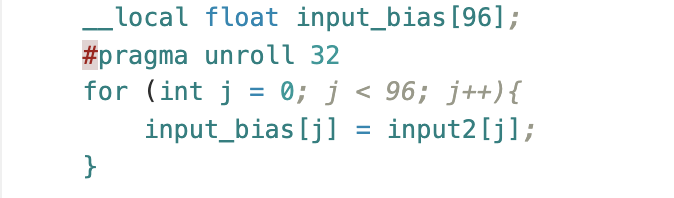
\includegraphics[width=\textwidth,height=\textheight,keepaspectratio]{img/Loop_unrolling.png}
    \caption{Loop unrolling}
    \label{Loop unrolling}
\end{figure}
<\newpage>
\subsection{Pipelining}
Pipelining enables pipeline parallelism. Basically without pipelining, each instruction is processed from start to finish before moving on to the next. But Pipelining allows the various hardware sections to each process a different instruction simultaneously.
\begin{figure}[h!]
    \centering
    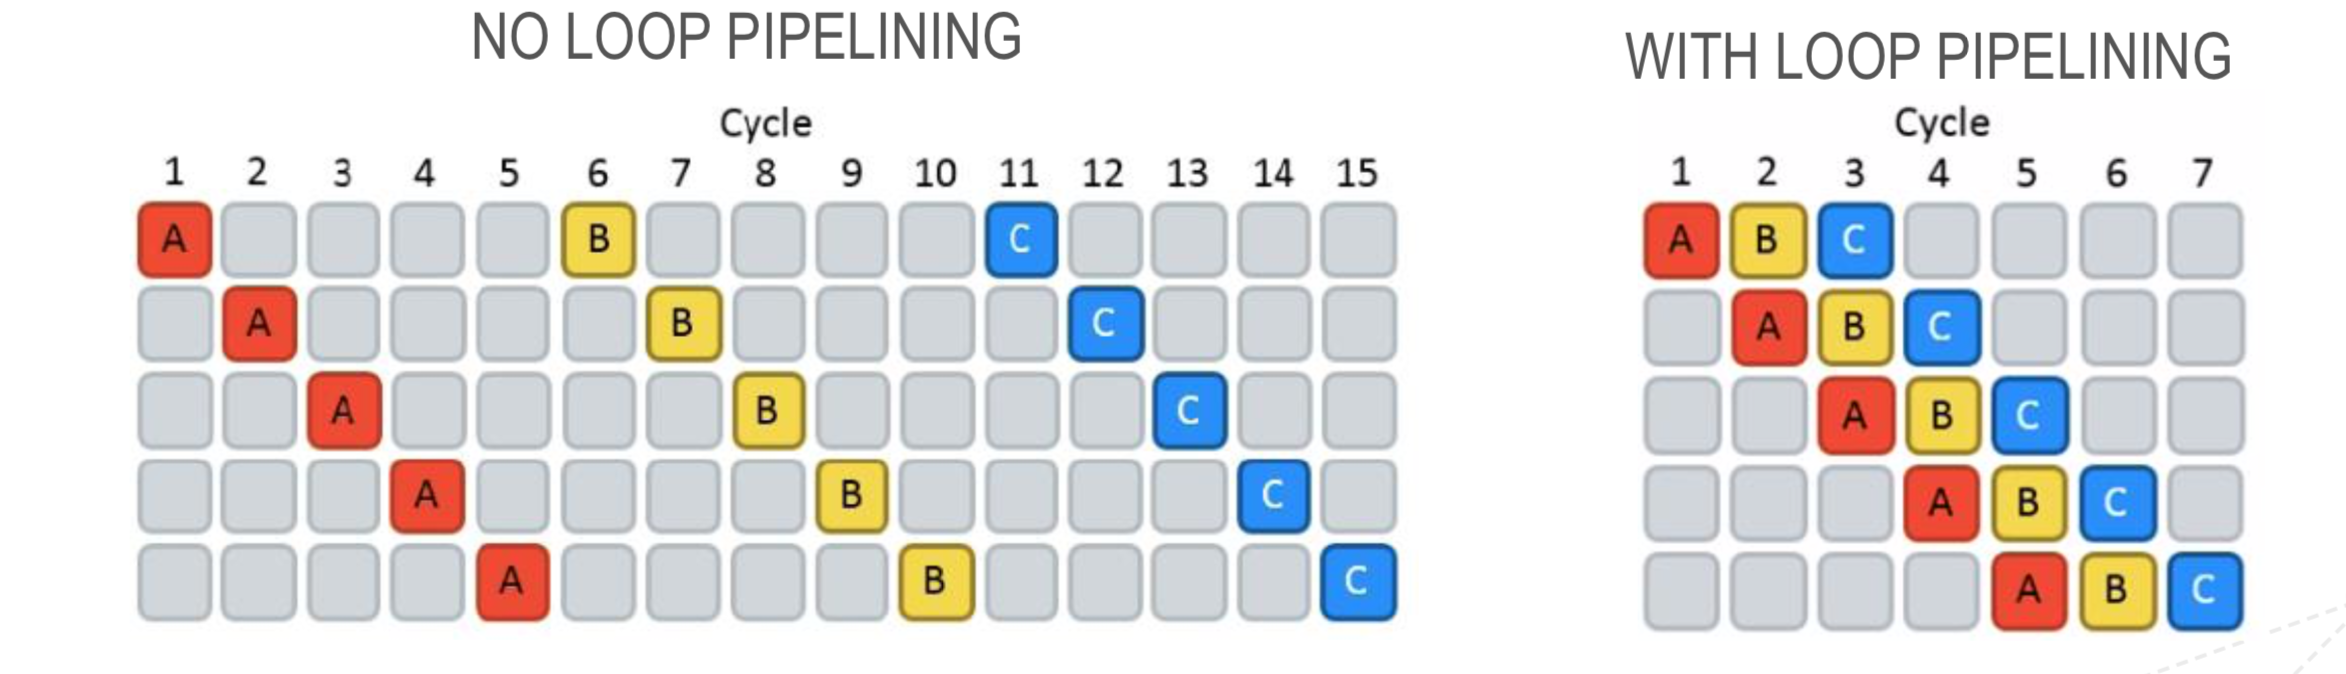
\includegraphics[scale=0.4]{img/Pipelining.png}
    \caption{Pipelining}
\end{figure} 	%includes -tex file with the chapter "Introduction"
\chapter{Goals}
Convolution Neural Network (CNN) is a type of Deep Neural Network (DNN) used in the field of image processing and image analyzing. CNNs are artificial neural network that have so far been popularly used for analyzing images. The role of the CNNs are to reduce the images into a form such that it is easier to process, without losing features which are critical for getting a good prediction. The objective of CNN is to extract features from the input images. 
The main focus of our project is to implement the state-of-the-art CNNs on the FPGAs which acts as an accelerator for compute-heavy neural networks. We have the following sub-goals:
\section{Scaling over multiple FPGAs}
An FPGA is made up of finite and limited resources and implementing these large CNN models can often result in running out of resources and cannot fit into a single FPGA. Hence in this project, we have used the FPGA infrastructure in the Noctua cluster. The Noctua cluster is a high-performance computing system equipped with 32 Intel Stratix 10 FPGAs with point to point connections. We have also scaled our CNN models on the Noctua cluster by partitioning the large model into smaller models based on the number of layers that will fit onto a single FPGA and these smaller models were executed on multiple FPGAs to provide low latency computation. We have used the OpenCL external I/O channels to transfer intermediate results from one FPGA to another. By scaling our application on multiple FPGAs infrastructure we target to perform as good as the Microsoft's Project Brainwave architecture in terms of latency and throughput.
\par
Microsoft Project Brainwave is a deep learning platform for real-time Artificial Intelligence (AI) applications like computer vision. Brainwave is equipped with Intel Stratix 10 FPGAs in the Microsoft Azure Cloud and Neural Processing Units (NPU) architecture for executing a DNN model with low latency and high throughput. Brainwave also supports multiple FPGAs infrastructure in the Azure cloud. When the memory resource of the FPGA is exhausted by the DNN model layers, the remaining layers will be mapped to the next FPGA enabling scaling.

\section{Performance Optimization}
Heterogeneous computing systems provide performance gain by using specialized capabilities of different types of processors (CPU+FPGA in our project). OpenCL is a framework for heterogeneous computing which provides software-centric development flow for FPGAs and obtains performance and power advantages with hardware acceleration. We have used the OpenCL tool flow for developing CNN models in our project inorder to develop individual kernels for each layer of the CNN model. Also, we considered the concept of channels offered by OpenCL to transfer intermediate results from one layer to the next layer without writing the results in the global memory. The kernels were further optimized by using several OpenCL optimization techniques learnt during the tutorial phase eg: loop unrolling, reducing the Initiation Interval (II) of loops to 1, removing memory dependencies, etc. Performance modeling was applied to each OpenCL kernels to identify the bottlenecks in the design and resolve the issues to obtain  high throughput and high utilization.

\section{Quantization }
CNN implementation is often complex due to the large number of parameters and computations, which makes it difficult to be implemented on a resource constrained FPGA. The floating point operations are computationally expensive, hence quantization can be applied to the deep networks to convert the floating point weights into fixed point weights. Fixed point operations typically consumes fewer hardware resources than floating point operations. Quantization will help in reducing the power consumption, memory footprint and resources utilization. In our project, we rely on Intel OpenVINO to optimize and quantize the CNN model so that the accuracy is not drastically dropped in the quantized model. We will also distinguish the models with quantized weights and floating point weights.
		%includes -tex file with the Goals
\chapter{Metrics} \label{chp:Metrics}
Our objective was to leverage the infrastructure available at the Paderborn Centre for Parallel Computing (PC2) to build an inference accelerator system. We evaluated the effectiveness of our inference accelerator system by considering two classes of metrics - performance metrics and quality metrics.  

Performance metrics just account for the arithmetic operations performed on the FPGA. They do not tell whether the operations being performed are functionally correct or not. To account for the quality of the operations being performed, we considered accuracy, which is defined a little further down in this chapter. As we have used existing, pre-trained network topologies, we aimed to attain (or reach as close as possible to)  the accuracy mentioned in the literature.

\section{Performance Metrics}

\subsection{Operations per cycle}
Operations per cycle is a unit of measure for the numerical computing performance of a computer. Typically expressed as OPs/cycle, this metric tells us how many operations are performed in one clock cycle of the targeted hardware.  

To calculate OPs/cycle we looked at the source code and the final profiler report from the executed code. From the source code, we calculated the number of operations sans the overheads (loop index calculations, loop increment operations, etc). From the profiler report, we got a concrete number for the clock frequency of the FPGA and the execution time. Combining these two allowed us to calculate operations per cycle.

\subsection{Operations per second}
Operations per second is closely related with the above metric “Operations per cycle”. It is usually expressed as OPs/second. OPs/second depends on the clock frequency of the platform. 
We calculated “operations per second” by simply dividing the number of operations by the execution time.  
As per literature mentioned in Chapter 7 named Related Work, popular tool-flows like DNNWEAVER on Arria 10 GX115 have achieved 184.33GOPs/second, running at a clock frequency of 200MHz.

\subsection{Operations per byte}
Operations per byte or Arithmetic Intensity is the number of operations performed per byte of data transferred between the FPGA and off-chip memory.  
In our case, we calculated the number of operations performed and the total amount of data transferred by looking at the source code. We also looked at the profiler report at the end of execution to get the correct estimation of data transferred between global memory and local memory.  
This metric helped us to identify if we are memory bandwidth limited or compute resource-bounded.  

The metrics OPs/second and OPs/byte made up the metrics required to do Roofline Analysis of our inference system.  


\subsection{Latency}
Latency is generally defined as the time delay between initial input to a system and the output from the system. Latency captures the time it takes to load data, pre-process it, send said data over a network to the Inference Engine, the time needed for inference, and time needed to send the classified data back to the user. 

In our case, the focus was on improving the time needed for inference and hence we redefined latency to refer to only the amount of time to infer an image on FPGAs ( i.e, without considering the overheads).

Latency can be measured for just a single image or over a batch of images. We can expect to have different latencies based on how we measure it (single image vs batch of images). As an example of what has been achieved in related works, we have ALAMO tool-flow running on Arria 10 GT115 running at 239.62MHz having a latency of 4.05ms.
We aimed to have latency in this range.

\subsection{Throughput}
Throughput is a measure of the amount of information processed per unit time. In our case, we defined it as the number of images classified per second. There are well-known techniques to improve throughput like batch processing where a number of images are batched together and sent for inference job. 
But as the batch size goes up, latency also tends to go up. So there is a trade-off involved here between throughput and latency.  \par
We had deployed a pre-trained ResNet-50 DNN model in the Microsoft Azure cloud during our research phase and the images were classified in less than 4 ms and a maximum throughput of 39.5 Teraflops on a single Stratix 10 FPGA. Hence, we decided to benchmark our project group's implementation against Microsoft Project Brainwave.



\section{Quality Metrics}
\subsection{Accuracy}
Accuracy is defined as the fraction of the number of correct inferences made to the total number of inferences made. In our context, accuracy depended on the CNN topology used, nature of weights (floating point vs fixed points, etc), training data, etc. 
In literature, accuracy is expressed in terms of percentages and the changes from baseline model's accuracy is measured in terms of percentage points (pp). 
In our case, baseline models were the existing, trained topologies mentioned in Chapter \ref{chp:DataTopoArch}. Our goal was to make use of DNN approximation techniques and still achieve accuracy within 3pp of the baseline model.
\newline
Since we made use of pre-trained models in this project, there was no change in accuracy of classification given by our Inference Engine.
To check the accuracy of the label and score given by the Inference Engine, the pre-trained models were executed in TensorFlow and output for the same were retrieved. If the output score of the Inference Engine was same as that given by TensorFlow then the classification was deemed accurate else changes had to be made to output the correct score.

\subsection{Rate Correct Score}
Taking inspiration from the field of Memory and Cognitive research, we combined accuracy and latency by considering Rate Correct Score. It is defined as 

\begin{equation} \label{eqt:example_equation}
RCS = \frac{c}{\sum R_t}
\end{equation}
\equations{Rate Correct Score}

%$RCS = \frac{c}{\sum R_t}$    

where   

$c$ = accuracy    

      $\sum R_t$ = batch execution time  
      
We aimed at maximizing RCS throughout the entire runtime of the project (either by increasing the accuracy or by decreasing the latency or both).
		%includes -tex file with the Metrics
\chapter{Datasets, Topologies and Architecture comparison}\label{chp:DataTopoArch}

\section{Datasets}
CNNs are trained on datasets. Each dataset consists of specific type of images and each of them are used in different tasks such as image classification or image captioning. We decided to use ImageNet as our primary dataset for the project.

\subsection{ImageNet}
It is one of the most prominent datasets used in the field of visual object recognition. In 2009 this dataset was first introduced to the world in the Conference on Computer Vision and Pattern Recognition by the Computer Science department of  Princeton University. It has over 14 million images and over 20,000 categories. A large portion of the images has been hand annotated which is helpful in the task of image captioning. Every year ImageNet runs a challenge called the ImageNet Large Scale Visual Recognition Challenge (ILSVRC), where different software architectures and algorithms take part in order to classify images of the dataset correctly. By 2017 most of the algorithms working on ImageNet have already achieved accuracy of more than 95\%.


\subsection{ Reasons for Selection of ImageNet Dataset}
Reasons for selecting ImageNet are as follows:
\begin{itemize}
    \item The topologies that were used in the project are well optimized for ImageNet. 
    \item ImageNet provides a greater challenge and the topologies that were used were trained on ImageNet dataset. Hence their results were  used for benchmarking performance.
\end{itemize}
\section{Topologies}
In this section we describe the CNN topologies that were deployed in our project. ResNet-50 and GoogLeNet are some of the state-of-the-art topologies that have performed exceptionally well on the ImageNet challenge. Due to this, we decided to deploy these topologies and investigate how their performance can be improved through FPGA acceleration while maintaining the classification accuracy. The following sections give a detailed explanation about their architectures and basic working principles.

\subsection{GoogLeNet}\label{GoogLeNet_Topo}
GoogLeNet is a deep convolutional neural network and is also known as Inception-V1. It is also a winner of the ILSVRC 2014 in image classification. The architecture is based on the Hebbian principle which states that \textit{cells that fire together wire together} with the intuition of multi-scale  processing\cite{DBLP:journals/corr/SzegedyLJSRAEVR14}. GoogLeNet, shown in Figure \ref{fig:GoogLeNetTopo}, is a 22 layer deep network and it is used for object detection and classification. It has modules known as "Inception modules" - network within a network. This is depicted in Figure \ref{fig:InceptionModule}. GoogLeNet does not have any fully connected layers but uses global average pooling which keeps the model from overfitting the data. It was able to achieve a top-5 error rate of 6.67\% and requires only 4 million parameters, in comparison to this AlexNet requires up to 60 million parameters.

\begin{figure}[!h]
    \centering
    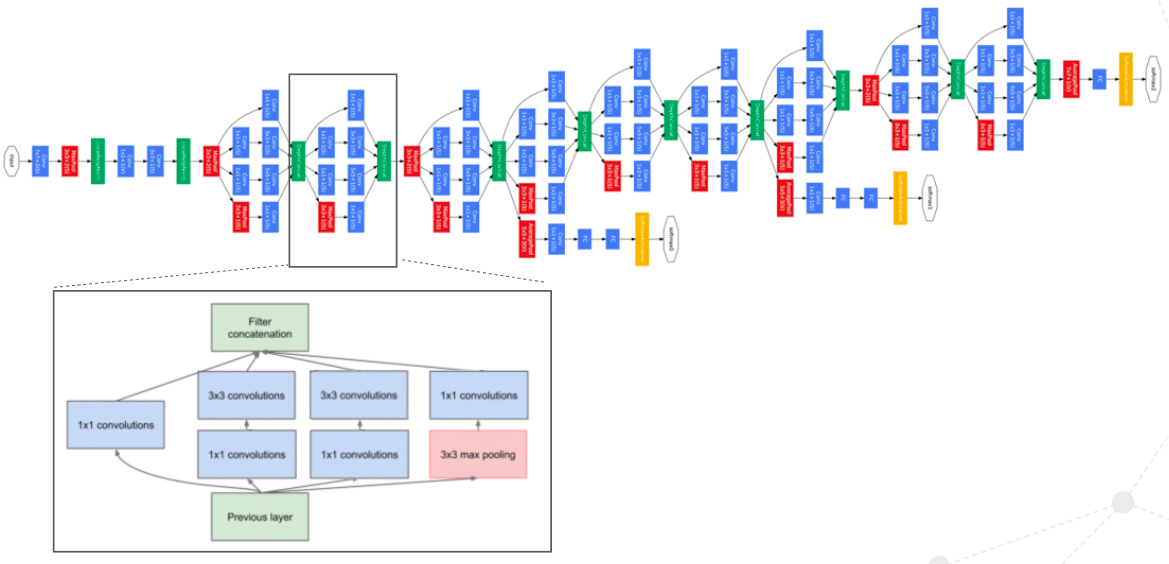
\includegraphics[scale=0.4]{img/googlenetarch.png}
    \caption{GoogleNet Architecture \cite{DBLP:journals/corr/SzegedyLJSRAEVR14}}
    \label{fig:GoogLeNetTopo}
\end{figure}

\subsubsection{Inception Module}
The logic behind Inception architecture is built on finding optimal local sparse structure in the convolution network and to repeat it spatially. There are 9 inception modules in GoogLeNet. Each inception module has 6 convolution layers and 1 max pooling layer spread across 4 branches within the inception module. Some convolution layers and max pool layer are stacked on each other (branch 3) due to which four different outputs are created within the inception module which is concatenated to produce one single output. This output is then passed onto the next inception module and so forth. Concatenation of this output filter occurs based on depth. The 1x1 convolution layers in inception module help us to preserve spatial dimensions and to reduce the feature depth \cite{DBLP:journals/corr/SzegedyLJSRAEVR14}.

The output from the last inception module is forwarded to global average pooling.

\begin{figure}[h!]
    \centering
    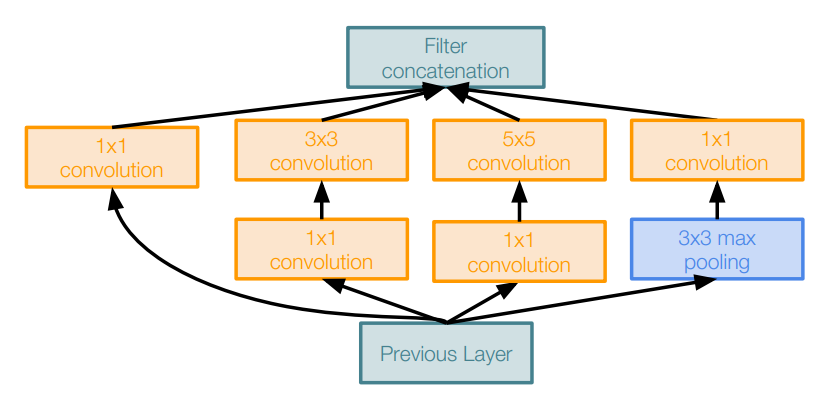
\includegraphics[scale=0.4]{googlenet}
    \caption{Inception Module \cite{DBLP:journals/corr/SzegedyLJSRAEVR14}}
    \label{fig:InceptionModule}
\end{figure}

\subsection{ResNet-50}
ResNet is a deep neural network released by Microsoft and, also a winner of the ILSVRC 2015 in image classification, detection, and localization. ResNet is a series of DNN with different number of layers from 18 to 152. In this project, we implemented a smaller version of  ResNet - called ResNet-50. It has 50 layers. It is shown in Figure \ref{fig:resnet_50}.

The ResNet-50 architecture is divided into 4 blocks. These 4 blocks comprise of 16 units. The units in the blocks are combined based on the depth, i.e, all the units in the block have the same depth. The units of the ResNet-50 consist of 2 1 $\times$ 1 convolution kernels and 1 3 $\times$ 3 convolution kernel. Similar to concat layer in GoogleNet, here we have Eltwise layer which performs element wise addition and generates the output. This output is then fed as an input to the next unit. ResNet uses a special type of connection called as skip connection.  

\begin{figure}[!htb]
\centering
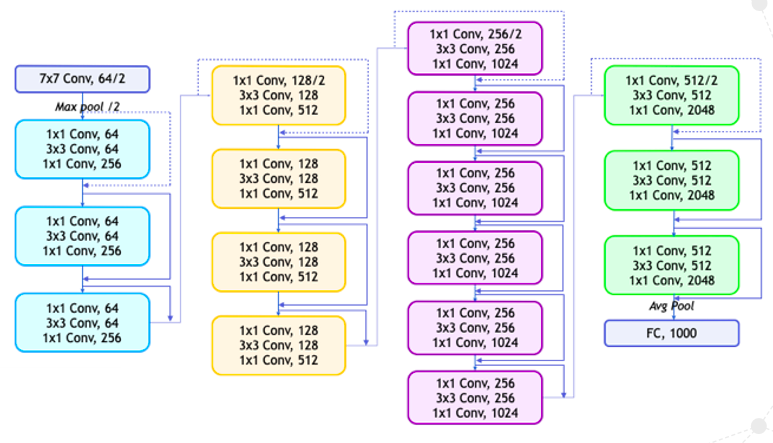
\includegraphics[scale=0.5]{img/Resne50arch.png}
\caption{ResNet-50 \cite{resnet_fig}}
\label{fig:resnet_50}
\end{figure}

\subsubsection{Skip Connections}
The base idea is applying the residual connections which are described as learning the residual representation of functions instead of signal representation. One of the conceptual ideas of ResNet is using the skip connection, as shown in Figure \ref{fig:Skip_connection}. Skip connection makes the network deeper.

Many convolution DNNs run into a problem with vanishing or exploding gradients because, during backpropagation, we derive error function with respect to the current weight and get multiplying of small or large numbers \cite{skip_fig}. The product of small numbers will be zero (vanished) and the product of large numbers will be too large (exploded). Developers of ResNet solved this problem by using a skip connection. In the skip connections for the next layer, they use the input from the previous layer without any modifications. 

The output of skip connection is  F(x) + x and the weight layers actually are to learn a kind of residual mapping: output minus identity x. If we have a vanishing gradient we always have an identity x to send it back to previous layers. 

After each convolution layer, ResNet uses the batch normalization from Inception-v2. 

\begin{figure}[h!]
    \centering
    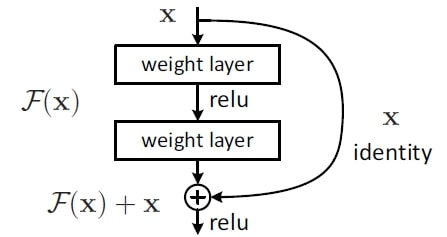
\includegraphics[scale=0.4]{resnet_1}
    \caption{Skip connection \cite{skip_fig}}
    \label{fig:Skip_connection}
\end{figure}

The main concepts of constructing ResNet:
\begin{itemize}
\item Avoiding representational bottlenecks by not abruptly reducing the dimension of data, but smoothly from the beginning of the network to the classifier at the output.
\item Factorization of convolution layer into smaller pieces because this will save resources and help to increase the count of layers.
\item Supporting a balance between the depth and width of the network. One should increase or decrease both dimensions.
\end{itemize}



		%includes -tex file with the chapter "Datasets_and_Topologies"
\chapter{Introduction to Machine Learning Toolkits}
\label{chp:Toolkits}
We have used two state-of-the-art machine learning toolkits in our project, to help us achieve our goals. These tools are:-
\begin{itemize}
    \item Intel OpenVINO computer vision toolkit
    \item Tensor Virtual Machine (TVM)
\end{itemize}
Both these tools have the same high level goal, that being the deployment of pre-trained CNN models on different hardware platforms such as CPU, GPU, FPGA etc. thereby making the high level deep learning frameworks such as Tensorflow, Caffe etc. independent of the underlying hardware. However, none of these tools alone can achieve our goals, making it necessary to use a combination of both, using certain components and features in each toolkit. Both Intel OpenVINO and TVM are described in detail in the next sections.  

\section{Intel OpenVINO}


Intel OpenVINO is an open source toolkit from Intel that allows the deployment of pre-trained deep neural networks on different hardware platforms such as CPU, GPU, FPGA, etc. The toolkit is available for installation for the Windows operating system as well as selected Linux distributions. All of the tool's libraries and plugins except the FPGA plugin are a part of the open source GitHub repository.
The functionality of OpenVINO is divided among its components, Model Optimizer and Inference Engine. This is shown in Figure \ref{fig:OpenVINO_workflow} and explained below. 
\begin{figure}[!hbpt]
    \centering
    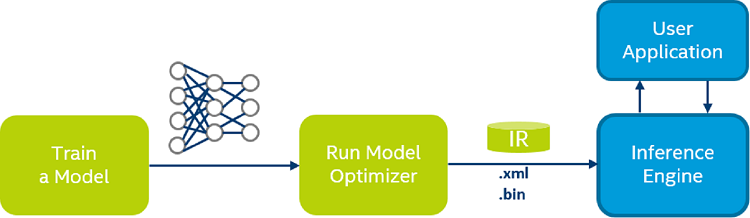
\includegraphics[width=0.65\textwidth]{img/openVINO_workflow.png}
    \caption{Intel OpenVINO workflow \citep[][]{openvino_fig}}
    \label{fig:OpenVINO_workflow}
\end{figure} 

\subsection{Model Optimizer}
The Model Optimizer is a python based tool which takes as input a pre-trained model. It supports many popular deep learning frameworks such as TensorFlow, Caffe, PyTorch, MXnet, etc. This model is then converted to a common intermediate format (IR), thereby making the inference engine independent of the training framework. The IR contains a .xml file which represents the computational graph of the CNN and a .bin file containing the weights. The graph is optimized by fusing different layers of the original topology wherever possible. Typically the batch normalization layers are fused with their preceding convolution layer and the convolution filter weights are accordingly adjusted. The toolkit comes with a model downloader which can download various openly available pre-trained models for different frameworks.
 

 \subsection{Inference Engine}
 The Inference Engine is responsible for the execution of the model on the selected hardware. For this purpose, it provides a C++ API which can be integrated into an application. The main task performed by the inference engine is to read the intermediate representation of the model, select the hardware for deployments such as CPU or FPGA and call the appropriate plugin which defines all necessary data structures and functions required to perform inference and return the output along with performance statistics. 
 The toolkit comes with pre-compiled bitstreams for a few supported FPGA boards. These bitstreams implement various popular network topologies such as GoogLeNet, ResNet, etc. as well as generic layers which are used to program the FPGAs as per the requirement of the given model topology.
 
 These bitstreams however, do not support the Intel Stratix 10 FPGA boards available in the Noctua infrastructure. In addition to this, the FPGA plugin of the inference engine is not open source, making it infeasible to use OpenVINO as a stand alone tool to achieve our project goals without customizing its components at the source code level.
 
 \subsection{OpenVINO source code}
 The Intel OpenVINO toolkit is open source and the code is available as a Github repository known as Deep Learning Deployment Toolkit (DLDT). The repository contains source code for both the Model Optimizer as well as the Inference Engine except for the FPGA plugin. As a result, we have written our own FPGA plugin for OpenVINO to support the Noctua infrastructure and enable scaling of CNNs over multiple FPGAs. 
 
 \subsection{FPGA plugin}
 The main purpose of the FPGA plugin is to flash the bitstreams (.aocx files) for the CNN models on the FPGAs and to launch the kernels according to the CNN topology. It also supports scaling on multiple FPGAs which has been achieved through the use of MPI (Message Passing Interface) and the serial I/O channels present between FPGA nodes in the Noctua infrastructure. 
 
 The plugin interacts with the Inference Engine C++ API which helps in parsing the intermediate representation obtained from the model optimizer for a given CNN model. We have reused the classes and data structures in this API as much as possible, specifically for parsing the .xml file in the IR containing the topology for the given CNN model, parsing the weights in the binary (.bin) file as well as parsing the input images. We have stored all the parsed information from the IR in a C++ struct for each layers. The definition of the struct is shown in the code snippet Code \ref{code:struct}.
 \begin{code}[!htb]
 \begin{minted}{c++}
 /**
 * Data structure to store information of each layer
 */
struct layersDetails
{
	//Layer ID
	int layerID;
	// Layer Name
	std::string layerName;
	//Type of Layer
	std::string layerType;
	//Pointer to the Layer Bias vector
	float *layerBias;
	//Pointer to the Layer Weights vector
	float *layerWeights;
	//Total number of biases
	int num_biases;
	//Total number of weights
	int num_weights;

	//Hashmap for parameters ( kernel, padding,dilation,precision) with its values.
	std::map<std::string, std::string> params;
	//Vector of parent layers
	std::vector<std::string> inputLayerNames;
	//Vector of child layers
	std::vector<std::string> outputLayerNames;
	//Vector of pointers to the Layers Details Structure of Children nodes
	std::vector<struct layersDetails *> children;
	//Vector of pointers to the Layers Details Structure of parent nodes
	std::vector<struct layersDetails *> parents;

	// Buffer index of the output
	int layerOutBufferIndex = 0;
	// vector of buffer index
	std::vector<int> parentOutBufferIndex;
	// Output dimension
	int outH = 0, outW = 0, outDepth = 0;
	//Flag to check if layer is executed.
	int visited = 0;
};

    
\end{minted}
\caption{Struct to store parsed IR information for each layer in CNN}
\label{code:struct}
\end{code}
 
 In addition to this pre-existing source code, we have written our own tree data structure in the plugin, to represent the CNN topology in a suitable pointer structure that adequately models the input output relationships between CNN layers, thus allowing us to launch their corresponding OpenCL kernels in an orderly fashion. 
 
 The plugin also supports scaling over multiple FPGAs, through the use of MPI and dedicated serial I/O connections between FPGA boards that are present in the Noctua infrastructure. The infrastructure consists of 16 FPGA nodes, each hosting 2 Intel Stratix 10 FPGA boards. Our plugin has multiple instances running as MPI processes, one per node. Each plugin instance is thus responsible for the execution of partial CNN topology on 2 FPGAs. We divide the CNN model at the OpenCL level into multiple .cl files which are then synthesized to generate their corresponding bitstreams. These bitstreams are then named in a suitable fashion so as to create a mapping between them and the specific plugin instance running on a FPGA node which is identified by its MPI rank. To map the names of the CNN layers (OpenCL kernels) to the .aocx file that contains them, we use Intel OpenCL SDK binutils to generate a .xml file corresponding to each .aocx bitstream. The plugin instance would thus flash appropriate .aocx files according to its MPI rank and then launch appropriate kernels that are contained in those .aocx files, after parsing the corresponding xmls. 
 
 The sequence diagram in the Figure \ref{fig:plugin_uml} shows the operations during the execution of the plugin.
 \begin{figure}[!hbpt]
    \centering
    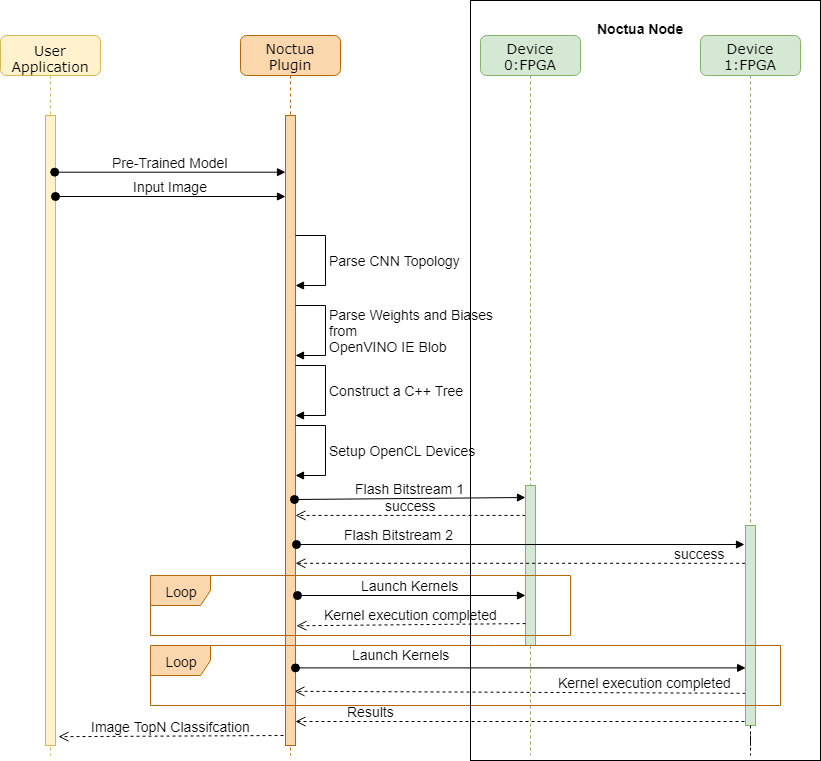
\includegraphics[width=\textwidth]{img/Plugin_UML_1.png}
    \caption{Sequence diagram of the Inference Engine at one node}
    \label{fig:plugin_uml}
\end{figure} 

 \begin{itemize}
     \item The user application sends the CNN model IR and the input image to the plugin.
     \item The FPGA plugin parses the IR, both the xml and bin files to retrieve the layer information and the weights which are then used to construct a tree data structure.
     \item The plugin instance then flashes the appropriate bitstreams on the FPGA boards and parses their corresponding xml files to get a mapping between the aocx files and the kernel names.
     \item The kernels are then launched by a level wise traversal of the tree structure representing the CNN model.
     \item One instance of the plugin is executed parallelly at every node.
     \item The plugin instance at the last node collects results and returns them to the user application which displays the top N labels and their softmax scores (confidence) to the user.
 \end{itemize}
 
 \subsection{Advantages}
  
 \begin{itemize}
 \item Supports optimization of models and quantization of weights.
 \item A CNN model can be deployed on hardware with minimal programming effort and independent of the training framework.
 \item For FPGAs, the use of pre-compiled bitstreams eliminate the time needed for synthesis of kernel codes.
 \end{itemize}
 
 \subsection{Disadvantages}
 \begin{itemize}
 \item The main disadvantage is the compatibility of FPGA boards. Development and synthesis of kernel codes along with a plugin for FPGAs may be required to make OpenVINO work with unsupported boards. 
 \item Scaling to multiple FPGAs, which is one of the goals of this project is non-trivial as it would require the development of overlays for external I/O channels. 
 \end{itemize}
\section{TVM}
Due to extensive research in the field of machine learning especially in Image recognization and object detection largely due to competition such as ILSVRC (Imagenet Large scale visual recognization challenge), there is a demand and need for developing hardware specific to increased computation capabilities and caching mechanisms. Various computational superior hardware such as CPU, GPU, and accelerators such as ASICs and FPGA are been used to deploy Machine Learning (ML) models and to draw the inference. To build and deploy such ML models we use Deep learning (DL) frameworks such as Tensorflow, Caffe, MXNET, Keras, etc. There is extensive support and libraries available for CPUs and certain vendor-specific GPUs. But for accelerators, there is limited support and libraries available which makes it difficult and tedious to deploy ML models on them.  We use Tensor Virtual Machine (TVM) an open-source compiler and code generator which addresses “graph level and operator level optimizations” \cite{tvm_fig}. TVM supports a wide range of hardwares and accelerators. 

There are two types of optimizations that can be carried out during code generation for a DL model, high-level optimizations where graph and operators of the model are optimized and low-level optimizations where low-level programs are  optimized with respect to specific hardware architecture.
Each hardware has its own memory architecture, data operators and dataflow handling mechanism this diversity makes it difficult for efficient graph generation and machine code optimizations.
TVM performs high-level optimizations such as operator fusion where basic operators are fused together and also perform graph optimization where DL activation functions are fused along with convolutions or other functions. It also performs machine code optimizations based on the hardware architecture and compute primitives. TVM uses a learning-based cost model for selection of operators involved in code generation. The TVM compilation stack is shown in Figure \ref{fig:tvm_fig}.

\begin{figure}[h!]
    \centering
    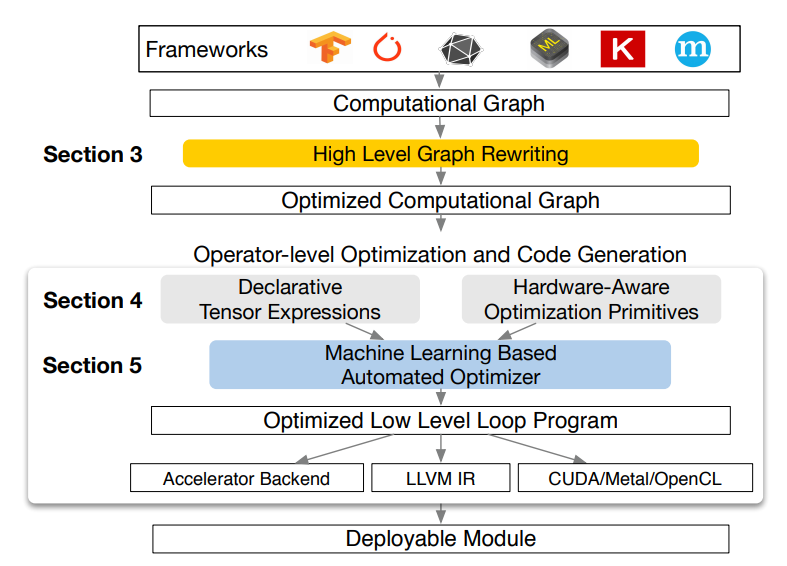
\includegraphics[scale=0.50]{tvm_overview.png}
    \caption{System overview of TVM \cite{tvm_fig}}
    \label{fig:tvm_fig}
\end{figure} 

Following Chen et al.\cite{tvm_fig} TVM performs these three steps: 
\begin{enumerate}
  \item DL frameworks take a model in the form of a frozen \textit{protobuf} file and transform it into a computational graph representation. This computational graph is provided to the TVM graph rewriter which performs graph level optimizations such as operator fusion, constant folding, static memory planning pass, and data layout transformation. These graph level optimizations are been discussed below.
  \begin{itemize}
     \item Operator Fusion - Computation graph intermediate representation (IR) stores intermediate results of certain operators before being used for further computations. TVM performs operator fusion where such operators are fused together along with its predecessor or successor operators based on the type of operator and the operations it performs to form a single kernel. TVM classifies operators into four types namely 1) injective 2) reduction 3) complex-out-fusable and 4) opaque (unfusable operators) \cite{tvm_fig}.
     \item Constant Folding - Certain graph operators have constant values that can be pre-computed during compile time instead of runtime. Thus saving resources and time during code-generation. Constant-folding is a process of finding such operators and replacing them with a constant value. In TVM, it is performed by graph rewriter which mathematically calculates the constant value for such operators and substitutes them in the graph.
     \item Static memory planning pass - Intermediate tensors (data) needs to be stored for further executions. During computational graph optimization, graph rewriter pre-allocates memory to store such tensors.
     \item Data layout transformation - Each hardware has its own data-layout choices based on various factors and memory hierarchies. The computational graph needs to match the internal data layout of the selected hardware. Graph rewriter performs data layout transformation, where it first collects the constraints and ideal data layout for the operators in the selected hardware. These constraints are based on the memory hierarchy of the hardware. Then the mapping of the data layout is performed between the selected operator and the hardware.
   \end{itemize}.
   
  \item TVM has developed \textit{tensor expression language} which provides compute operators with its computing rules and shapes. It supports arithmetic and mathematical operators which are used for computation in DL models. The key feature of this tensor expression is that it is hardware aware language which means based on the target hardware operators can be optimized to gain maximum benefit from the optimization. TVM implements a concept known as “schedule transformation” \cite{tvm_fig} by applying basic transformations on the tensor expressions in a periodic and incremental fashion. During this process, it also keeps additional information about the loop structures and data types which is used during low-level code generation.
  
  TVM implements nested parallelism using the idea of \textit{shared-nothing nested parallelism} and allowing a certain group of threads to fetch data required by them and store it in local memory for easy access. Such collaboration helps in sharing the data with its counterpart/sibling threads. For latency hiding, TVM introduces a concept called “virtual threading schedule primitive” \cite{tvm_fig} where pipeline parallelism is implemented for the target hardware by generating single instruction set from multithreaded instructions which are provided using virtual threads. The single instruction set is achieved using low-level synchronization.
  
  \item  TVM provides us with multiple implementations of the operators, selecting between these operators is based on performance of the operator implementation with respect to the selected hardware. TVM solves this problem by developing a concept called “automated schedule optimizer” \cite{tvm_fig}.
Automated schedule optimizer consists of two components:

\begin{itemize}
     \item Schedule Explorer - Creates a template configuration for the selected hardware with the help of configurable options provided by the developer.
     \item ML-Based Cost model - For the selected operator configuration, the ML model predicts the runtime of the lowered loop program from the configuration. The model training is carried out based on the runtime data collected from various configurations. As more and more configurations are provided the cost model improves its accuracy.
   \end{itemize}
\end{enumerate}


 \begin{code}[!htb]
 \begin{minted}{Python}
target = 'aocl_sw_emu'
target_host = 'llvm'
layout = 'NCHW'
ctx = tvm.cpu(0)

img_path = download_testdata(image_url, img_name, module='data')

model_path='resnet_frozen.pb'

with tf.gfile.FastGFile(model_path, 'rb') as f:
    graph_def = tf.GraphDef()
    graph_def.ParseFromString(f.read())
    graph = tf.import_graph_def(graph_def, name='')
    graph_def = tf_testing.ProcessGraphDefParam(graph_def)
    # Add shapes to the graph.
    with tf.Session() as sess:
        graph_def = tf_testing.AddShapesToGraphDef(sess,
        'resnet_v2_50/predictions/Reshape_1')   

from PIL import Image
image = Image.open(img_path).resize((224, 224))

shape_dict = {'DecodeJpeg/contents': x.shape}
dtype_dict = {'DecodeJpeg/contents': 'uint8'}

sym, params = nnvm.frontend.from_tensorflow(graph_def, layout=layout,
shape=shape_dict)


with nnvm.compiler.build_config(opt_level=3):
    graph, lib, params = nnvm.compiler.build(sym,  target=target,
    target_host=target_host,  params=params)


\end{minted}
\caption{TVM Python API code for ResNet-50}
\label{code:TVMAPI}
\end{code}


In Code \ref{code:TVMAPI}, we use TVM API to get OpenCL generated code for ResNet-50 model.
After the compilation of the program, TVM provides us with an output file with the kernels for FPGA, the optimized computation graph, the library of operators present in the graph for the target hardware (FPGA) and the parameters which contain weights and input for the model. The computational graph also provides us with intermediate representation and mapping of the code generated with its respective inputs.

\pagebreak
 
 Following are the important components of TVM.
 
 \subsection{Compilers}
 TVM provides us two types of compilers.
 
 
 \subsubsection{NNVM}
 
 Neural Network Virtual Machine (NNVM) is a compiler that implements operator and graph level optimizations provided by TVM to generate target hardware code. \textit{nnvm.top} (Tensor operator property registry) provides information about which operators can be scheduled together and performs those optimizations to produce the optimized graph.
 
 NNVM has four levels of operators :
 
 \begin{itemize}
    \item Level 1: Basic Operators - This level includes vary basic operators such as \textit{dense}, \textit{Relu}, \textit{sigmoid}, \textit{exp}, etc.
    \item Level 2: Convolutions - The operators related to convolution become part of this level. Eg. \textit{con2d}, \textit{max\_pool2d}, \textit{avg$textunderscore$pool2d}, etc.
    \item Level 3: Additional Tensor Operators - Operations that provide the additive feature to the original tensors are group together at this level. Eg- \textit{reshape}, \textit{floor}, \textit{round}, etc.
    \item Level 4: Broadcast and reductions - Operators such as \textit{sum}, \textit{mean}, \textit{max},  \textit{min} are part of the reduction level.
 \end{itemize}
 
 NNVM has following functionality:
 
 \begin{itemize}
    \item \textit{nnvm.frontend} take in the model provided by DL frameworks and generates NNVM compatible symbols and parameters (NDArray) which are used by NNVM.
    \item  \textit{nnvm.compiler} has  \textit{nnvm.build} and  \textit{nnvm.build\_config} functions.
    \item In \textit{build\_config} function we provide optimization level based on which graph and tensor optimizations are carried out.
    \item \textit{nnvm.build} function is used to make C API call for code generation with optimized computational graph (graph), target hardware (targer\_host), input parameters (param) and layout provided. 

 \end{itemize}
 
 TVM provides us with the following types of optimizations.
 
 \begin{itemize}
     \item Pass 0 \textit{SimplifyInference} -
It is usually carried out on batch normalization tensor operators.
 \item Pass 1 \textit{OpFusion} -
In \textit{OpFusion}, basic operators are fused together with the convolution layer along with the precomputation of tensor operators.
\item Pass  2 \textit{PrecomputePrune} -
In this level of optimization, the graph is pruned and the constant operators are precomputed and replaced with constant values. The values of such operators are mathematically precalculated and substituted with a constant value during kernel generation. The number of operations is reduced in a precomputed and pruned graph.
\item Pass  3 \textit{FoldScaleAxis} -
In \textit{FoldScaleAxis} algorithm, "[t]he general idea is to transform [tensor expression] to a tuple of value, axes, and scale, where the
final result satisfies [code \ref{code:TVMFoldScaleAxis}].
\begin{code}[!htb]
 \begin{minted}{Python}

 result = value
 for i, k in enumerate(axes):
    k-th dimension of result *= i-th dimension of scale
 \end{minted}
 \caption{TVM FoldScaleAxis \cite{FoldScaleAxis}}
\label{code:TVMFoldScaleAxis}
\end{code}
Then [compiler] can propagate this signal [tuple] along and fold the scale if necessary. [. . .] In order to make sure all the scale [compiler] sent out can be consumed eventually, [compiler runs] a backward 'preparation phase', which propagates the demand of the potential axes scaling back to its input" \cite{FoldScaleAxis}.
We have used this optimization level during our kernel generation.
 \end{itemize}
 
  \subsubsection{Relay}
Relay is known as NNVM {$V_2$}. It is a high-level functional IR for TVM.  Relay has 8 levels of definitions and is finely grained with extended support of \textit{Image operators}, \textit{Algorithm operators}, \textit{Temporary operators}, and \textit{dialect operators}. It distinguished between local and global variables been used.

\begin{itemize}
    \item Relay uses similar levels of optimizations as NNVM.
    \item \textit{relay.backend}  handles the backend request for relay interpreters. Various relay functions can be accessed through the \textit{relay.backend} interpreter.
    \item \textit{relay.frontend},  \textit{relay.build}  and \textit{relay.build\_config}  has similar functionality to its predecessor.
\end{itemize}

 \subsection{TOPI}
 For having quick access to the operators, TVM creates a library of its operators naming TVM Operator Inventory (TOPI). It contains a list of predefined operators that are used to compute operator declaration while generating computational graph. List of operators supported by TOPI are \textit{identity}, \textit{negative}, \textit{floor}, \textit{ceil}, \textit{abs}, etc.
 \begin{itemize}
\item \textit{topi.identity(x)} Returns with the identity value for the selected input.
\item \textit{topi.negative(x)} Returns with the negative value for the selected input.
\item \textit{topi.abs(x)}  Returns element-wise absolute value for the tensor operators.
 \end{itemize}
 
 \subsection{Codegen}
TVM maintains a subdirectory for code generation functionalities and it is placed under \path{src/codegen} and interacts with it using API calls. When we execute \textit{nnvm.compiler.build} function, a C++ API call is made to codegen library which is implemented in C++. When we execute the NNVM compiler an API call is registered under python \path{/tvm/api.py}. The functions present in \textit{api.py} are mapped to   \path{src/api/api_lang.cc} in its C++ counterpart.
 
  \begin{code}[!htb]
 \begin{minted}{c++}
 TVM_REGISTER_API("_Placeholder")
.set_body([](TVMArgs args,  TVMRetValue* ret) {
    *ret = placeholder(args[0],
                       args[1],
                       args[2]);
  });
 \end{minted}
\caption{TVM Register API for Placeholder Operation \cite{tvm_code}} 
\label{code:TVMRegisterAPI}
\end{code} 
In TVM C++ functions are made accessible to Python frontend using \textit{TVM\_REGISTER\_*}. In Code \ref{code:TVMRegisterAPI} a register call made to placeholder operation for Resnet-50 kernel generation.
 
 \begin{code}[!htb]
 \begin{minted}{c++}
 runtime::Module Build(const Array<LoweredFunc>& funcs,
                      const std::string& target) {
  std::string mode = target;
  size_t pos = mode.find(' ');
  if (pos != std::string::npos) {
    mode = mode.substr(0, pos);
  }
  std::string build_f_name = "codegen.build_" + mode;
  // the build function.
  const PackedFunc* bf = runtime::Registry::Get(build_f_name);
  CHECK(bf != nullptr)
      << "Target " << target << " is not enabled";
  runtime::Module m = (*bf)(funcs, target);
  return m;
}
\end{minted}
\caption{TVM codegen Build() function \cite{tvm_code}}
\label{code:TVMCodegen}
\end{code}

 The \textit{Build()} function looks up the code generator for the given target in the \textit{PackedFunc} registry. Code \ref{code:TVMCodegen} shows build function our target library is AOCL. To have a direct interaction between C++ and Python functions a \textit{PackedFunc} is implemented by TVM. Due to interoperability, a Python function can be easily called from C++ codebase making it a bidirectional connection. A \textit{PackedFunc} helps TVM make API calls type-erased, which removes the restriction for the function to be bound to specific input and return from C++ codebase. The inputs provided to the \textit{PackedFunc} are wrapped into \textit{TVMArgs} data type which is an internal data type of TVM and the function returned values are wrapped into \textit{TVMRetValue} data type. In Code \ref{code:TVMCodegenRegisterAPI} \textit{set\_body} is the \textit{PackedFunc} for the API. Since target hardware for our project has been set to aocl, \textit{Build()} function registers \textit{codegen.build\_aocl}.
 
  \begin{code}[!htb]
 \begin{minted}{c++}
  TVM_REGISTER_API("codegen.build_aocl")
.set_body([](TVMArgs args, TVMRetValue* rv) {
    *rv = BuildAOCL(args[0], args[1], false);
  });
\end{minted}
\caption{TVM codegen register API \cite{tvm_code}}
\label{code:TVMCodegenRegisterAPI}
\end{code}

\textit{BuildAOCL()} function generates OpenCL kernels from the lowered IR using \textit{CodeGenAOCL} class. Lowered IR provides us with target hardware IR in the form of machine code which can be used for code generation. The computational graph which is a high-level IR is converted in low-level IR during this process.

 \begin{code}[!htb]
 \begin{minted}{c++}
runtime::Module BuildAOCL(Array<LoweredFunc> funcs, std::string target_str,
                          bool emulation) {
  // Get code.
  using tvm::runtime::Registry;
  bool output_ssa = false;
  CodeGenOpenCL cg;
  cg.Init(output_ssa);
  for (LoweredFunc f : funcs) {
    cg.AddFunction(f);
  }
  std::string code = cg.Finish();
  if (const auto* f = Registry::Get("tvm_callback_opencl_postproc")) {
    code = (*f)(code).operator std::string();
  }

  // Write a .cl file.
  runtime::SaveBinaryToFile("aocl.cl", code.c_str());
\end{minted}
\caption{BuildAOCL() kernel generation \cite{tvm_code}}
\label{code:TVMCodegenBildAOCL}
\end{code}

\textit{BuildAOCL()} function parses through \textit{loweredFunc} and stores the code in \textit{aocl.cl} file. Fig 6.7 shows functionality of \textit{BuildAOCL()}

 \subsection{VTA}
TVM has a DL accelerator for FPGAs and GPUs in the form of Versatile Tensor Accelerator (VTA). VTA is an open-source hardware and can be customized according to the needs and requirements for various DL accelerators. FPGAs support streamlined workflow models, to make deployments of such models fluent VTA provides support for streamlined architecture. Dense linear algebra is one of the important aspects of DL. VTA performs computations such as dense linear algebra using RISC processors thus reducing the execution time and increasing the efficiency at the same. VTA has four modules namely fetch, load, compute and store module. The channel of communication between these modules is through local memory blocks (SRAM) and FIFO queues. Due to the FIFO queues, task parallelism is maintained between these modules.
\begin{itemize}
\item \textit{Fetch Module} – Instruction set needs to be loaded for computation from global memory (DRAM) and also needs to be decoded for routing them to the proper command queue. Fetch module performs those operations on the instruction set.
\item \textit{Load Module} - Once the instruction set is loaded into the module there respective input data and weights need to be loaded from DRAM and are allocated onto on-chip memory.
\item \textit{Compute Module} – Compute module is where all the computations happen for VTA. It uses General Matrix Multiplication (GEMM) to compute dense linear algebra. VTA processors require its data into register file and micro-op kernels into the micro-op cache for further processing, compute module performs those operations of loading of data from DRAM and micro-op kernels.
\item \textit{Store Module} – Stores results from \textit{compute module} into DRAM.
 \end{itemize}
 
 \begin{figure}[h!]
    \centering
    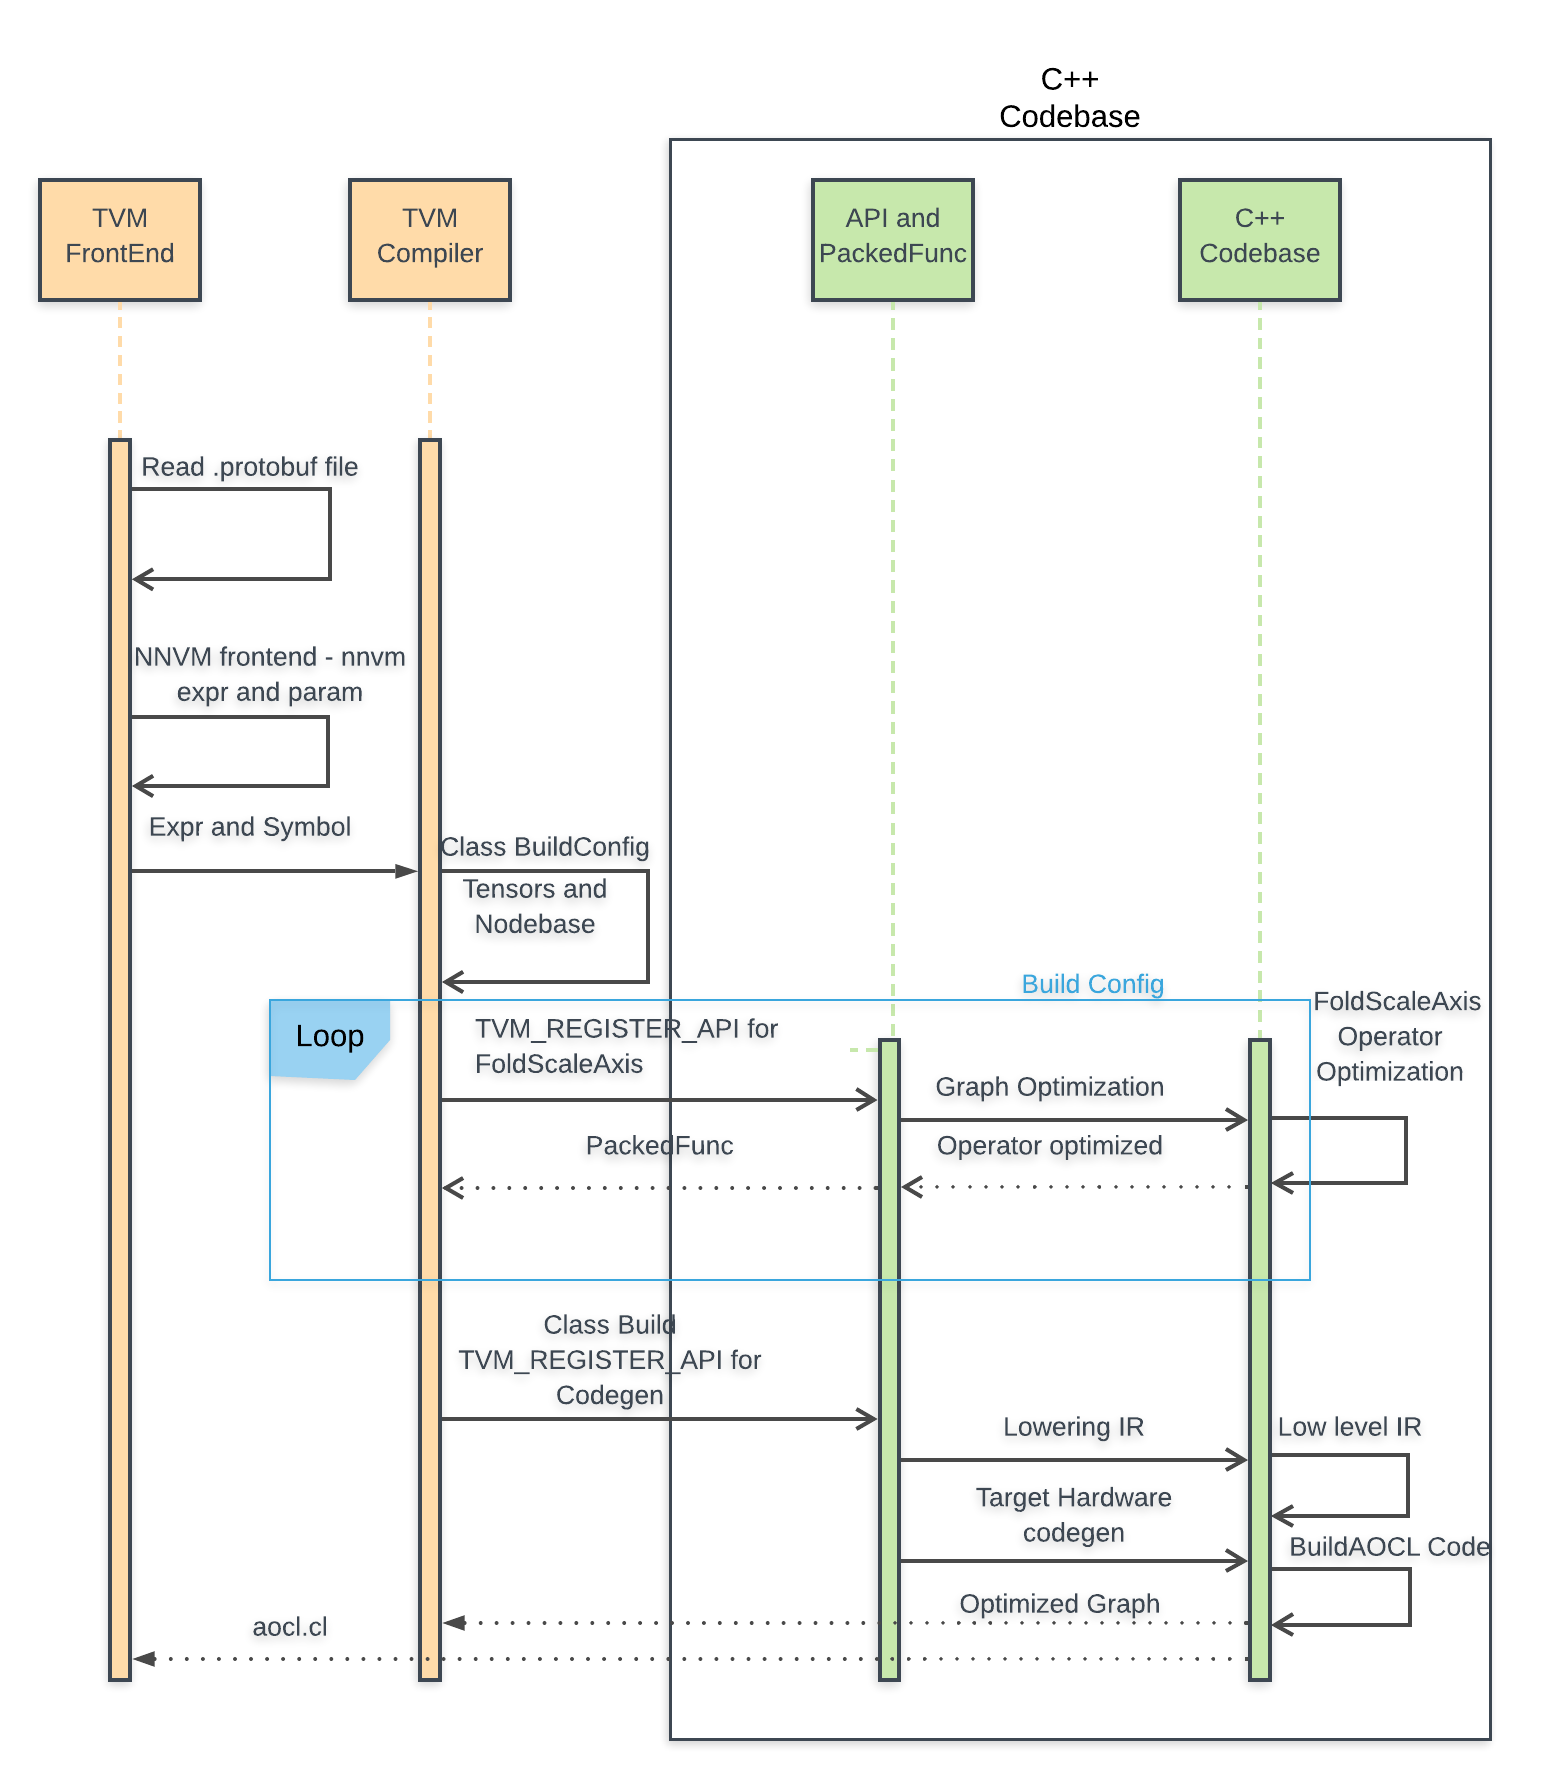
\includegraphics[scale=0.30]{tvm_workflow.png}
    \caption{Sequence diagram of Kernel generation in TVM}
\end{figure}
\pagebreak
 
 \section{Selection of Toolkits}
Reasons for selecting OpenVINO and TVM
 \begin{itemize}
 \item Both Intel OpenVINO and TVM toolkits provide similar features such as Layer fusion, Optimizer, and Quantizer as model optimizer components for optimization of the CNN model. 
 \item We restricted the use of TVM just as OpenCL kernels generator because TVM's AOCL backend for inference was still in experimental phase.
 \item The OpenVINO Inference Engine, as explained earlier comes with several plugins for hardware platforms such as CPU, GPU, FPGA etc. respectively. The FPGA plugin available by default is not open source and works only with certain FPGA boards for which it contains pre-compiled bitstreams. 
 \item Thus, we developed our own FPGA plugin, extending the capabilities of OpenVINO Inference Engine, to make it operational with Stratix 10 FPGAs in the Noctua Cluster of the PC2 infrastructure. 

 \end{itemize}		%includes -tex file with the chapter "Introduction_to_toolkits"
\chapter{Project Architecture}
 \begin{sidewaysfigure}[h!tb]
    \centering
    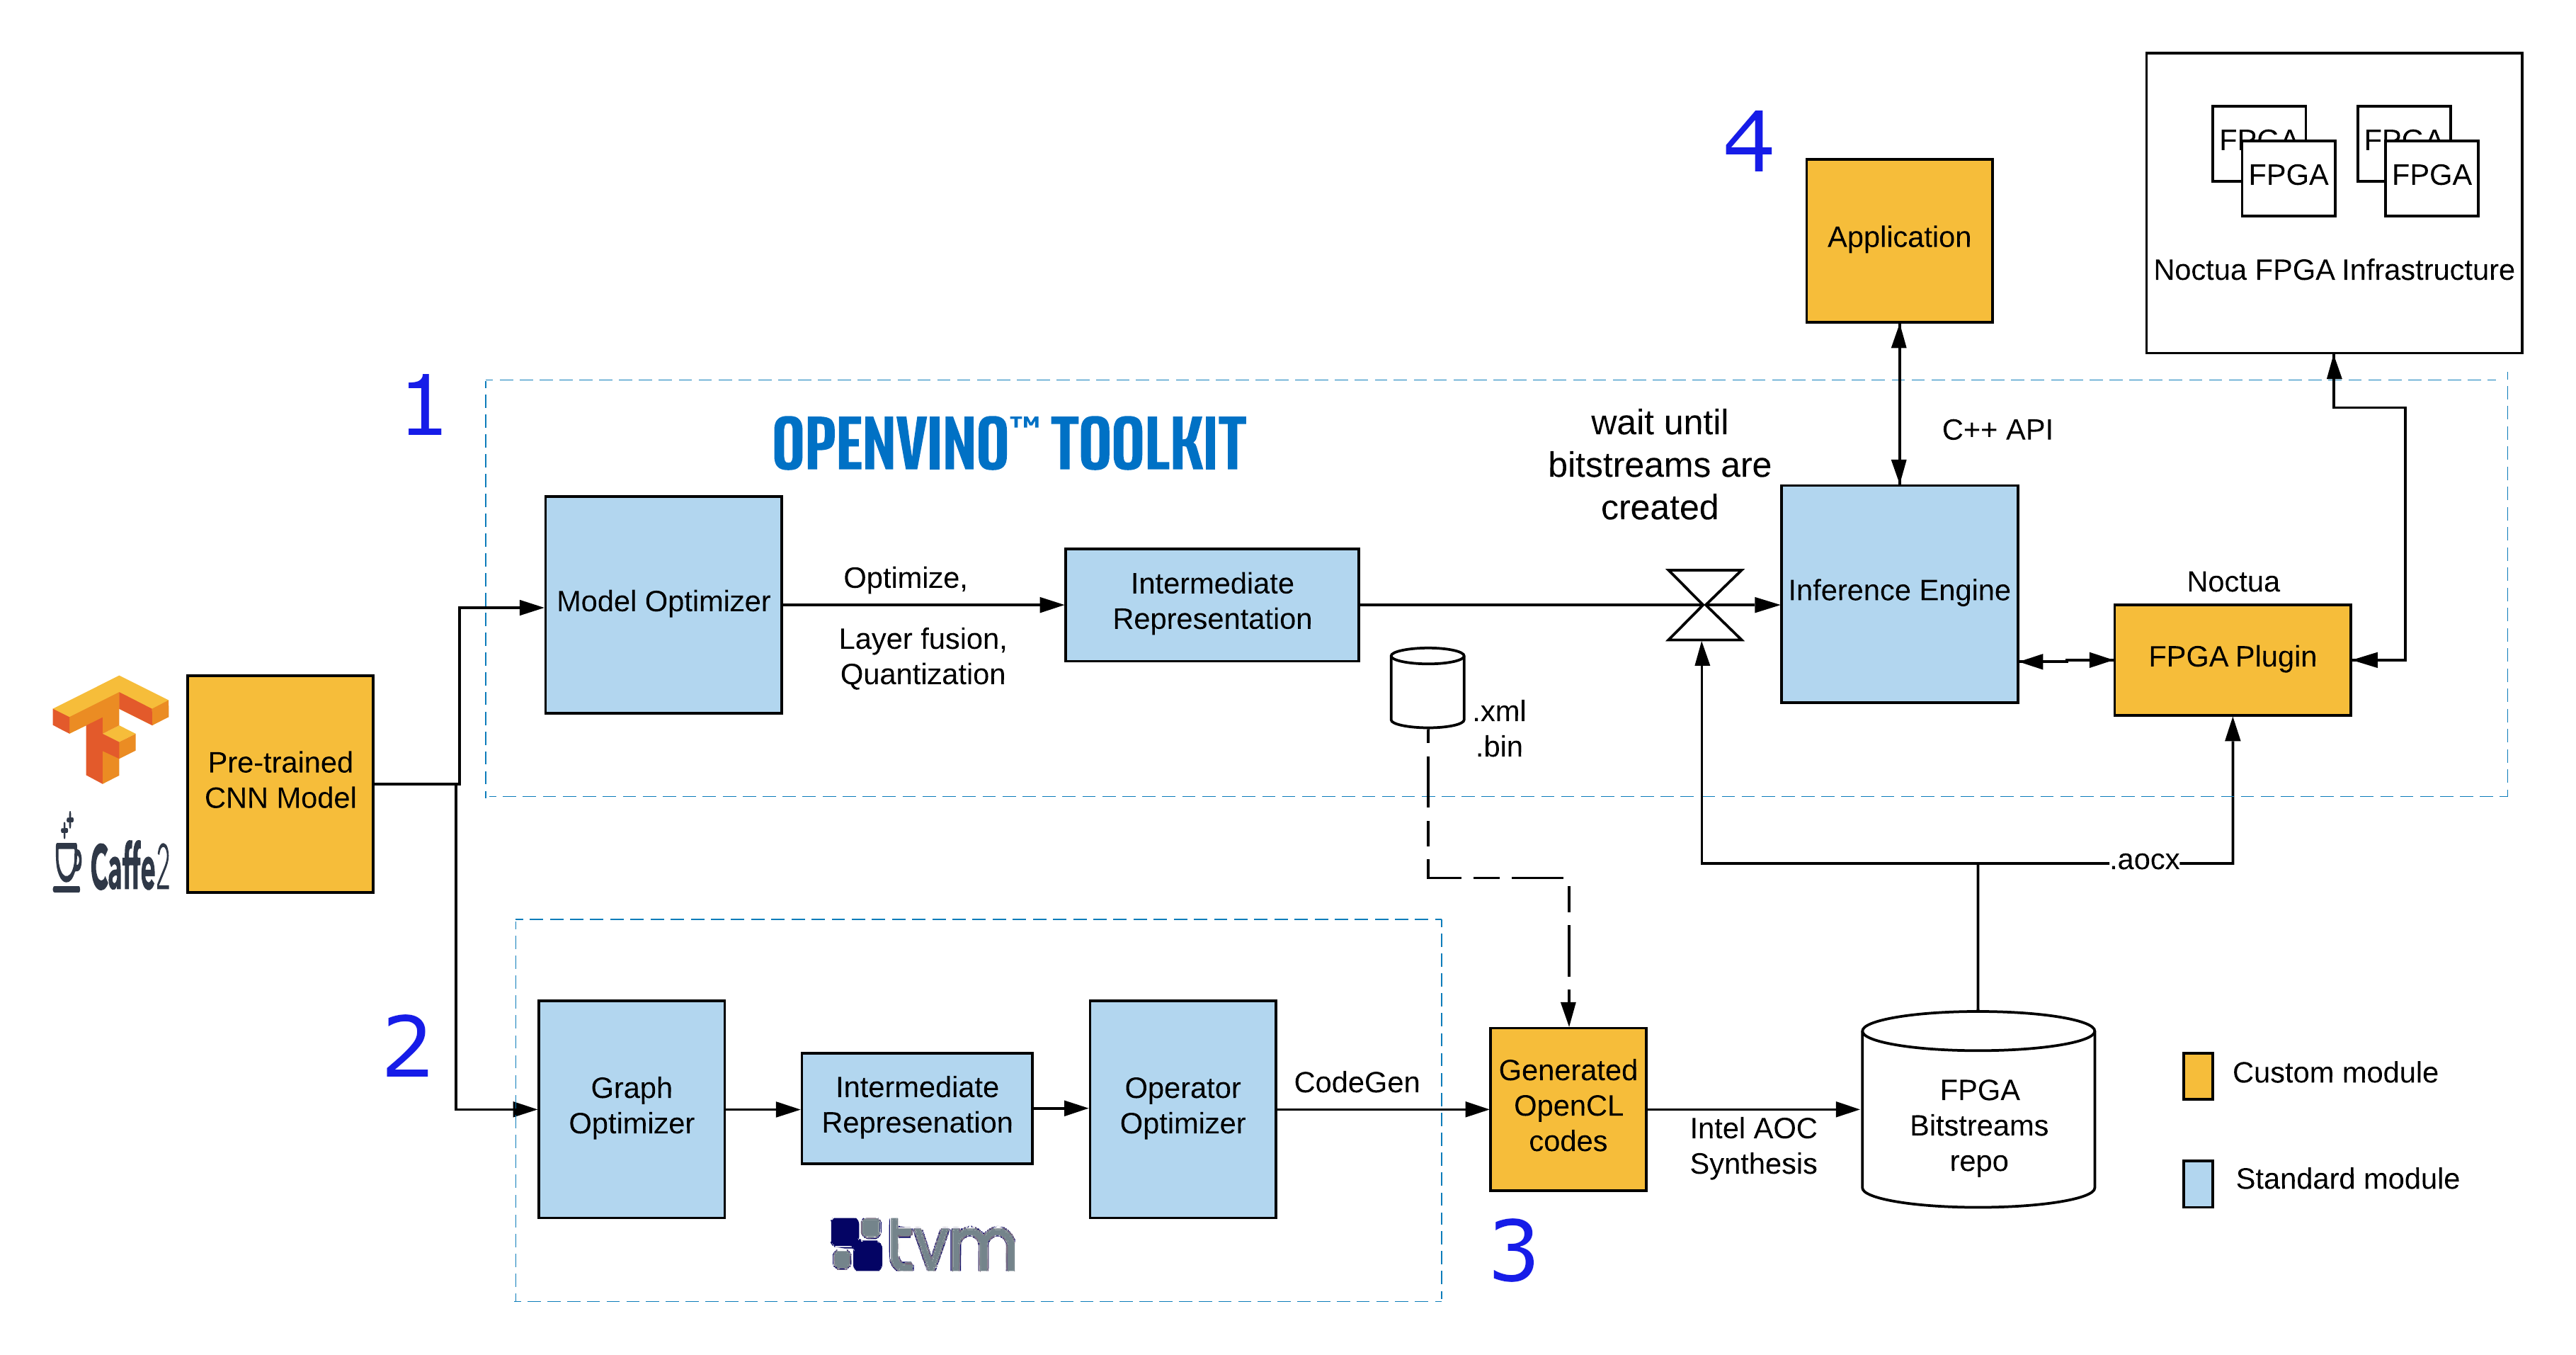
\includegraphics[scale=1,width=\textwidth]{img/CustoNN2_Workflow_New.png}
    \caption{CustoNN2 Project Workflow}
    \label{fig:custonn2_workflow}
\end{sidewaysfigure}
Figure \ref{fig:custonn2_workflow} describes the workflow of the project group. As mentioned in Chapter \ref{chp:Toolkits}, we used two toolkits in our project. The workflow has four following important steps(numbered in Figure \ref{fig:custonn2_workflow}):
\subsection*{Step 1: Generating OpenVINO IR}
First starting with OpenVINO, we feed the downloaded pre-trained CNN model to the OpenVINO Model Optimizer. In Model Optimizer, the trained model in the form of \textit{protobuf} file undergoes optimizations and and get converted to a file format which can be read,loaded and inferred by OpenVINO Inference Engine. The output of Model Optimizer is an Intermediate Representation (IR) consisting of an XML file and a binary(.bin) file. The XML file contains the description of the CNN model topology and the .bin file contains the biases and weights binary data. 
 
\subsection*{Step 2: Generating OpenCL Kernels}

We feed the downloaded pre-trained frozen CNN model to the NNVM compiler. The compiler frontend parses the model generating  NNVM expression (sym) and parameters (params) from the model. We set the optimization level and based on this level graph optimization techniques such as Operator Fusion and DataLayout Formatting are performed. The output is an Intermediate Representation (IR) which contains two files. The first is a JSON file that contains the optimized computational graph and the second file is a PARAM file that contains the quantized weight of the CNN model. This high-level IR and optimized computational graph are sent to lowering function with a TVMRegister API call which generates lower-level IR and graph. This code is then passed to the CodeGen module of the TVM toolkit and based on the target hradware it generates the required OpenCL kernel codes. The generated OpenCL kernel codes can be specific to a particular topology or it can be layer-specific which can be used in multiple topologies.

Step 1 and 2 are independent of each other and can be executed parallely.
 
These generated OpenCL kernel code needs to be customized to be compatible with OpenVINO FPGA plugin. After customization these kernel code are then synthesized for Stratix 10 FPGAs in the Noctua cluster and we create a repository of these bitstreams. We use TVM toolkit solely as a code generator for OpenCL kernel codes.

\subsection*{Step 3: Integrating toolkits and bitstream synthesis}
By default, the toolkits cannot work together and hence we need explicit integration in our workflow. The dotted arrow line in the Figure \ref{fig:custonn2_workflow} shows the integration point.
The OpenCL kernels generated by TVM are customized to be compatible with OpenVINO FPGA plugin. Here we manually change the OpenCL kernel names according to the OpenVINO IR layer names. Along with the layer names, for integration we had to change the layout of the some kernels (for ex: Concat kernels in GoogLeNet) from NHWC to NCHW. Once all the kernels are tested for correctness, we divide the OpenCL kernel file into multiple kernel files accordig to the scaling strategy. After customization these kernel code are then synthesized for Stratix 10 FPGAs in the Noctua cluster and we create a repository of these bitstreams. 
  
\subsection*{Step 4: Inference}
We have to wait till Step 3 is completed and all the bitstreams are synthesised without any errors.

The inference is done using a C++ application which uses OpenVINO Inference Engine and FPGA plugin  for the image classification in the Noctua cluster. The application is executed on multiple nodes of the Noctua FPGA nodes simultaneously according to the scaling strategy. The synchronisation between multiple application instances are done with the help of MPI barrier.

First, according to the scaling strategy the FPGA plugin will flash the appropriate bitstreams on the devices at each Noctua FPGA node. Once all the bitstreams are flashed on the FPGAs, the plugin will parse the Intermediate Representation (IR) information and start the inference on the FPGA by launching the OpenCL kernels.
After the execution of whole CNN topology, the instance of the application running on the last FPGA node will give the inference results with the TopN image classification with its Softmax values.



\begin{figure}[!htbp]
   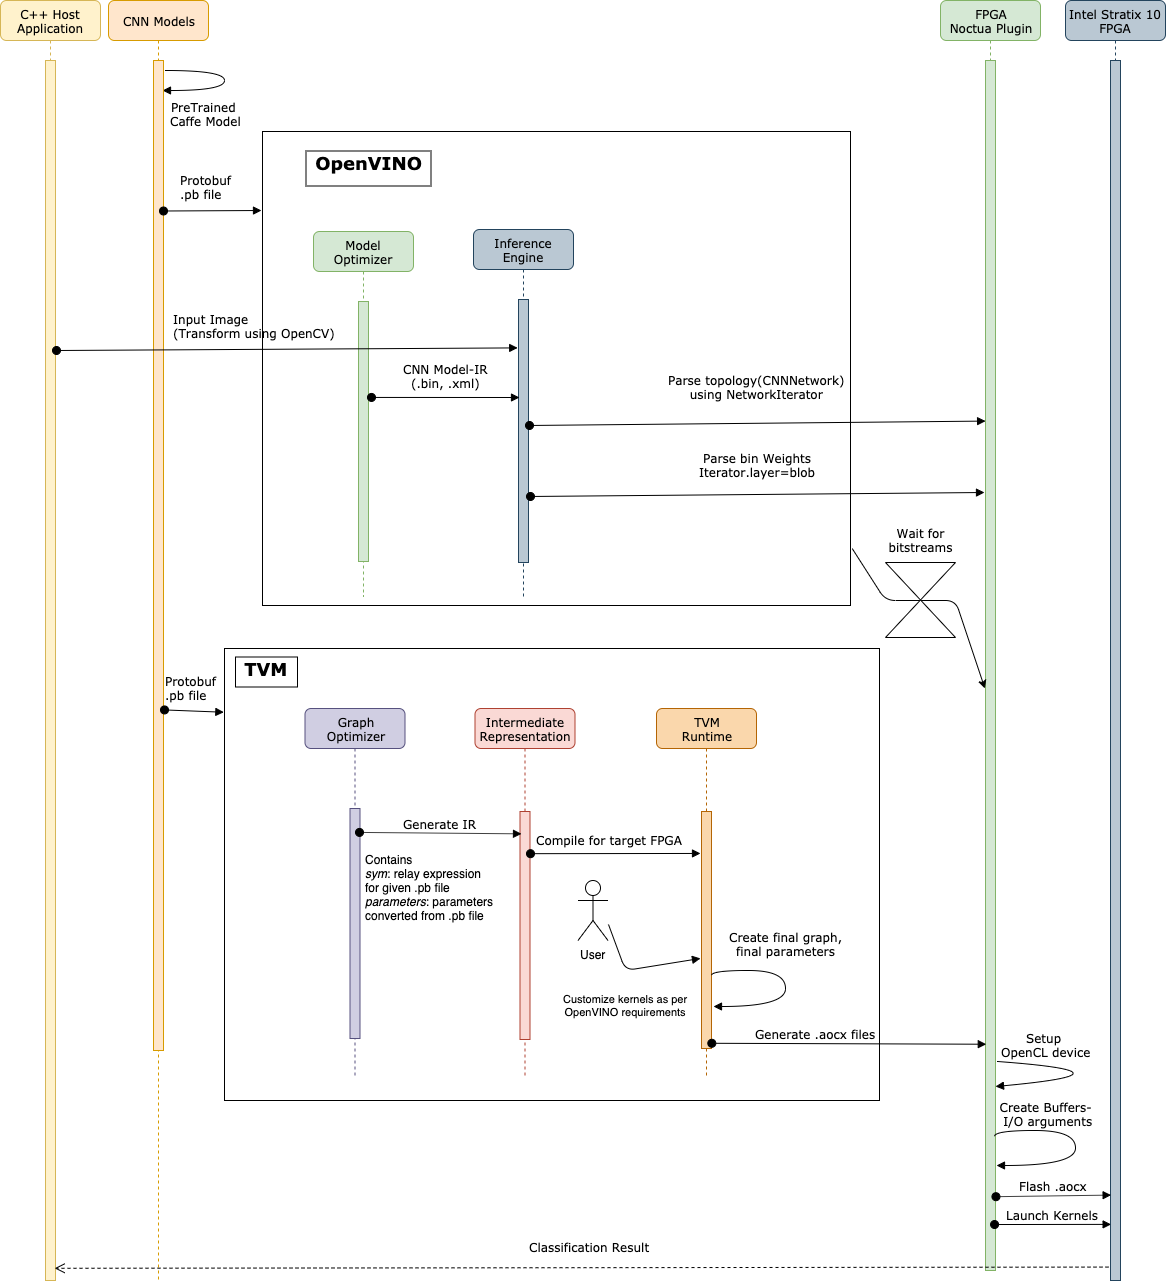
\includegraphics[width=\textwidth,height=\textheight]{img/udd.png}
   \caption{Sequence Diagram of the Project Workflow}
\end{figure}

\chapter{Designs and Performance Modeling}

Two CNN models - GoogLeNet (Inception V1) and Resnet-50 - were implemented on FPGAs in the project. The choices were made based on :  
\begin{itemize}
  \item complexity of CNN models
  \item relevance in the industry
  \item accuracy of the models
  \item availability of pre-trained weights and biases
  \item project timeline
\end{itemize}  
We wanted to implement CNN models complex enough to require scaling over multiple FPGAs. This requirement was a direct consequence of our initial objective of wanting to scale over multiple FPGA devices. Here, the complexity of the model refers the number of hidden layers present in the model. GoogLeNet - with  22 layers - and ResNet - with 50 layers- are deep enough to warrant using multiple devices for implementing them.

As the winners of Imagenet Large Scale Visual Recognition Challenge(ILSVR) 2014 and 2015 respectively, GoogLeNet and Reset are quite well known in the industry. With an inference accuracy nearing human capability - GoogLeNet or exceeding human capability -Resnet-152, these models are very popular in the machine learning community. We chose to implement a smaller version of Resnet called Resnet-50. Even though Resnet-50 is relatively shallow compared to Resnet-152, it still has a very high accuracy.

Since our objective was to implement an inference engine and not training an inference engine, it was imperative to work with models for which weights and biases were readily available. The popularity of GoogLeNet and ResNet in the machine learning community means that the weights and biases are available freely in the form of frozen models. "Frozen models" are special files where all the required parameters - weights,biases,graphs etc - of a model are saved.

We stopped at two models as the time required to implement more models was significant and would have forced us to spend less time on other important tasks. And the main objective of our project - implementing CNNs on FPGAs - was met when we successfully implemented GoogLeNet and ResNet. We felt no additional findings would come out of implementing another CNN model on FPGAs.

Implementation of such complex applications on FPGAs calls for "Performance Modeling". Performance Modeling entails the detailed study of how kernels get executed on FPGAs and allows a design engineer to understand the bottlenecks, performance limiting issues, general performance, etc. of kernels. Using performance modeling and making an educated assumption about the final design clock frequency, a design engineer can also predict the approximate run-time of a design.
For all the designs which we implemented, we also created models to explain the performance of our designs.    

In the next few sections, we explain in detail how we implemented different FPGA designs of GoogLeNet and ResNet-50 and the accompanying performance models.



\section{GoogLeNet}

The first CNN model we implemented was GoogLeNet. The idea of multiple designs of GoogLeNet was hatched to see the difference in performances when different levels of optimizations are applied at OpenCL level and architectural level. 
We were able to implement three major designs for GoogLeNet :
\begin{itemize}
  \item Baseline
  \item DSP Usage Optimized
  \item Hybrid Design
\end{itemize}  

\subsection{GoogLeNet Baseline}

GoogLeNet Baseline was implemented by modifying the OpenCL code generated by TVM for GoogLeNet. We modified the generated code to meet the requirements of our plugin. Some of the major modifications which were performed are :
\begin{itemize}
  \item renaming kernel names
  \item merging ReLUs with Convolutions
  \item rewriting Concatenation layers to support NCHW layout
  \item removing transpose kernels
\end{itemize}  
We had to rename kernels as the naming convention used by TVM and our plugin was not the same. We  had to make sure that we had all the kernels in OpenCL code that the plugin expected to launch.

By merging ReLUs with Convolutions, we optimized away the need to send data from one kernel(Convolutions) to another(ReLUs). This preoptimization step is used in the Deep Learning Community widely as ReLUs are basically light weight operations and do not warrant separate kernels.

By analysing our plugin, which is an extension to OpenVINO, and TVM, we realized that the layout used by OpenVINO and TVM were quite different. OpenVINO uses NCHW layout scheme whereas TVM uses NHWC layout scheme in Concatenation layer and NCHW layout scheme in all the other layers. To convert from NHWC to NCHW, TVM had generated transpose kernels. We modified all the Concatenation kernels to output NCHW thereby eliminating the need to have transpose layers.  

The modified code was first compiled to run on an FPGA emulator - Intel® FPGA Emulation Platform for OpenCL . We verified the functional correctness of the modified code by comparing the values output by our modified code with the values output by TensorFlow implementation of the same model.  

The initial reports generated for this modified OpenCL code indicated that this implementation of GoogLeNet needed a lot more resources than is available on a single Stratix 10 board. In order to successfully run this design on FPGAs, there was a need to divide the design into smaller parts. By dividing the design into ten smaller parts, we took advantage of the inherent logical divisions present in GoogLeNet topology. As  described in \ref{GoogLeNet_Topo}, every inception module is followed by a  Concatenation layer. Thus, we divided our design into ten smaller parts.  The first part is a purely feed forward design. The rest of the parts contain at least one inception module each and other layers as shown in Figure \ref{fig:GoogLeNet_division}


\begin{figure}[h!]
  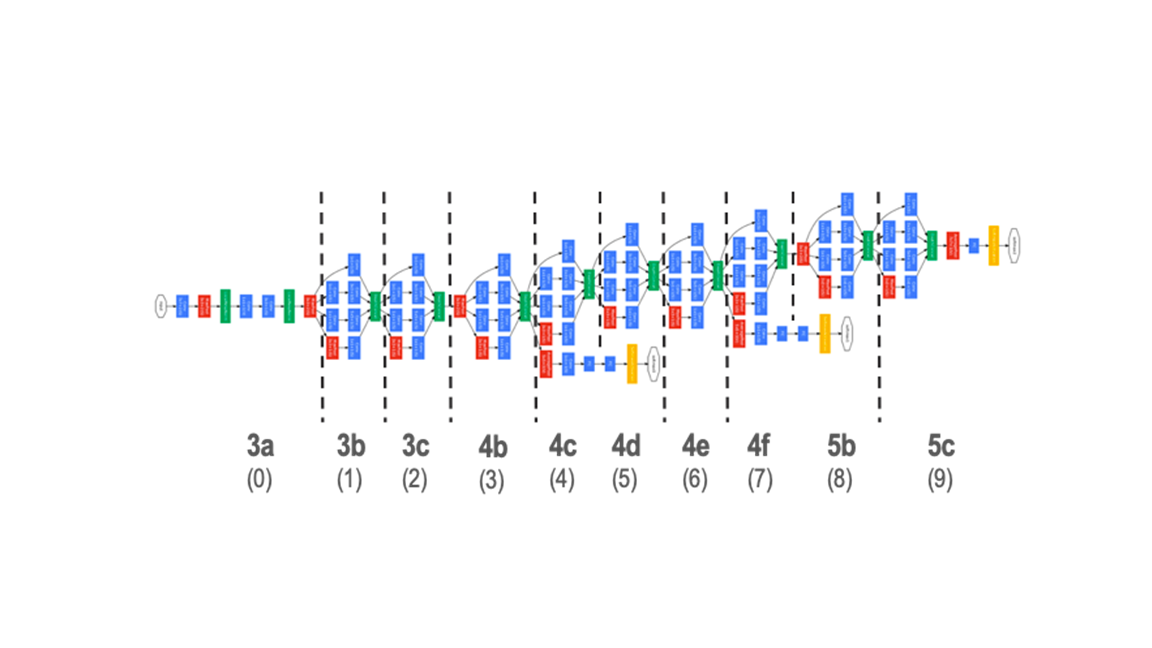
\includegraphics[width=\textwidth,height=\textheight,keepaspectratio]{img/GoogLeNet_division.png}
  \caption{Division of GoogLeNet topology}
  \label{fig:GoogLeNet_division}
\end{figure}
 
The ten resulting OpenCL bitstream files (in aocx format) were named as "inceptionX", where X represents the ordinal value(shown in brackets) of the part the file is made of as shown in Figure \ref{fig:GoogLeNet_division}. For example, the file containing the description of part 3a in Figure \ref{fig:GoogLeNet_division} was named as "inception0.aocx". This naming convention plays a crucial part in deciding the order in which the bitstreams are flashed on multiple devices as discussed further ahead in this section.  

We envisioned scaling over ten devices by using the scheme shown in Figure \ref{fig:GoogLeNet_Scaling}

\begin{figure}[h!]
  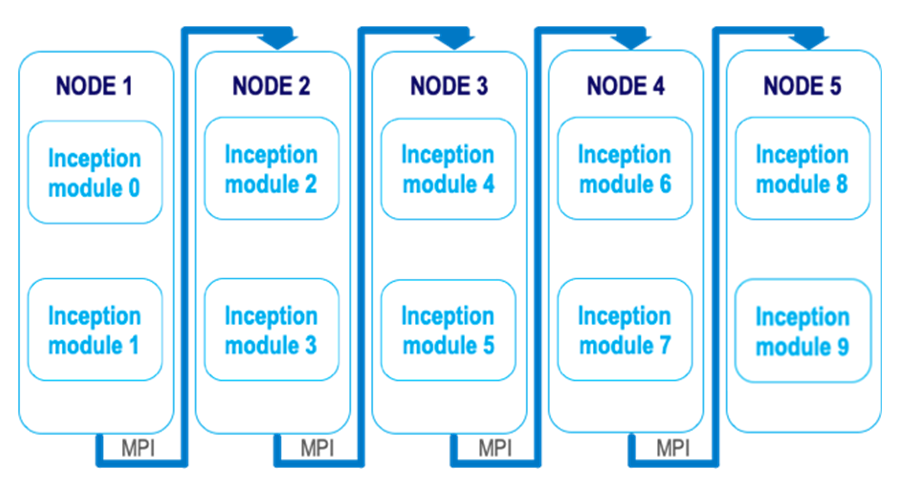
\includegraphics[width=\textwidth,height=\textheight,keepaspectratio]{img/GoogLeNet_Scaling.png}
  \caption{Scaling of GoogLeNet topology over 10 FPGAs}
  \label{fig:GoogLeNet_Scaling}
\end{figure}

Each Noctua FPGA node has two FPGAs. Thus, this scheme requires five nodes to execute ten parts of GoogLeNet. Initially, we had two main challenges - flashing the right bitstreams on to the right devices, and transferring data from one node to another.

The first challenge - flashing the right bitstreams on to the right devices was solved using Message Passing Interface (MPI). This is shown in Code \ref{code:MPICode_plugin}.  


\begin{code}[!htb]
 \begin{minted}{c++}
 /* Snippet of test plugin - main.cpp */
        #include "mpi.h"
        MPI_Init(NULL,NULL);
        int rank;
        MPI_Comm_rank(MPI_COMM_WORLD,&rank);
        fpga_launcher(network,inputModel,imageNames,cnn_model,rank);
    
\end{minted}
\caption{testplugin/main.cpp}
\label{code:MPICode_plugin}
\end{code}

We included the MPI library and initialized it. We retreived the rank of the nodes and then passed the ranks as parameter to the function \texttt{"fpga\_launcher()"}. This function is present in \texttt{"noctua\_plugin /fpga\_plugin.cpp"}. With the ranks as parameters , this function handles the flashing of the bitstreams by calculating the parity of the ranks. These ranks in themselves are enough to identify the nodes(since the ranks are retrieved from the nodes). This is shown in Code \ref{code:MPICode_fpga_plugin}.

\begin{code}[!htb]
 \begin{minted}{c++}
 /* Snippet of noctua_plugin - fpga_plugin.cpp */
        #include "mpi.h"  
        
        std::string file1 = GoogLeNet_DIR+"inception"+std::to_string(2*rank)+".aocx" 
        std::string file2 = GoogLeNet_DIR+"inception"+std::to_string(2*rank+1)+".aocx"  
        
        std::string file1_xml = GoogLeNet_DIR+"inception"+std::to_string(2*rank)+".xml"
        std::string file2_xml = GoogLeNet_DIR+"inception"+std::to_string(2*rank+1)+".xml"   
        
        char f1_xml[file1_xml.length()];
        strcpy(f1_xml,file1_xml.c_str());  
        
        std::vector<std::string> first_kernels = xml_parser1(f1_xml);

\end{minted}
\caption{noctua\_plugin/fpga\_plugin.cpp}
\label{code:MPICode_fpga_plugin}
\end{code}

The naming convention we used for the bitstreams allowed us to pick the appropriate bitstreams by  name and thus, we successfully flashed the bitstreams on to the correct devices. We also read and parsed the XML files which were generated along with the bitstreams. These XML files contain information about the kernels present in a particular bitstream. Using this information, we launched all the valid kernels as needed. 

The second challenge - transferring data from one node to another was also solved using MPI. The devices in a node share the same memory address space and thus, they had access to each other`s global memory.   

The data transfers from one device to another device in the same node were handled using global memory. The data transfers from a device on one node to a deivce on another node was handled using two MPI functions : MPI\_Send() and MPI\_Recv(). We called MPI\_Send() at the last kernel of every node except for the very last one. And the first kernel of every node except for the first one had a function call for MPI\_Recv(). The visual representation of this scheme is show in Figure \ref{fig:GoogLeNet_Scaling}. Thus, using  MPI\_Send() and MPI\_Recv(), we were able to transfer data from one node to another, allowing us to truly scale over multiple devices.

This implementation of GoogLeNet is completely devoid of optimizations barring a few implementation related optimizations (merging ReLUs with Convolutions etc). Thus, it was named as "Baseline". When we executed this baseline version of GoogLeNet over ten devices, the design took 67.47 seconds to classify one image.  

By any measure, this execution time is extremely slow when it comes to designs running on accelerators. To see why this baseline was slow , we had to first do performance modelling to explain this run time.

The performance modeling for designs like this involves determining
  Multiply-Accumulate (MAC) operations in design , amount of global memory transfers, run-time, clock frequency ,and the initiation intervals (IIs) and latency of loops.

The run-time and clock frequency are ascertained from "profile.mon" files.   
The profiling data generated by Intel SDK for OpenCL Applications are stored in files named "profile.mon". These are generated whenever kernels are executed on FPGAs. During synthesis, it is necessary to enable -profile flag if one wishes to have profiling data generated for their designs (when they are executed on FPGAs). We had enabled this flag for all our designs and thus had access to profiling data for all our kernels.

The first two steps of performance modeling for baseline - determining number of operations and amount of global memory transfers - were done using a script developed by the team. The script was written in Python and made use of ANTLR4 lexer and parser generator tool. OpenCL follows the grammar of C language. Keeping this in mind, we generated a parse tree of all the ten OpenCL source files with the help of ANTLR4 using C.g4 grammar file (Grammar files use the "g4" file extension). We wrote a script to walk the parse tree to determine the number of MAC operations and the amount of global memory transfers present in a file.

The next two steps of performance modeling - determining execution time and clock frequency - were done by opening profile.mon files using the profie.mon viewer provided by Intel SDK for OpenCL. The profiling data records execution time of each and every single kernel which get executed to completion. And the overall frequency at which the kernels in a given OpenCL file run is also recorded in these files.The initiation intervals and latency of different parts of loops is gathered from HTML reports. Taking all this into consideration , the performance modeling of baseline design revealed the details tabulated in Table \ref{tab:GoogLeNetBaselinePerfModel}.
\begin{table}[!htb]  
 \centering
 \captionsetup{
 justification = centering
}
\caption{GoogLeNet Baseline Performance Model}

    \begin{tabular}{|c|c|}
    \multicolumn{2}{c}{\textbf{}} \\ \hline

     Number of Operations    &   2.9 Billion \\ \hline
      Global Memory transfers &   20.9 GB            \\ \hline          
      Execution time    &  67470 ms    \\ \hline
      Operations/second   &   0.04 GOPS \\ \hline
      Operations/cycle &   0.216             \\ \hline
      Operations/byte       &   0.143     \\ \hline
      Global Memory/second & 311 MBps  \\ \hline

    \end{tabular}
    
    \label{tab:GoogLeNetBaselinePerfModel}                            

\end{table}  

Throughput, as defined in Chapter \ref{chp:Metrics}, for this design is 0.014 images classified per second. Since  the Top-5 accuracy of the model is the same as the one given in the literature (89.9\%), the only factor that could change when calculating Rate Correct Score is the latency. And for this case , Rate Correct Score is calculated as the ratio between accuracy from literature and the latency of our implementation of GoogLeNet. This comes to be  1.33 per second.

The HTML reports revealed that the initiation intervals of most of the loops were much bigger than 1. And some of the loops were not pipelined because of loop-carried dependencies. We also observed from initial reports that the DSP usage of Baseline was quite abysmal. Baseline design was using less than 1\% of the total DSPs available on Stratix 10 board. This is shown in Figure \ref{fig:Report_Baseline}   


\begin{figure}[!htb]
  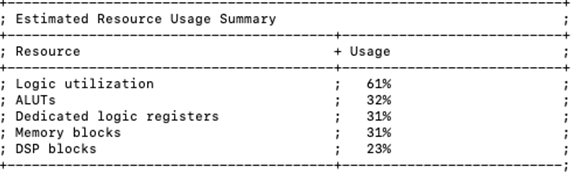
\includegraphics[width=\textwidth,height=\textheight,keepaspectratio]{img/Report_Baseline.png}
  \caption{Initial report of one of the files of Baseline Design}
  \label{fig:Report_Baseline}
\end{figure}

Though the estimated DSP blocks usage is 23\% in Figure \ref{fig:Report_Baseline} , in reality less than 1\% of the DSP blocks is used by the design. 

Furthermore, the profiling data for baseline also indicated that the occupancy of  parts of the code where the MAC operations take place were extremely low - in the neighbourhood of 0.1\%. 

Since none of the loops were unrolled, and because of loop carried dependencies (compiler would not unroll automatically), we could estimate that only two operations would take place in one cycle (the inner most loop has two operations - one multiply and one addition). If the loops were unrolled , then the design could have utilized more number of DSP blocks in a single clock cycle thereby executing more number of operations per cycle. In reality (from measurements), we saw that the real operations/cycle was 0.216 (as opposed to an estimated 2 ops/cycle). This indicated that even the resources (DSP blocks specifically) which were assigned were underused. The memory transfers from global memory too was very slow. Additionally, the low utilization of DSP blocks indicates the biggest problem with this design - lack of parallel execution of operations.  

As shown in Figure \ref{fig:GoogLeNetBaseline_Runtime_Graph} , we notice that the slowest kernel was at the top of the design - a 3x3 convolution kernel. It took about 18s to get executed. "Inception0" has the most number of operations in the design and it is not surprising that it took the major part of the total time to get executed to completion. Every other 3x3 convolution kernel also took significant amounts of time to get executed. Other kernels - like padding and concatenation kernels were relatively fast. The graph in Figure \ref{fig:GoogLeNetBaseline_Runtime_Graph} helps us visualize the execution sequence of the design. Once execution on the first FPGA is over, the execution takes place in the second one. And once the image is processed in the second FPGA, it moves on to the third FPGA and so on. Most of the times the FPGAs remain idle as can be seen from the empty regions in the time axis in the graph. The total execution time, as mentioned above, was 67.47 seconds.

The rest of the kernels - consisting of Maxpools, Concats, Padding etc, are shown in gray in Figure \ref{fig:GoogLeNetBaseline_Runtime_Graph}. They take up minimal amount of time to get executed in this design.

\begin{figure}[!htb]
  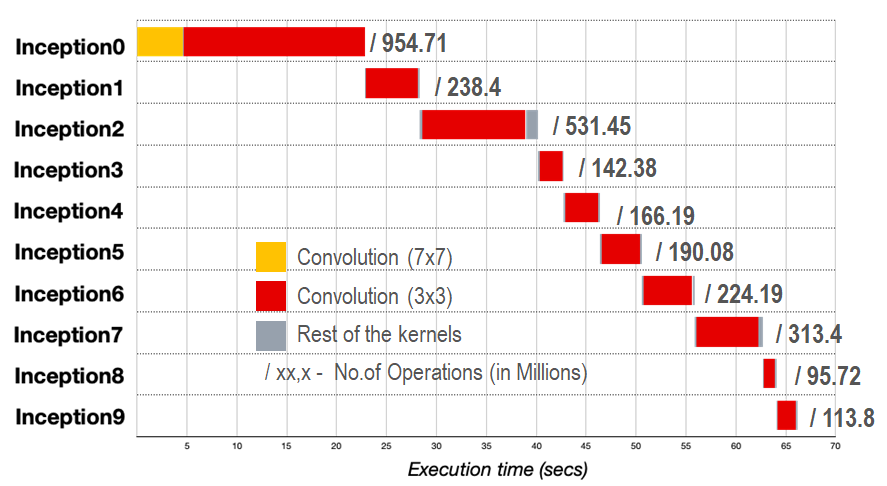
\includegraphics[width=\textwidth,height=\textheight,keepaspectratio]{img/GoogLeNetBaseline_Runtime_Graph.png}
  \caption{Execution time - GoogLeNet Baseline Design}
  \label{fig:GoogLeNetBaseline_Runtime_Graph}
\end{figure}


In conclusion, the reasons for baseline version of GoogLeNet performing so badly are :
\begin{itemize}
    \item low DSP blocks usage
    \item initiation intervals greater than 1
    \item loop carried dependencies 
    \item global memory transfers
    \item FPGAs remain idle most of the time
\end{itemize}

To speed this design up, we decided to solve the problem of low DSP usage. This leads us to our next section - GoogLeNet DSP Usage Optimized.

\subsection{GoogLeNet DSP Usage Optimized}
The biggest problem with the baseline implementation of GoogLeNet, according to us, was the very low utilization of DSP blocks (or just DSPs). With an estimated two operations per one clock cycle, it is easy to see that such a design is doomed to have very bad performance (given the clock frequencies are in hundreds of MHz range).
 
Keeping this in mind, we decided to increase the number of operations our design could perform in one clock cycle. As was noted in the previous section, an increase in number of DSPs could result in more number of operations getting executed in one clock cycle. If the inner most loops are unrolled, then the compiler allocates an increased number of resources to carry out all these unrolled operations in parallel (given that these operations have an II of 1 - no dependencies between operations). 
 
 Thus, in order to have an increased allocation of DSPs to our design, we made use of interrelated  optimization techniques like : 
 \begin{itemize}
     \item Loop Unrolling
     \item Loop Pipelining
     \item Using Shift Registers
     \item Using Local Memory
\end{itemize}

When these optimization techniques were applied on the baseline design, we were able to increase the total DSPs by a margin of just 1\%. The problem lay in the fact that we were limited by the amount of unrolls we could perform. After unrolling by a few factors, we noticed that the other resources` usage would go beyond what was available on Stratix 10 boards.

This problem was intrinsic to the convolution logic the design had. We observed that the operations were happening depth wise first and then along the spatial dimension. This convolution logic is depicted in Figure \ref{fig:GoogLeNet_Conv_logic}.This logic works by first operating on pixels along the red arrow first (depth wise). Then it moves to the next pixel in the spatial dimension and continues working with the pixels depth wise. More concretely, the problem with this approach is that it calculates the first pixel of each slice of image. If the image is of dimensions 256x256, the array values with index 0, 256x256, 256x256x2, and so on will need to be calculated. To access each of these pixels makes the design slow because the location of these pixels are not close to each other. And even with a slightly small unroll factor, one needs to duplicate the whole image array.

\begin{figure}[!htb]
  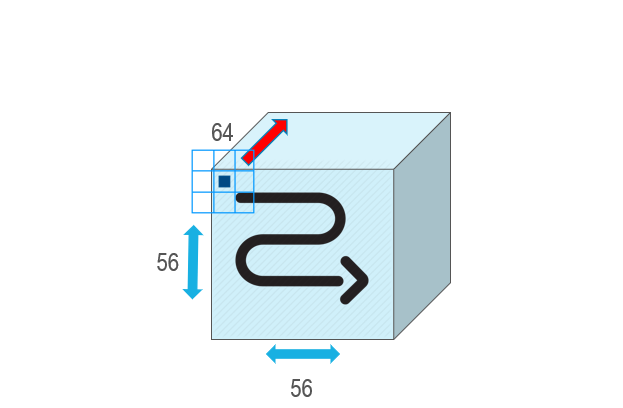
\includegraphics[width=\textwidth,height=\textheight,keepaspectratio]{img/GoogLeNet_Conv_logic.png}
  \caption{Example of Convolution Logic}
  \label{fig:GoogLeNet_Conv_logic}
\end{figure}

Unrolling the loops which work with the above logic results in replicating the big image-data (as shown in Figure \ref{fig:GoogLeNet_Conv_logic}, dimensions vary from kernel to kernel) multiple times. After just a few unrolls, we start to reach the limits of resources available Stratix 10 board. Thus, the idea of simply unrolling the inner most loop just would not work with the logic present in this design,

To overcome this problem, we decided to change the order of the loops such that the calculations happen on the spatial plane first. Once the convolutions happen on spatial "slice" of image-data, the operations are performed on the next slice of image-data. From Figure \ref{fig:GoogLeNet_Conv_logic}, this logic would appear as operations happening along the black arrow first , and then once the pixels in the spatial plane are done being operated, the operations are repeated on the next spatial plane, one channel deeper. This continues until all the pixels are operated upon.  

With this new logic, when the inner most loop is unrolled, only a slice of image-data needs to get replicated. When we applied this logic to all the kernels of GoogLeNet, we saw a remarkable improvement in the usage of DSP blocks. The reports generated after modifying the logic of convolutions indicated that the estimated resource usage of DSP blocks increased by a margin of 47\% for most of the files. This was achieved keeping all the other resources well within the limits imposed by the board. 

Unfortunately, the synthesis of these modified files did not succeed. The compiler/synthesis tool threw errors regarding placement and routing. It looked as if the synthesis tool just could not fit any of the designs with a high usage of DSP blocks.   
One of the solutions proposed to solve this problem was reducing the unroll factors in our kernels so as to decrease the need for a high number of DSP blocks. This process entailed reducing the unroll factors, keeping the designs for synthesis on Noctua Compute nodes, waiting for anywhere between 6 hours to 24 hours for the synthesis tool to inform us whether the synthesis succeed or not . We had to reduce the usage of resource(specifically DSP blocks) severely times to finally get designs  which would get synthesized. In other words, we used trial and error method on all the ten files to eventually get bitstreams for our designs,  

The resulting designs made use of more DSP blocks than the baseline version of GoogLeNet, but less than what we could have achieved if the synthesis tool had succeeded in synthesizing the designs in which we had heavily unrolled the inner most loops. Nevertheless, we decided to call this design - GoogLeNet DSP Usage Optimized.This design of GoogLeNet, on average across all the ten files, made use of about 10\% of DSP blocks available in the boards.

From the tutorials, the team had learnt that just increasing DPS block usage in itself is not enough to extract better performance from a design. We made sure that all the initiation intervals of the loops were 1 or just about 1. And we also ensured that all the loops were pipelined. The latencies of the loops were not given much thought because the pipelined nature of the loops and the extremely large number of clock cycles to execute the designs dwarf over the values of latencies present in our design.   

To achieve all of the improvements to our design mentioned above, we had to introduce temporary variables and  also do extra operations. This can be seen from Figure \ref{fig:GoogLeNetDSPOpt_Runtime_Graph}. When compared to Figure \ref{fig:GoogLeNetBaseline_Runtime_Graph} , we see that the operations in each inception block has gone up. For example, in baseline design , there were 954.71 Million operations present in "inception0". But in case of DSP usage optimized design, there are 1200 Million operations in "inception0". 

\begin{figure}[!htb]
  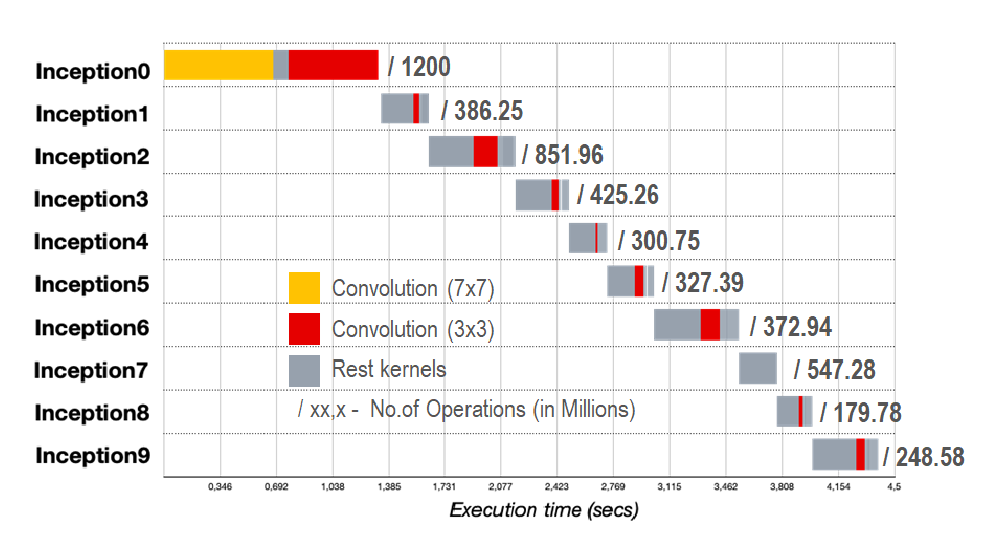
\includegraphics[width=\textwidth,height=\textheight,keepaspectratio]{img/GoogLeNetDSPOpt_Runtime_Graph.png}
  \caption{Execution time - GoogLeNet DSP Usage Optimized Design}
  \label{fig:GoogLeNetDSPOpt_Runtime_Graph}
\end{figure}


When the DSP usage optimized design was executed on all the 10 FPGAs, the design got executed in 4.41 seconds ! This was a noteworthy improvement in performance compared to the baseline design. 

The performance modeling for this design was not performed using the Antlr4 based tool. We were not able to extend the tool to account for the numerous changes that is present between the baseline design and the DSP usage optimized design.


\begin{table}[!htb]                          
 \centering
 \captionsetup{
 justification = centering
}
 \caption{GoogLeNet DSP Usage Optimized Performance Model}
    \begin{tabular}{|c|c|}
    \multicolumn{2}{c}{\textbf{}} \\ \hline

     Number of Operations    &   4.8 Billion \\ \hline
      Global Memory transfers &   2.09 GB            \\ \hline          
      Execution time    &  4814 ms    \\ \hline
      Operations/second   &   1.01 GOPS \\ \hline
      Operations/cycle &   6.5             \\ \hline
      Operations/byte       &   2.43 \\ \hline
      Global Memory/second & 0.43 GBps  \\ \hline

    \end{tabular}
    
    \label{tab:GoogLeNetDSPPerfModel}                            

\end{table} 

The performance modeling for the DSP usage optimized design is tabulated in Table \ref{tab:GoogLeNetDSPPerfModel}. Throughput, as defined in Chapter \ref{chp:Metrics}, for this design is 0.23 images classified per second. Since accuracy of the model is same as the one given in the literature (89.9\%), the only factor that could change when calculating Rate Correct Score is the latency. Similar to GoogLeNet baseline design, Rate Correct Score is calculated as the ratio between accuracy from literature and the latency of our implementation of GoogLeNet. For this design it is 20.38 per second. 

We noticed two major problems from profiling data - stalling problem and memory dependency. In convolution kernels, the part where we were reading slices of data from global memory had stalls reaching 50\%. Since the  the part where the computations were taking place were directly dependent on these slices of data, the computations themselves had a disappointing occupancy of just 6.0\%. 

At this stage, we had the choice of thinking of ways to improve the design by sticking to the ongoing design paradigm or to think of a new approach. To show that further improvements could be done on the current design, we proceeded to implement extra optimizations on one single file. We picked a file (in this case inception9 file), completely unrolled the section of the code where slices of image-data were read, completely unrolled the section of the code where computations took place. When we synthesized this design and ran the resulting bitstream on the FPGAs (in conjunction with the previously used bitstreams), we saw a remarkable improvement in the run time of the convolution kernel on which we had applied the extra optimizations. Previously, this convolution kernel had taken about 79.06ms to get executed. But with the extra unrollings, this convolution kernel got executed in 1.75ms! The profiling data for this kernel execution showed that the resulting stall for the part of the code where slice of image-data was read was just 0.91\% and the part of the code where the computations were happening had an occupancy of 96.3\%.  

This proved that with some simple unrolls to the loops responsible for reading the slices of image-data and to the loops where computations were being done, we could achieve significant amounts of performance gain. As they say, there are no free lunches in the world of FPGA accelerators. All these unrolling demands resources and we were already running out of resources.


Even though the run time for DSP usage optimized design is about 15 times faster than the baseline version of GoogLeNet, there is a lot of room for improvement. Because of the problems related to synthesis of heavily unrolled designs discussed in the beginning of this subsection , we could not bank upon further unrolling of inner loops to gain performance improvements. Thus, we had to look elsewhere to improve the performance of our design.


This search for a better way to run GoogLeNet on multiple FPGAs resulted in our next design - GoogLeNet Hybrid Design.

\subsection{GoogLeNet Hybrid Design}
Designs which rely on global memory for data transfers tend to be slower than designs which make use of channels to transfer data from one kernel to another. This can be ascribed to the fact that global memory data transfers are slower than data transfers made using channels.  

Designs which are completely based on global memory data transfers need the host to take care of data transfers. When the amount of data to be transferred is large, this ends up being a significant overhead. Another problem with designs based on global memory is that the kernels have to be launched sequentially. Otherwise, the kernels end up working on garbage data. The host code is responsible for launching the kernels at the right time and to control the access to global memory. Because of sequential launching of kernels, a designer cannot exploit concurrent sections of a design in a straightforward manner. 

Considering the above points, we decided to implement GoogLeNet using channels. There are two types of channels available in Intel FPGA SDK for OpenCL - internal and external.

Internal channels are used to transfer data between kernels present in the same device. External channels, in our case, are direct point-to-point connections between two devices that are abstracted in the OpenCL environment as Serial Channels. There are four such IO channels per device. In terms of networking terminology these can be called : north, east, west and south channels. External channels make it possible to send data from kernels present in one device to kernels present in another device. 

To implement a channel-based design, we replaced all the data transfers within a kernel file with internal channels. We used blocking channels in our design. The inclusion of channels made it necessary to change the plug-in code (host code) to handle the launching sequence of the kernels. The plug-in was modified to launch all the kernels on separate command queues. This change allowed us to launch all the kernels in a kernel file simultaneously. 


\begin{figure}[!htb]
  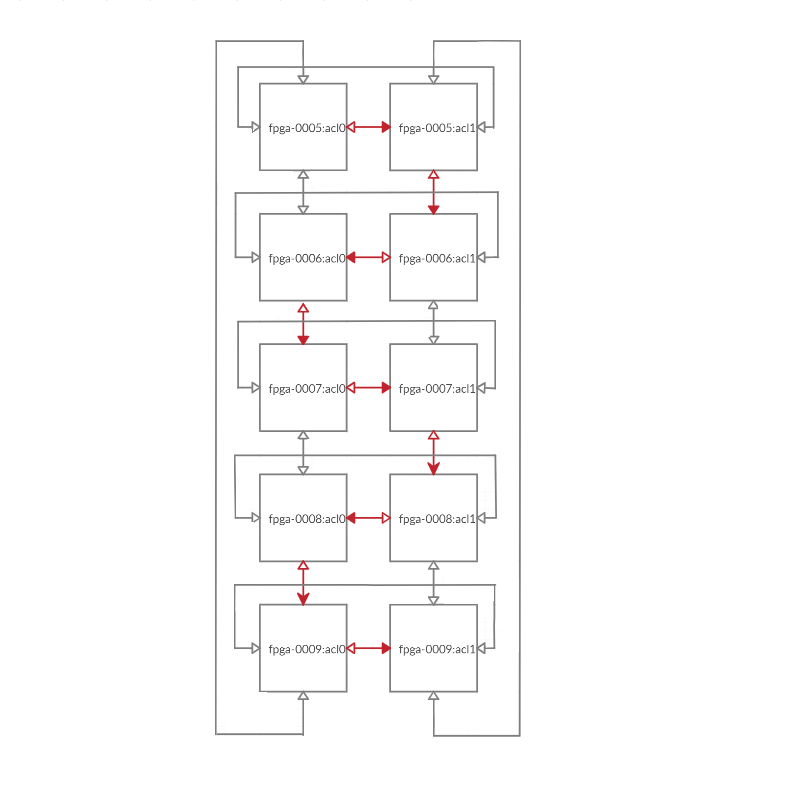
\includegraphics{img/Torus_Topology.PNG}
  \caption{Torus Topology}
  \label{fig:Torus_Topology}
\end{figure}

When it came to external channels, we had to choose between two designs : static design or dynamic design. With static design, the last kernel in a device is coded to output to a specific output channel and  the first kernel of a device is coded to read from a specific IO channel. This design would work great if the underlying hardware connections between different devices remain constant. If the point-to-point connections between two devices change for some reason, then one would have to rewrite the kernels to account for the change in topology, test them on emulators, put them for synthesis (which could take anywhere between 6 to 24 hours) and then try to run the new design on the new topology.




With dynamic design, instead of the first(last) kernel of a file reading(writing) from(to) one specific input(output) channel, the kernels could selectively read(write)  from(to) any one of the four IO channels available. By passing a "routing" argument and using if-else conditions in the first and last kernels of a file, it is possible to control the IO channels which feed-in or feed-out of a device. With dynamic design, it is possible to take routing decisions in the host code. Dynamic design helps in decoupling kernels from the underlying node topology.



If the routing decision is made in the host code, the routing decisions are made at compile time. This means that every time the node topology changes, one would have to change the routing parameters in the plug-in file, compile the plug-in and then run the design. We wanted to have routing decisions made at run-time to avoid this extra step of compilation. To this end, we outsourced the routing decision to a configuration file. We made use of an XML file where the node topology was described. This XML file was parsed during run-time to control the read/write operations on different IO channels. 

\begin{code}[!htb]
 \begin{minted}{XML}
<googlenet>
	<inception>
		<module>3a</module>           
		<input>0</input>				
		<output>3</output>
	</inception>
	<inception>
		<module>3b</module>
		<input>2</input>				
		<output>1</output>
	</inception>
...
...
...
	<inception>
		<module>5c</module>
		<input>2</input>				
		<output>0</output>
	</inception>
</googlenet>


\end{minted}
\caption{Snippet of topology.xml}
\label{code:topologyxml}
\end{code}
Thus, dynamic design allowed us to write kernels which were independent of the underlying node topology. Since we had ten different files which were to run on ten different devices, we had to look for topology with ten devices. Such a topology was set up for us by the admin of Noctua Cluster. The resulting topology is shown in Figure \ref{fig:Torus_Topology}. The XML used for setting up the required connection is shown in Listing \ref{code:topologyxml}. The XML contains information about the CNN topology and the input channel and output channel for every inception file. The directions of the IO channels are enumerated as : 0- North, 1- South , 2- West, 3- East. For example, module 3b, which corresponds to inception1.aocx , needs the input to be read from channel 2 i.e. from channel arriving from the West and it needs to write data into channel 1 i.e. to the channel going to South.  
The filled red arrows in Figure \ref{fig:Torus_Topology} depict the routing paths we chose to scale over multiple devices. The grayed out connections were not used. We passed this XML file as an argument to our plug-in and parsed the information in the XML to get the final routing data. 

The introduction of internal and external channels in our design can be visualized from Figure \ref{fig:GoogLeNet_Channels}. The yellow arrows depict the external (IO) channels. The blue lines indicate the internal channels. Every inception module has 4 branches - branch0, branch1 , branch2 and branch3 - shown in Figure \ref{fig:GoogLeNet_Channels} as the branches going from left to right. The kernels in these branches can be launched concurrently with respect to kernels in other branches.  This was not possible in the earlier designs as we were using only one command queue to launch our kernels.

\begin{figure}[!htb]
  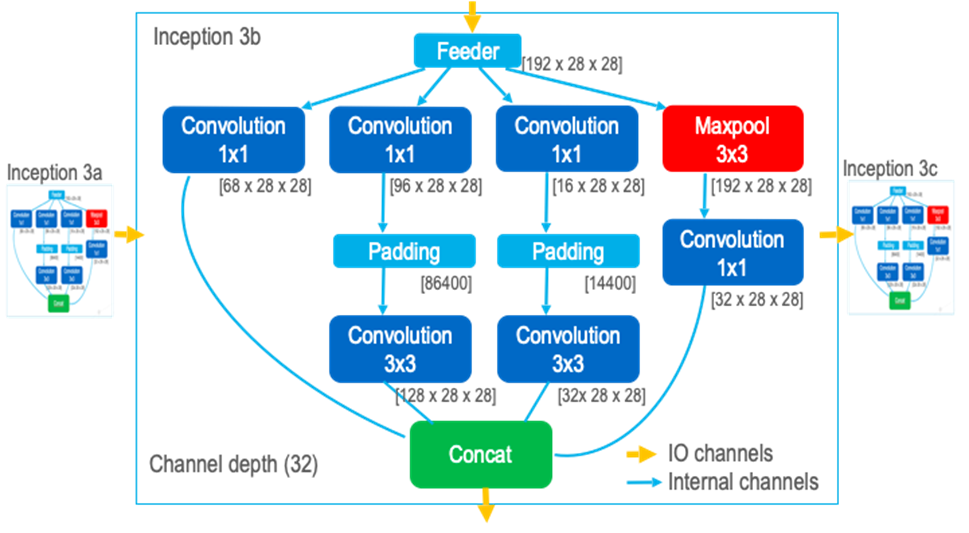
\includegraphics[width=\textwidth,height=\textheight,keepaspectratio]{img/GoogLeNet_Channels.png}
  \caption{GoogLeNet with Channels}
  \label{fig:GoogLeNet_Channels}
\end{figure}


Once all the files were converted to comply with channel-based design paradigm, we made the necessary modifications to the plug-in code. Before going for synthesis of the files, we made sure to test all the files on emulator. When the emulation was successful, we went ahead with synthesizing all the files into bitstreams.

When the bitstreams became available, we tried to run this new design on ten FPGAs. But to our dismay, this design just could not finish running on the FPGAs. It was stalling.

To find out why the design was not getting executed to completion, we went back to the kernel files, inserted "printf" statements to see the point until which the design was running successfully. When we did this, we found out that the design was stalling at the kernels which were feeding data to the Concatenation Kernel in inception1(3b) file. Since the team was working against time to get a fast design, we took a pragmatic approach towards solving this problem.

We replaced all the internal channels between Concatenation kernels (or Concat kernels) and the kernels feeding data to Concat kernels with global memory transfers. Since now we were making use of internal channels, external channels as well as global memory for transferring data, we decided to call this design as GoogLeNet Hybrid Design. Figure \ref{fig:GoogLeNet_Hybrid} depicts the hybrid design. 

\begin{figure}[!htb]
  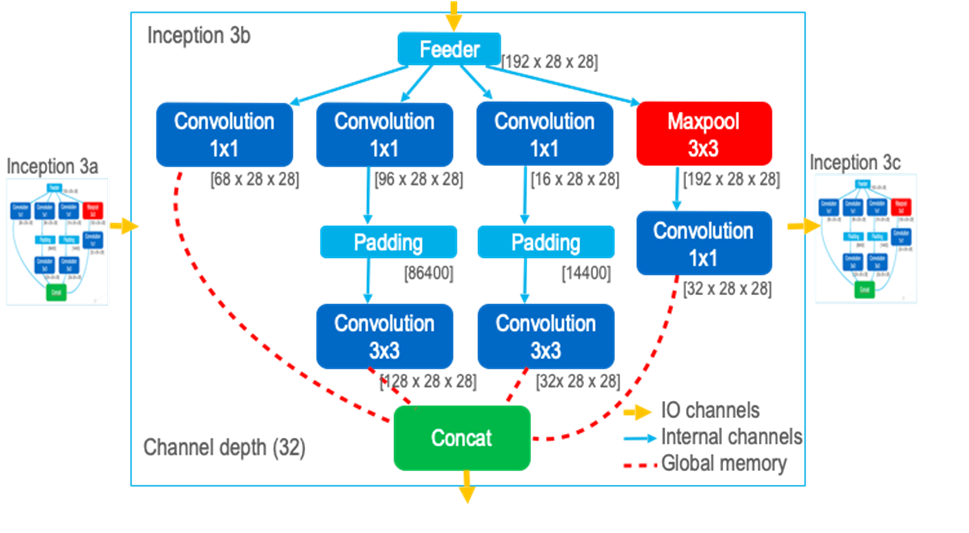
\includegraphics[width=\textwidth,height=\textheight,keepaspectratio]{img/GoogLeNet_Hybrid.PNG}
  \caption{GoogLeNet Hybrid Design}
  \label{fig:GoogLeNet_Hybrid}
\end{figure}

 Figure \ref{fig:GoogLeNet_Hybrid} shows how the internal channels between kernels of the 4 branches and Concat kernel was replaced with global memory. By doing this, we were able to get rid of the stalling problem which we faced in the "pure channels" version of the design.
 
 The global memory access between Concat and the kernels feeding to it required us to modify our plug-in code to launch Concat kernel in one of the four command queues of its feeders. We chose to launch Concat kernels on the same command queue as the 3x3 convolution of branch1. We had to call "clFinish()" for the command queues on which the terminal kernels of each branches were being launched before launching Concat kernel. This way we ensured that the Concat kernel worked on valid data from all the four branches.
 
 Having removed the stalling problem, we trained our sights on executing this design on ten FPGAs. This version of the design took 1.85 seconds to get executed ! The run time of this design is shown graphically in Figure \ref{fig:GoogLeNetHybrid_Runtime_Graph}.
 
 \begin{figure}[!htb]
  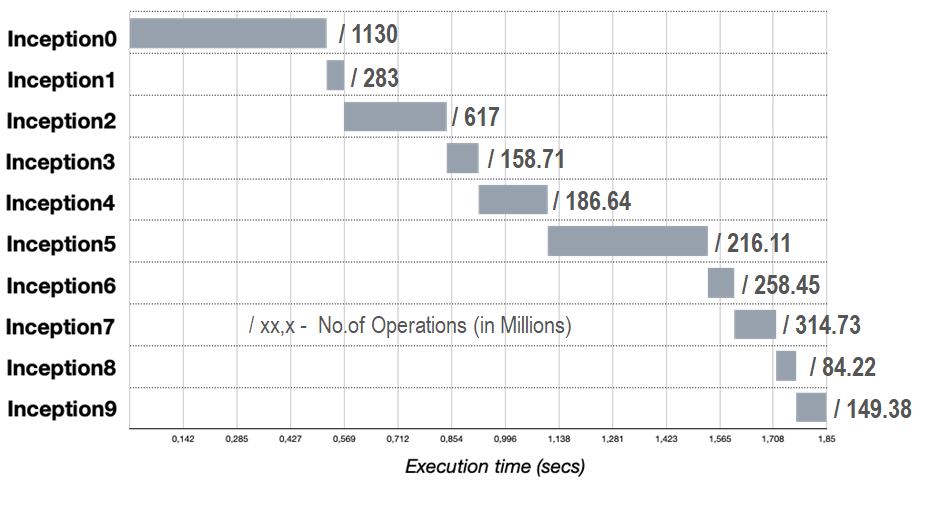
\includegraphics[width=\textwidth,height=\textheight,keepaspectratio]{img/GoogLeNetHybrid_Runtime_Graph.png}
  \caption{Execution time - GoogLeNet Hybrid Design Version 1}
  \label{fig:GoogLeNetHybrid_Runtime_Graph}
\end{figure}

Figure \ref{fig:GoogLeNetHybrid_Runtime_Graph} also indicates that the number of operations in this design in every kernel file is between the number of operations in baseline and DSP usage optimized designs. This is because a lot more optimizations were applied in DSP usage optimized design when compared to hybrid design. In terms of optimizations applied, hybrid falls in between DSP usage optimized and baseline designs.

By analyzing the profile.mon files, we realised that the design could have run faster if not for the bottleneck kernel files of inception0, inception2 and inception5.

To make this design faster, we decided to optimize inception0, inception2 and inception5 files. We referred to the profiling data of these kernel files to find out the bottlenecks within these files. For example, when we analysed the profile.mon of inception2 (3c module), we observed that the slowest branch (out of the 4 branches) was causing that part of the design run slowly. This can be observed from Figure  \ref{fig:GoogLeNet_Hybrid_Before_Opt}. 

 \begin{figure}[!htb]
  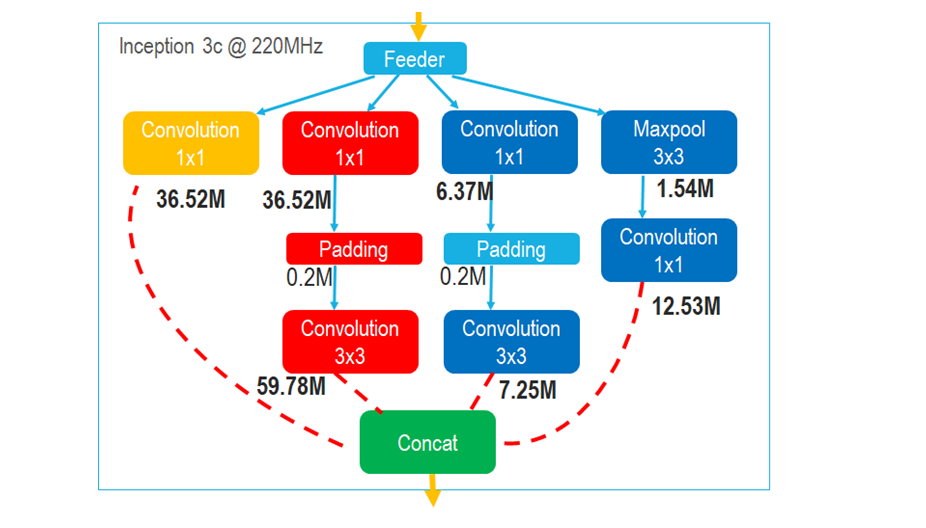
\includegraphics[width=\textwidth,height=\textheight,keepaspectratio]{img/GoogLeNet_Hybrid_Before_Opt.PNG}
  \caption{Number of clock cycles taken by kernels of different branches in inception2(3c) before resource redistribution}
  \label{fig:GoogLeNet_Hybrid_Before_Opt}
\end{figure}


As can be seen from Figure  \ref{fig:GoogLeNet_Hybrid_Before_Opt}, branch1,highlighted in red, requires about 96.5 million clock cycles to get executed - about three times slower than the next slowest branch.  With this design, this part of the design operated at a clock frequency of 220MHz.

We decided to make the kernels in branch1 faster by allocating more resources to it. The resources needed to make branch1 faster had to be taken away from the solitary kernel in branch0 for two reasons : 
\begin{itemize}
    \item the kernel in branch0 was under-performing. Even with a significant amount of resources allocated to it, it was performing relatively slow. In other words, the measured number of operation per cycle was less than the estimated number of operations.
    \item it is the only kernel in its branch. Rearranging the resources in branch2 and branch3 could have complex side effects.
\end{itemize}

When the resources were redistributed to make branch1 run faster, we noticed that the design got synthesized to run at a higher clock frequency - 285MHz. Compared to the previous design, this was an improvement of 65MHz. When we executed this modified design on hardware, we noticed that the run time went down for this particular bitstream. The analysis of profiling data of this new kernel file revealed that we were indeed able to reduce the run time of branch1. This can be seen from Figure \ref{fig:GoogLeNet_Hybrid_After_Opt} where we have documented the number of cycles needed for all the branches to get executed after the redistribution of resources.  

 \begin{figure}[!htb]
  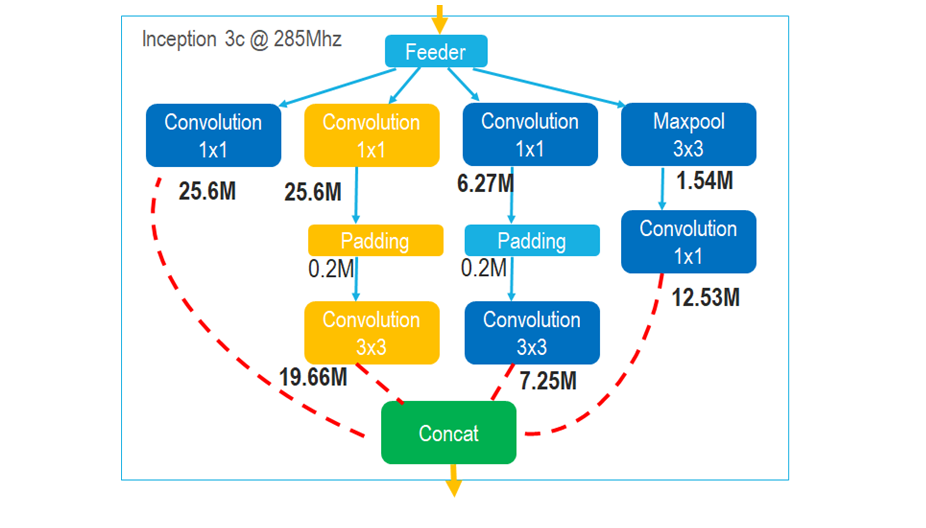
\includegraphics[width=\textwidth,height=\textheight,keepaspectratio]{img/GoogLeNet_Hybrid_After_Opt.png}
  \caption{Number of clock cycles taken by kernels of different branches in inception2(3c) after resource redistribution}
  \label{fig:GoogLeNet_Hybrid_After_Opt}
\end{figure}

The kernels of branch1 have been highlighted in yellow in Figure \ref{fig:GoogLeNet_Hybrid_After_Opt}. The number of clock cycles needed by branch1 to finish execution is about 45 million. This is twice as fast as the previous design. This reduction in required clock cycles and the increase in Fmax(clock frequency) meant the total run-time reduced by a fair margin.

We applied the same kind of optimizations on the other kernel files and the design took 1.18 seconds to classify one image. The relevant performance modeling parameters have been tabulated in Table \ref{tab:GoogLeNetHybridPerfModel}.


\begin{table}[!htb]                          
 \centering
  \captionsetup{
 justification = centering
}
\caption{GoogLeNet Hybrid Design Performance Model}
    \begin{tabular}{|c|c|}
    \multicolumn{2}{c}{\textbf{}} \\ \hline

     Number of Operations    &   3.3 Billion \\ \hline
      Global Memory transfers &   1.9 GB            \\ \hline          
      Execution time    &  1180 ms    \\ \hline
      Operations/second   &   2.79 GOPS \\ \hline
      Operations/cycle &   12.15             \\ \hline
      Operations/byte       &   1.74 \\ \hline
      Global Memory/second & 1.6 GBps  \\ \hline

    \end{tabular}
    \label{tab:GoogLeNetHybridPerfModel}                            

\end{table} 


Throughput, as defined in Chapter \ref{chp:Metrics}, for this design is 0.84 images classified per second. Since accuracy of the model is the same as the one given in the literature (89.9\%), the only factor that could change when calculating Rate Correct Score is the latency. Similar to the other design design, Rate Correct Score is calculated as the ratio between accuracy from literature and the latency of our implementation of GoogLeNet. For this design it is 76.18 per second.

Due to the usage of channels in this design, the memory accesses done through global memory is about 2.5 times less than the DSP usage optimized design. 

In Table \ref{tab:GoogLeNetHybridPerfModel12}, we have tabulated the "inception module" wise break down of performance for the final hybrid design. As can be seen from this, we see a big variation in the fmax (maximum clock frequency) across these individual bitstreams. The best performance (in terms of Operations/cycle) is seen in Inception0 (3a). 
  
In conclusion, we were able to create and execute different versions of GoogLeNet over multiple devices. We strongly believe we could have made our designs much better in terms of latency and throughput. During the last phase of the project, we were able to map out some future tasks to make our designs faster. These insights are discussed in Chapter 
\ref{chp:FutureTasks}.
\begin{table}                          
 \centering
  \captionsetup{
 justification = centering
}
\caption{GoogLeNet Hybrid Design Performance Model}
    \begin{tabular}{ | m{5em} | m{1.5cm}| m{2cm} | m{2cm}| m{2cm} | m{2cm}| m{2cm} | m{2.2cm}| m{2.2cm} | }
    \multicolumn{7}{c}{\textbf{}} \\ \hline

     Inception modules    & fmax (MHz) & Execution time(ms) & DSPs (max. 5760) & Number of operations & Operations/ second & Operations/ cycle \\ \hline
      Inception0 &   259.51  &  523 & 43 & 1.13G & 1.822G & 8.5        \\ \hline          
      Inception1    &  242.01 & 45.06 & 57 & 283M & 1.7G & 7.97  \\ \hline
      Inception2   &   285.95 & 116 & 41 & 617M & 0.96G & 4.5\\ \hline
      Inception3 &   233.53   & 85 & 30 & 158.71M & 836M & 3.88\\ \hline
      Inception4 &   225.17 & 185 & 30 & 186.64M & 0.4305G & 2.0019\\ \hline
      Inception5 & 203.7 & 203 & 30 & 216.11M & 0.1429G & 0.6648 \\ \hline
      Inception6 & 207.08 & 70 & 30 & 258.45M & 1.2425G & 5.7778 \\ \hline
      Inception7 & 240.33 & 111 & 30 & 314.73M & 1.0834G & 5.0381 \\ \hline
      Inception8 & 199.04 & 52 & 30 & 84.22M & 0.5701G & 2.6511\\ \hline
      Inception9 & 184.91 & 86 & 33 & 149.38M & 0.7041G & 3.2743\\ \hline
            Total & - & 1180ms & 354 & 1971M & 1.86 & 8.66\\ \hline

    \end{tabular}
    \label{tab:GoogLeNetHybridPerfModel12}                            

\end{table} 





\newpage
\section{ResNet-50}
The next CNN model we implemented was ResNet-50. While there are more deeper versions of ResNet present the sheer workload of executing them was too much. ResNet-50 was deep enough to achieve the objective of scaling as stated in the project goals. During the implementation of GoogleNet we came across some unforeseen roadblocks which took time to be resolved. However, the team was quick to rectify the mistakes from the lessons learned during previous implementation. This enabled the team to execute several versions of ResNet-50 ranging from the baseline architecture to a more optimised and faster version of the model at a faster pace than before.
We were able to implement four versions for ResNet-50:
\begin{itemize}
    \item ResNet Baseline
    \item ResNet Opt-V1
    \item ResNet Opt-V2
    \item ResNet Opt-V3
\end{itemize}

\subsection{ResNet Baseline}
The method to implement ResNet-50 was very similar to that of GoogleNet baseline architecture. We first generated all the kernel files that were needed to execute the ResNet-50 architecture. After the generation of the kernel files we observed that the number of kernels generated by TVM was less than what our OpenVINO IR was expecting. The reason for this is that in the ResNet-50 architecture there are many of the kernel files whose dimensions are exactly the same. So TVM does not generate the duplicate kernels and only generates the kernels which are not same. This behaviour was opposite to what we saw in GoogleNet where TVM generated more kernels than what was expected. This warranted some extra efforts apart from some pre-optimization tasks that were done to execute the baseline version.
Some of the mandatory modifications done were:
\begin{itemize}
    \item renaming kernel names to match with OpenVINO IR
    \item merging ReLUs with convolutions
    \item removing transpose kernels
    \item duplicating the required kernels not generated by TVM
\end{itemize}
 After the completion of these pre-execution steps the modified code was complied to run on FPGA emulator for Intel Stratix 10 using the latest toolchain-19 of the Board Support Package. Again the functional correctness was checked by comparing the output of our design with the output from TensorFlow implementation. Our modified ResNet-50 code was functionally correct and gave us the right score and label for the image we fed to it. The next obvious step for us then was to implement this baseline version on actual Intel Stratix 10 FPGAs.
 \newline
 In doing so we first looked into the initial report of the entire ResNet-50 architecture which was just a single file. The report, as shown in Figure \ref{fig:ResNet50_baseline_report}, indicated that it is impossible to execute the baseline version on just a single FPGA since our design surpassed the available resources present on the board. This was expected and warranted us to divide the entire architecture into smaller executable parts.
 
 \begin{figure}[!htb]
  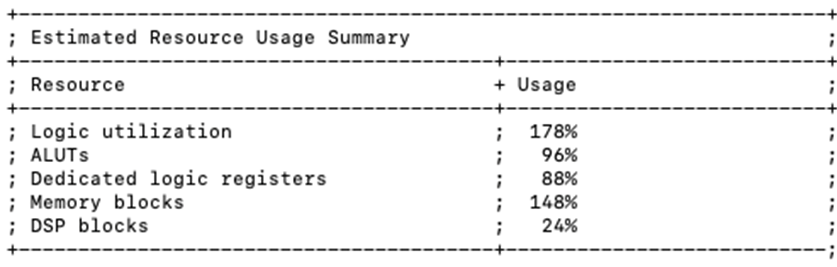
\includegraphics[width=\textwidth,height=\textheight,keepaspectratio]{img/ResNet_baseline.png}
  \caption{Resource Summary - ResNet-50 Baseline Architecture}
  \label{fig:ResNet50_baseline_report}
\end{figure}

We made use of inherent logical divisions present in the ResNet-50 architecture in form of blocks. The entire topology was divided into 5 blocks namely from block1 - block4 with 4 block consisting of 3 units and 1 block consisting of 4 units. The end of each unit was marked by a eltwise kernel which was used as a separation criterion. So at the end of every $3^{rd}$ unit for block1, block3\_1, block3\_2 and block4 a block was formed and block2 was formed at the end of its $4^{th}$ unit. We planned on scaling it to 5 FPGAs with each FPGA being allocated to a  single block. 
After the division of the entire topology into 5 blocks we did not exceed resource utilization requirement and were able to generate the bitstreams and execute it on FPGAs. Since the flashing logic was developed during GoogleNet implementation phase, we adopted the same logic and code with changes in the parity calculations as we were flashing only 5 bitstreams and not 10.   

Global memory was used for intra-node communication and MPI was used to transfer data from one node to another. Here the MPI\_Send() was called at the last of block2 and block3\_2 eltwise kernel except for the last block. MPI\_Recv() was called at the beginning of block3\_1 and and block4.

\begin{figure}[!htb]
  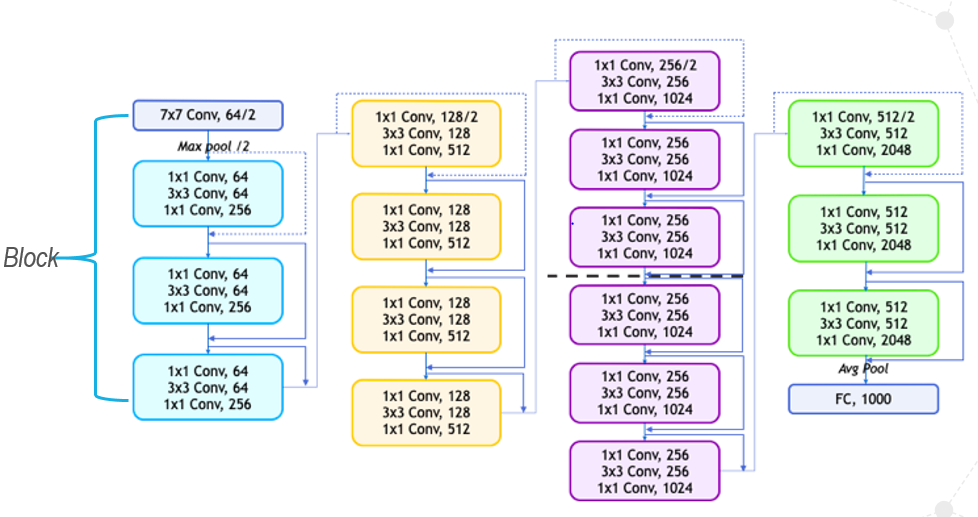
\includegraphics[width=\textwidth,height=\textheight,keepaspectratio]{img/ResNet_division.png}
  \caption{Division of ResNet-50 Baseline Architecture}
  \label{fig:ResNet50_baseline_division}
\end{figure}


One thing to note here is that the baseline version does not contain any kind of optimizations. Practically it is a good practice to pipeline all the loops and bring all II to 1, we chose to execute this out-of-the-box design to gain insights on its performance measure.
As expected the baseline was slow and took 117.34 seconds to classify a single image. The run-time performance of this design can be visualized from Figure \ref{fig:ResNet50_baseline_time}. This is a very slow design and needs to be optimised. However, this design served as a reference point for future comparison on the performance gains which will be achieved with optimised designs.

\begin{figure}[!htb]
  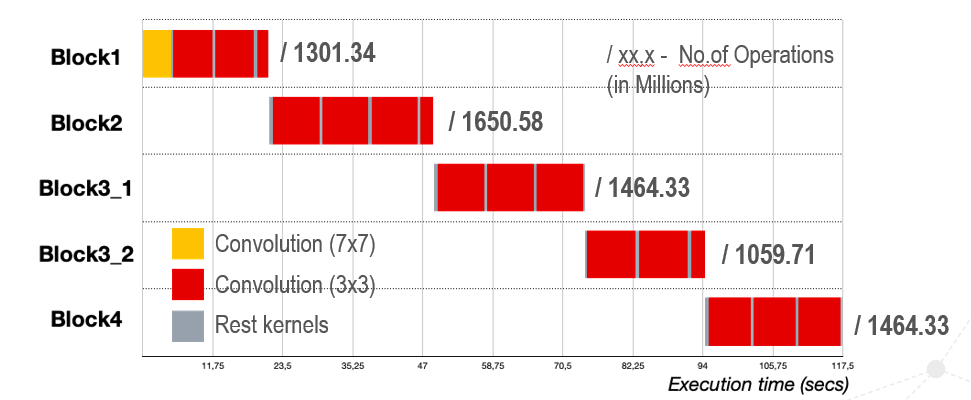
\includegraphics[width=\textwidth,height=\textheight,keepaspectratio]{img/ResNet_baseline_execution.png}
  \caption{Execution time - ResNet-50 Baseline Architecture}
  \label{fig:ResNet50_baseline_time}
\end{figure}


\begin{table}[]
\centering
\captionsetup{
justification = centering
}
\caption{ResNet-50 Baseline Performance Model}
\label{tab:ResNetBaselinePerformanceModel}
\begin{tabular}{|c|c|}
\hline
Number of Operations     & 6.94 Billion \\ \hline
Global Memory transfers & 65.90 GB     \\ \hline
Execution time             & 117345 ms    \\ \hline
Operations/second    & 0.23 GOPS    \\ \hline
Operations/cycle     & 0.29         \\ \hline
Operations/byte      & 0.09         \\ \hline
Global Memory/second    & 576 MBps     \\ \hline
\end{tabular}
\end{table}

We learned that most of the execution time was being spent in 3x3 convolution kernels. Optimising these kernels was a priority. Also due to large II and loop carried dependencies the number of clock cycles needed to execute these kernels was very high. Another factor that contributed to the slow execution was the under-usage of DSP blocks. Less than 1\% of DSP blocks were being used. Since it is the baseline version, no loop unrolling was implemented which could effectively increase the number of MAC operations executing in a single cycle. Due to this at most two MAC operations would be executed in theory. However, looking into the profiling data provided by the respective profile.mon files of each block we observed that our kernels had very less occupancy on FPGAs for raw kernel execution and low read/write efficiency from global memory. The suspected reason for such low efficiency was random global memory accesses by our kernels. So optimising our memory access pattern was also a crucial step in moving forward. Because of all of these factors the measured value which was 0.16 ops/cycle was way less than the 2 ops/cycle estimate. The performance model for this design has been tabulated in Table \ref{tab:ResNetBaselinePerformanceModel}.  
Throughput, as defined in Chapter \ref{chp:Metrics}, for this design is 0.008 images classified per second. Since  the Top-5 accuracy of the model is the same as the one given in the literature (93.29\%), the only factor that could change when calculating Rate Correct Score is the latency. And for this case , Rate Correct Score is calculated as the ratio between accuracy from literature and the latency of our implementation of ResNet-50. This comes to be  0.79 per second.
\newline
Reasons for poor performance of baseline version are:
\begin{itemize}
    \item II greater than 1 
    \item No loop pipelining
    \item Inefficient global memory access patterns
    \item Low DSP usage
    \item Due to serial architecture FPGAs are idle most of the time
\end{itemize}
To summarize the baseline version was very slow and needed to be optimised.

\subsection{ResNet Opt-V1}
The performance of the baseline version was not acceptable and in real world scenarios the latency time was too high to be used. Therefore, there was a need to optimise the baseline version. As mentioned in the previous section the baseline version was completely devoid of any kind of optimization and the major bottleneck was the 3x3 convolution kernel which were responsible for high execution time. Also from the profile.mon file of the kernels from the baseline version as seen in Figure \ref{fig:ResNet50_baseline} the team learned that kernels had very less occupancy on FPGA and also the read/write efficiency was also very less. Optimising and increasing the efficiency and occupancy was one of the main objectives of this optimization phase. The optimization queue had the following tasks:
\begin{itemize}
    \item Loop pipelining
    \item Loop unrolling
    \item Using local memory 
    \item Use of temporary variables
\end{itemize}

\begin{figure}[!htb]
 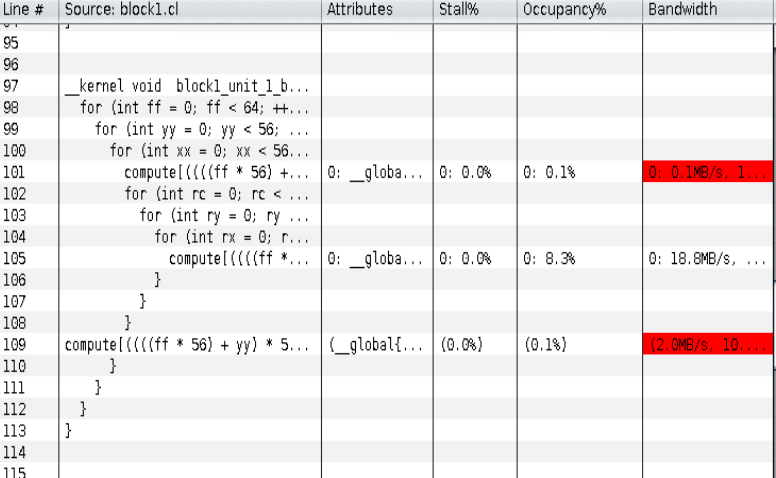
\includegraphics[width=\textwidth,height=\textheight,keepaspectratio]{img/Baselinebottleneck.png}
 \caption{ResNet Baseline Bottleneck Analysis}
 \label{fig:ResNet50_baseline}
\end{figure}

The block-wise divided design was taken to carry out the above mentioned optimizations. All the weights and biases were stored in local memory. Since the sizes of weights and biases were small, storing them in local memory was feasible. This reduced the effort to read everything from the global memory thereby helping in reducing the overall read/write time. Also with the introduction of temporary variables to store the intermediate results getting rid of loop carried dependencies became easy. Furthermore, wherever possible loop unrolling was carried out to increase instruction level parallelism. All of these optimizations resulted in a kernel design in which all the loops were pipelined and it was possible to execute multiple operations in every clock cycle.
\newline
The resource utilization after carrying out these optimizations as seen in Figure \ref{fig:ResNet50_optv1_usage} was under the allowed capacity. One thing to observe is that even though the utilization of the memory blocks increased significantly it is not a true measure of performance metric. Also the DSP utilization is about 2\% which is less and needs to increased. However, it was to be seen how the kernels performed after these set of optimizations and therefore increasing DSP utilization was given low priority at this stage.

\begin{figure}[!htb]
 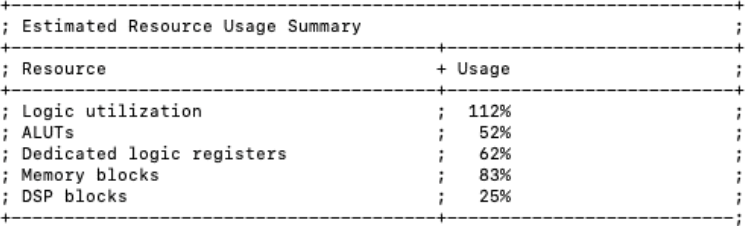
\includegraphics[width=\textwidth,height=\textheight,keepaspectratio]{img/resnetv1ru.png}
 \caption{Resource Summary - ResNet-50 Opt-V1 Architecture}
 \label{fig:ResNet50_optv1_usage}
\end{figure}

After successful functionality testing, bitstreams for all the kernel files were generated and the design was executed on 5 FPGAs. There was a significant increase in performance gain and the entire topology executed in 10.77 seconds. The performance gain was 10$\times$ as compared to the baseline version. This increase in speed was significant and goes to show how loop pipelining and unrolling can have significant impact on performance of a kernel.
\newline
Now the profiling data of these kernel files were analysed. After closer observation of the profile.mon data, we noticed that the occupancy and efficiency parameters, which were crucial in deciding the run-time, had improved. The kernels had high occupancy i.e they spend more time on computation and also the clock frequency of these kernels improved from the previous version. The graph in Figure \ref{fig:ResNet50_optv1_execution} gives the division of the entire run-time. In the baseline version, the run-time for Block1 was around 23 seconds whereas in ResNet Opt-V1, run-time for Block 1 was around 2 seconds. In similar manner all other blocks showed speed-ups in execution time. The entire performance model for this design is tabulated in Table \ref{tab:ResNet50OptV1PerformanceModel}.  

\begin{table}[!htb]
\centering
\captionsetup{
justification = centering
}
\caption{ResNet-50 Opt-V1 Performance Model}
\label{tab:ResNet50OptV1PerformanceModel}
\begin{tabular}{|c|c|}
\hline
Number of Operations     & 7.6 Billion \\ \hline
Global Memory transfers & 13.29 GB    \\ \hline
Execution time             & 10777 ms    \\ \hline
Operations/second    & 6.57 GOPS   \\ \hline
Operations/cycle     & 37.73       \\ \hline
Operations/byte      & 5.32        \\ \hline
Global Memory/second    & 1.234 GBps  \\ \hline
\end{tabular}
\end{table}


Throughput, as defined in Chapter \ref{chp:Metrics}, for this design is 0.09 images classified per second. Since  the Top-5 accuracy of the model is the same as the one given in the literature (93.29\%), the only factor that could change when calculating Rate Correct Score is the latency. And for this case , Rate Correct Score is calculated as the ratio between accuracy from literature and the latency of our implementation of ResNet-50. This comes to be  8.66 per second.

In this version, as we can see from the graph shown in Figure \ref{fig:ResNet50_optv1_execution}, the bottleneck were 1x1 convolution kernels as opposed to 3x3 convolution kernels in the baseline version. The occupancy of these 3x3 kernels was around 99\% with better clock frequency. These set of optimizations solved the major problem which was prevalent in the baseline version. 

\begin{figure}[!htb]
 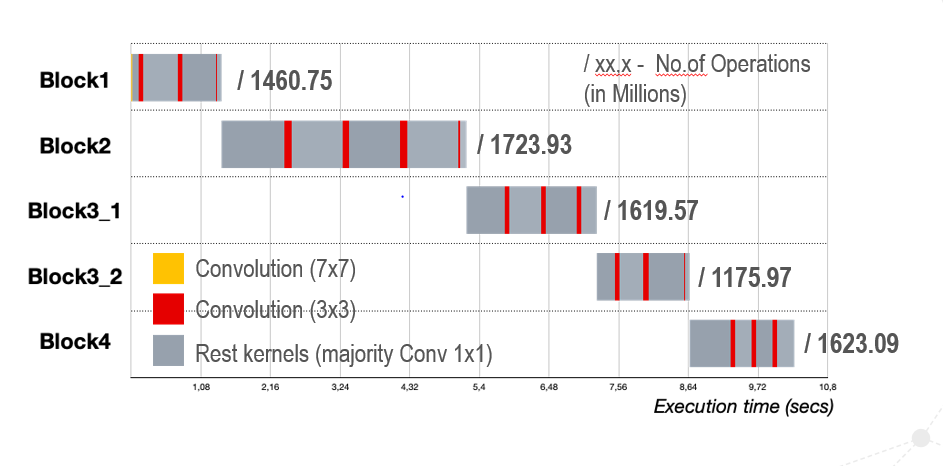
\includegraphics[width=\textwidth,height=\textheight,keepaspectratio]{img/resnetv1exe.PNG}
 \caption{Execution Time - ResNet Optv1 }
 \label{fig:ResNet50_optv1_execution}
\end{figure}

As mentioned earlier DSP blocks were under utilized and increasing it was an imperative step. This warranted a completely different design than what was being executed till now. This resulted in the next version namely ResNet Opt-V2 which will be discussed in the following section.



\subsection{ResNet Opt-V2}
The optimizations performed on the baseline architecture proved to be very effective and provided great result. The performance gain was 10$\times$ from the baseline version. Despite having a promising result there was an opportunity to optimise it further and get a better result. The main reason to go forward with another iteration of optimisation was due to low utilization of the available resources on the board, especially the DSP blocks. Even with the Opt-V1 version the amount of DSP blocks that were used was at most 2\% and the rest was used by the BSP. The main objective of this iteration was to increase the DSP utilization by a significant percentage as an increase in DSP will result in execution of more operations in a single clock cycle. In the previous version of ResNet-50 at most 84 operations per cycle or on an average 15 operations per cycle were being executed due to partial unrolling.
\newline
Till now the topology was divided block-wise with each block containing certain number of units. However, there was a need to completely unroll the inner loops if more DSP blocks were to be used. The current division did not allow that to happen. Therefore, there was a need to divide the entire topology in a completely different way. The next step was to divide it unit wise since the units in itself were very small and allowed for further optimizations. The unit-wise division led to creation of 16 units which will be flashed on 16 FPGAs as opposed to 5 FPGAs from Opt-V1 version. This also led to changes in the Open VINO FPGA plugin since it had to be adapted to the new unit-wise division. The parity calculation for flashing the aocx needed to be modified. The team estimated that there will be significant increase in performance gain of the kernels by increasing the utilization of the DSP blocks and flashing on more FPGAs. 
\newline
The team adopted the strategy implemented during the GoogleNet DSP Usage Optimized phase. The idea was the same. All the operations were executed in the spatial dimension first and then one channel deeper. This happens till all the pixels are operated upon. At this stage the innermost loops were fully unrolled. This resulted in two things. One, the DSP utilization was increased to almost 50\% and second, FPGAs do not have to have to wait for the entire data to be read which would further decrease the kernel execution time. The weights and biases were also copied to local memory reducing global read/write accesses. It was estimated that more than 100 operations per cycle would get executed. 
\begin{figure}[!htb]
  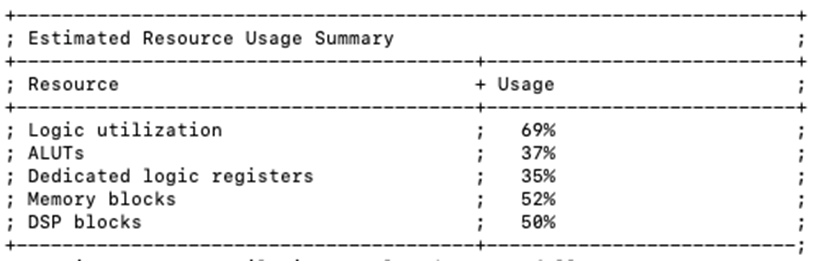
\includegraphics[width=\textwidth,height=\textheight,keepaspectratio]{img/ResNet_DSP_usage.png}
  \caption{Resource Summary - ResNet-50 Opt-V2 Architecture}
  \label{fig:ResNet50_Optv2_usage}
\end{figure}
\newline
When this design was sent for synthesis, as expected the synthesis failed either during the fitter placement or fitter routing phase. Just like GoogleNet we had to reduce the number of DSP blocks being used and send it again for synthesis. However, after reducing the DSP percentage once or twice the kernels were being synthesized. After generation of all the bitstreams the topology was executed on 16 FPGAs and the run-time was 16.49 seconds. Figure \ref{fig:ResNet50_Optv2} shows the run-time of all the 16 units.

\begin{figure}[!htb]
  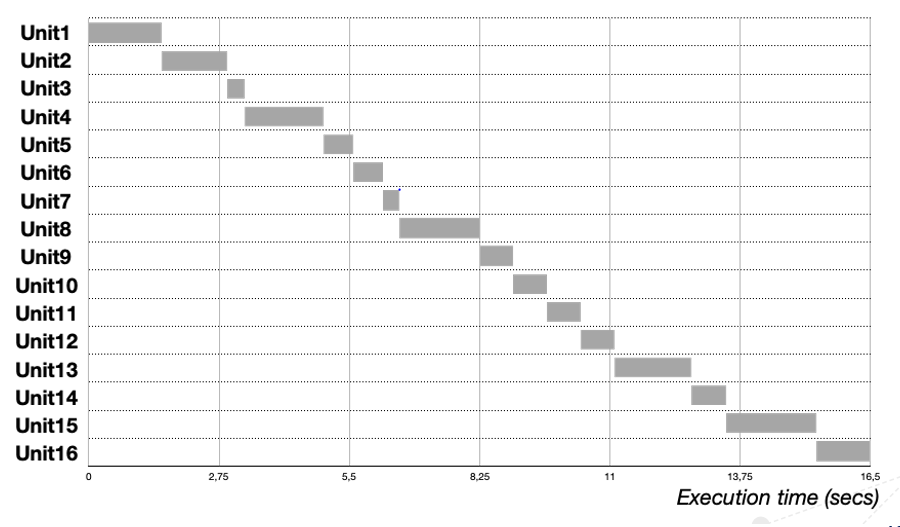
\includegraphics[width=\textwidth,height=\textheight,keepaspectratio]{img/ResNet_DSP.png}
  \caption{Execution time - ResNet-50 Opt-V2 Architecture}
  \label{fig:ResNet50_Optv2}
\end{figure}

According to the estimations the entire topology with this new design should have completed its execution in under 1 second. However, this was not the case and needed deeper investigation to find out the root cause of the problem. When the profiling data of these units were analysed it was found that even though the performance of some of the kernels got better, many of the kernels did not perform as expected. There were two reasons for that:
\begin{itemize}
    \item Stalling problem 
    \item Memory dependency
\end{itemize}
This problem was similar to what we had previously encountered with GoogleNet for the same optimised DSP design. Here the stalling percentage was more than 66\% and the occupancy for raw kernel execution was less on FPGA. At this stage the resource utilization was not high but due to synthesis problem there was no more room to optimize it further i.e perform more loop unrolling to block of code where the image slices are being read. Also the time to synthesize a single kernel file was more than 12 hours on average. This severely limited our opportunities for more optimizations. 
\newline
Due to the above mentioned reasons and the kernel computation logic scaling to 16 FPGAs did not perform the way it was expected to perform. Also due to the synthesis problems and time constraint to meet the project deadline the team could not afford to spend more time on this version of ResNet-50. There was a need to find a new way to optimise these kernels in a way that will increase the execution performance. Therefore, the team decided to execute one more version of ResNet-50 in hope to have better performance gain which resulted in ResNet Opt-V3.
\subsection{ResNet Opt-V3}
In ResNet Opt-V2 the performance of the overall topology was not optimal. There were stalling and memory dependency problems which needed to be resolved. The team needed time and resources to solve this. However, the team was bounded by two constraints: 
\begin{itemize}
    \item Project deadline 
    \item Unavailability of Noctua Infrastrcture due to maintanence 
\end{itemize}
By the time execution of ResNet Opt-V2 was finished the team had very less time of approximately 6-7 days to do any kind of modifications to the existing design and synthesize it again. To our dismay the date of the of the project deadline and maintenance of the Noctua infrastructure conincided which left us with less time to do any kind of optimisation. ResNet Opt-V2 had a runtime of 16.49 seconds whereas ResNet Opt-V1 had runtime of 10.77 seconds. Therefore, the team decided to optimize the ResNet Opt-V1 further as it had shown promising result till now. The idea of optimising it further was taken from the ResNet Opt-V2 i.e streching the design to 16 FPGAs. ResNet Opt-V3 was an amalgamation of the previous two optimization efforts. 
\newline
Here again the entire topology was divided into units instead of blocks. The computaton logic was same as that of the ResNet Opt-V1 i.e the operation takes place in depth dimension first and then spatially. Since this was a unit-wise division there was room to perform loop unrolling. The kernels were pipelined and no extra efforts was needed in that respect. In this version it was possible to fully unroll the innermost loops which were partially unrolled due to resource constraint in ResNet Opt-V1. Optimization priority was given to those kernels which had under performed in the ResNet Opt-V1 which were the 1x1 convolution kernels. 
\newline
Most of the complete loop unrolling took place in the 1x1 convolution kernels. However not every 1x1 convolution kernel was completely unrolled. Every unit consisted two of these slow 1x1 convolution kernels. At any given time only one of these two kernels could be completely unrolled at the beginning of the topology since the dimensions of the image were big. If both of these kernel were completely unrolled, it resulted in high resource utilization thereby rendering the kernel file incapable of being synthesized. As the network got deeper and dimensions of the image started getting small in some units it was possible to completely unroll both the 1x1 convolution kernels. While unrolling the innermost loops it was observed that the DSP utilization was also increasing. However, from past experience it was clear that high DSP utilization would result in synthesis failure. Therefore, it was decided to keep DSP utilization under 35\%. In such fashion all the 16 units were optimised, tested and sent for synthesis. 
\begin{table}[!htb]
\centering
\captionsetup{
justification = centering
}
\caption{ResNet-50 Opt-V1 Performance Model}
\label{tab:ResNet50OptV3PerformanceModel}
\begin{tabular}{|c|c|}
\hline
No.of Operations     & 6.96 Billion \\ \hline
Global Mem transfers & 52.18 GB     \\ \hline
Exe time             & 12105 ms     \\ \hline
Operations/second    & 0.535 GOPS   \\ \hline
Operations/cycle     & 2.63         \\ \hline
Operations/byte      & 0.12         \\ \hline
Global mem/second    & 4.31 GBps    \\ \hline
\end{tabular}
\end{table}
After modifying and testing the kernels from ResNet Opt-V1 team had only 4 days to synthesize 16 designs. The timeline was very tight as some of the kernels might take a long time to get synthesized. Four to five designs were put to synthesis in parallel to meet the maintenance deadline. During synthesis some of the designs failed to synthesize and had to be modified again i.e reduce unroll factors. Due to this by the end of the deadline 13 design got synthesized and synthesis of 3 designs namely unit 13, unit 14 and unit 15 was unsuccessful. 
\newline
To execute the entire topology 16 bitstreams were needed. The remaining 3 bitstreams were taken from ResNet Opt-V2. While executing this version of ResNet the plugin was not able to parse beyond the eltwise kernel of 4 units namely unit 3, unit 9, unit 10 and unit 12. The reason for that is unclear as nothing was changed in those kernels. The bitstreams for those 4 units were taken from ResNet Opt-V2. In total there were 9 units from ResNet Opt-V3 and 7 units from ResNet Opt-V2 used to run the network. Therefore ResNet Opt-V3 was a mixture of two version of optimization. 
\newline
It was possible to run the network on FPGA. After successful execution of the network the runtime obtained was 12.105 seconds. This execution time was better than ResNet Opt-V2 but had degraded in comparison to ResNet Opt-V1. 
\begin{figure}[!htb]
  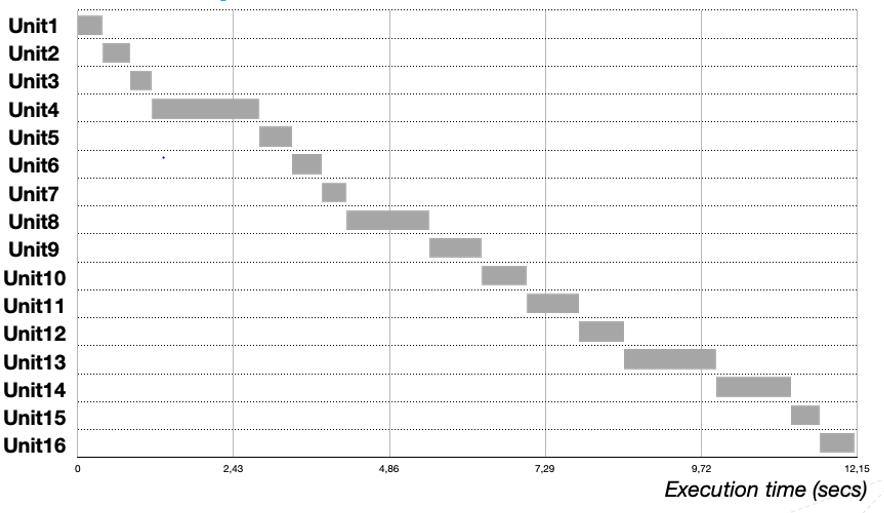
\includegraphics[width=\textwidth,height=\textheight,keepaspectratio]{img/ResNet_OptV3_execution.png}
  \caption{Execution time - ResNet-50 Opt-V3 Architecture}
  \label{fig:ResNet50_Optv3}
\end{figure}
Profiling data showed that the performance of units from ResNet Opt-V3 had become better than their ResNet Opt-V1 counterpart. This has been illustrated in Fig \ref{fig:ResNet50_Optv3_kernel}. In this unit the block1\_unit1\_bt\_v2\_conv2\_Conv2D kernel executed in around 400 ms whereas the same kernel took 1.46 seconds to execute in ResNet Opt-V1. This was 3$\times$ performance gain. In similar manner kernels from other units of ResNet Opt-V3 design showed speed up. Due to the usage of 7 designs from the previous ResNet Opt-V2 version the execution time increased as the unit themselves were slow from that version. 
\newline
The main takeaway from this version is that ResNet-50 could have been executed in less 10.77 seconds if only we had all the units completely optimised. However, the team was able to create and execute different versions of ResNet over multiple devices. We definetely could have done much better but the team faced some tough challenges during the entire development phase. These challenges will be discussed in \ref{sec:challenges}

\begin{figure}[H]
  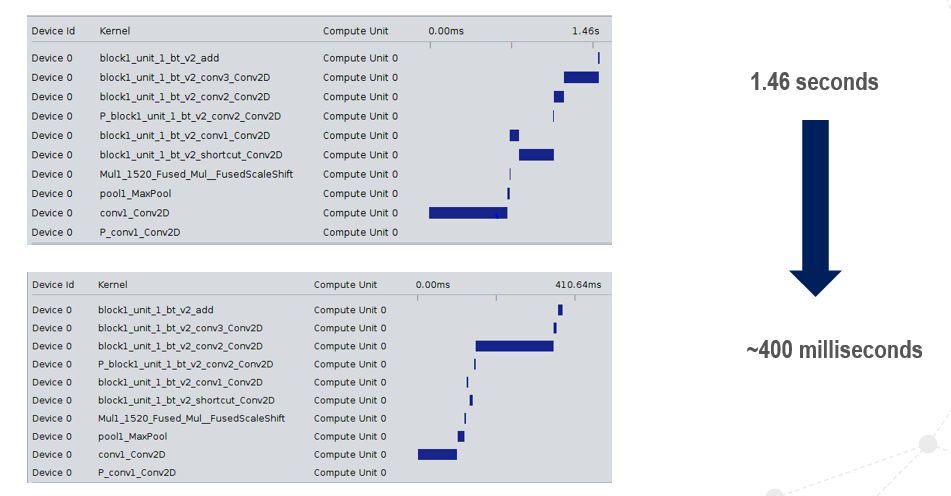
\includegraphics[width=\textwidth,height=\textheight,keepaspectratio]{img/ResNet_OptV3_performance.png}
  \caption{Improvement in performance at kernel level : ResNet50 Optv3}
  \label{fig:ResNet50_Optv3_kernel}
\end{figure}
%End of the chapter
\chapter{Related Work}
A lot of research has been going on in the field of enhancing the computation speed of CNNs on FPGA for quite some time. In this section, we will take a look at the various research work that has been done so far. We know that CNNs consist of different layers such as convolution, pooling, and fully connected layers, out of which convolution forms a major part of it. \cite{DBLP:conf/iccv/LiuLSHYZ17} implemented convolution layer using sequential nested \textit{for} loops. In our project, we are also using sequential nested for loops for the implementation of convolution layer.

We also know that FPGAs and ASICs increase the speed of inference, while GPUs still excel at floating point operations. CNNs generally work on floating-point representation but working with them comes at a cost in the form of computation time. The need of the hour is to have high throughput and high efficiency. Hence it is better to use data in a fixed-point representation. To cite a few, most of the research work of \cite{DBLP:journals/corr/abs-1712-05877}, \cite{DBLP:conf/fpga/QiuWYGLZYTXSWY16}, \cite{DBLP:conf/icassp/ShinHS16} has been done in the field of quantization in order to improve computation speed through low bit representation. \cite{DBLP:journals/corr/CourbariauxBD14} implemented block floating point and their CNN topology gave a 1.0 pp accuracy loss. \cite{DBLP:conf/fpga/QiuWYGLZYTXSWY16} used an 8-bit representation of weights on ImageNet and achieved a 0.4 pp accuracy loss. Similarly, other techniques like binarization, ternarization, etc., are also implemented and these techniques showed better performance than the standard CNN which used FP32 bit representation. In our project, we are trying to quantize weights in 16-bit representation because by doing quantization of weights in 16-bit we will have a mere loss of 0.1pp in accuracy and also it will help us to achieve our goal of high throughput.

In 2018 a survey was carried out which discussed various tool-flows for mapping of CNN on FPGAs. These tool-flows were distinguished into two categories based on the architecture each tool-flow adheres to. First architecture is \textit{Streaming Architecture} where each layer is assigned a hardware block and these layers are chained to form a pipeline\cite{DBLP:journals/tnn/DundarJMC17}. Second architecture is \textit{Single Computation Engine} architecture which is used to form an overlay. Due to this, it provides flexibility, portability, fast configuration time. In our project, we are trying to create overlays, where we will create a separate .aocx file for each layer and then these can be called in the OpenVINO plugin to deploy it on FPGAs.


\chapter{Project Organization}
In this section, we describe how the project was organized and monitored from beginning to completion. This will cover many aspects such as phases in project, planning of timelines, organizational decisions taken in the projects etc. 


\section{Project Phases }
The overall timeline of the project can be divided into three major phases. They are namely tutorial phase, research phase and implementation phase. The first two phases were carried out as a whole and the implementation phase was further divided into sub phases according to software development life cycle.

\section{Tutorial Phase }
The aim of this phase was to introduce the project group to the core topics of the project - programming FPGAs using OpenCL framework, heterogeneous computing,  CNNs, and performance modeling. The project kick off meeting was held on 11th October 2018. After this, the first tutorial session was held on 16th October. Our mentor Dr. Tobias Kenter organized this phase by conducting lectures, giving programming assignments and evaluating each team member’s progress. Along with these, we also learned about CNNs through Stanford’s YouTube lecture series named “Convolutional Neural Networks for Visual Recognition”. 

The programming tasks and the topics covered are as follows : 
\begin{itemize}
\item Task 1 : Writing OpenCL host-side application in Eclipse IDE. Writing and compiling a simple OpenCL kernel (both single work item and NDRange kernel).  
\item Task 2 : Customizing bashrc file, building code using makefile , research about OpenCL channels and pipes.
\item Task 3 : Group task on classification of handwritten digits using Linear Classifier. 
\item Task 4 : Creation of workflow documents which contain the knowledge gained during the tutorial phase. Research about git best practices.
\item Task 5 : Shift Register Optimization
\item Task 6 : Implementing OpenCL channels and widening them. 
\item Task 7 : Group task on classification of handwritten digits using CNN Based Classifier. Performance modeling and optimization of the design.
\end{itemize}

\section{Research Phase}
 
This phase started in the first week of February 2019. During the research phase of the project, the team members conducted background research on 4 frameworks - Intel OpenVINO, Xilinx ML Suite, TVM and Microsoft Project Brainwave. Every week the team members presented short presentations on the findings of the research. We discussed the advantages and disadvantages of these tools to see how they fit into our project plan. After brainstorming, we identified a design that was a combination of TVM and OpenVINO to achieve our goals. The decision points of selecting these tools have been discussed in Chapter \ref{chp:Toolkits}.

\section{Implementation Phase}
In this phase, we followed the activities which are followed in any typical Software Development Life Cycle (SDLC) . These SDLC activities are further divided into sub phases and discussed in the below section. 
\subsection{Project Planning}

In this phase, we decided on the goals, feasibility of achieving these goals, prioritizing and the overall organization of the project . This involved defining the scope, dividing the project into subgroups, assigning roles and responsibilities (such as Team Leader and git master). We decided to use the Waterfall model since our project is a short-term project with linear sequence of phases and goals were defined and fixed already. Here we defined the sub phases and estimated the time required to fulfill intermediate goals. Some of the aspects of planning are further described  below. 

\begin{itemize}
\item \textbf{Scope} : The initial scope of the project was to implement 3 state of the art CNNs (namely GoogLeNet Inception V1,  ResNet-50 and Inception V3). Later we dropped the implementation of the third topology and decided to focus on optimizing the performance of the other two topologies because of time constraints.
\item \textbf{Sub groups} : Team OpenVINO and Team TVM. The OpenVINO team worked on FGPA plugin development. The TVM team worked on generating kernels for selected CNN model and customizing the kernels to suit OpenVINO's IR. 
\item \textbf{Team Leader} : Team Leader was elected by the team members roughly at the beginning of each milestone. This meant that we had more than one Team Leader through the course of the implementation phase. The role of the Team Leader was to identify and create tasks for the project team and assign it to individuals based on skills and their availability. Every weekly meeting was driven by the Team Leader by putting discussion points on the table between our mentor and team members. 
\item  \textbf{Weekly meetings} : Weekly meetings were held twice a week - on Mondays and Wednesdays. Here we discussed the status of the tasks, issues being faced and tasks for upcoming week.
\item \textbf{Minutes of Meeting} : After each weekly meeting, team members prepared MoMs in a round robin fashion. This document contained project organizational updates, progress of tasks, and decisions taken in the meeting.
\item \textbf{Communication} : Communication tools we used in the project are Slack and PG Emailing list.
\item \textbf{Task Tracking} : We used GitLab's Issue board feature to track and manage both tasks and issues in the project. The Team Leader would create tasks after every weekly meeting under suitable labels. The labels are helpful in identifying and classifying tasks in different buckets. The various labels used are OpenVINO, TVM, Documentation, Kernels, optimizations and scrapped. Any task would be go through three stages - open, in progress, closed. Each task has a Description, Deliverable and  Exit Criteria. Upon creation, a task would start off in "open" stage. After this, the assigned team member would take the task and move it into "in progress" stage. In this stage, the team member would update the progress of the task by adding comments and findings. Once the task is completed, it would be moved to "closed" stage. 
\end{itemize}

\subsection{Finalizing the Plan and Mini Presentation}

During this phase, we finalized the tool-flow and gave a short presentation on the final plan. The Audience were PC2 group members and it was presented on 17th April 2019. The outcome of this phase was Project Plan document reviewed by Dr. Tobias Kenter and Project Plan presentation in the form of PowerPoint presentation(PPT file). 

\subsection{Design}
The entire architecture of the project is contained in design document. It is a sequence diagram which shows the interaction between OpenVINO , TVM and users. It also shows the order in which these interactions take place. This document helped us in understanding the bigger picture and we updated it whenever necessary. 

\subsection{Coding and Testing}
The most important phase of our project was this phase and arguably the lengthiest phase. We devised five milestones to achieve our project goals. These milestones were in increasing order of complexity. In this section, we discuss what was planned and achieved in the milestone and also what coding and testing strategies we used. 


\textbf{Milestone 1} : The objective of this milestone was to develop and test an FPGA plugin compatible with Noctua cluster for OpenVINO and generate kernel codes (in order to run Simple CNN
topology on a single FPGA) using Tensor Virtual Machine (TVM) and later customize TVM generated kernels for said plugin and to synthesize the codes for Stratix 10 board. 
The FPGA Plugin was able to launch the kernels on emulation but these kernels were not generated by TVM because our simple CNN was a custom model and not a standard model.  


\textbf{Milestone 2} : The objective of this milestone was running the simple CNN topology on multiple FPGAs available in the Noctua Cluster. We were able to scale the design using external channels on 2 FPGAs. 

\textbf{Breakpoint:} We had planned to achieve Milestone 1 in the first three weeks of April and Milestone 2 by the second week of May. The back up plan in case we failed to meet the above criteria with OpenVINO, was to scrap OpenVINO and go with Xilinx ML Suite as Plan B with a similar design discussed above. 

\textbf{Milestone 3 \& 4:} On completion of Milestone 1 and 2, we had a simple CNN model that could run on 2 FPGAs . The goal of Milestone 3 was to deploy all the three topologies and stretching each of them over multiple FPGAs. This didn't go as planned because of two reasons. 

Firstly, there was a layout mismatch in how TVM was generating the kernels and how OpenVINO generated the IR. This error arose because we were using two different tools which generate different IRs for the same CNN model. Identifying this error and fixing it took a lot of time and we missed to complete the objectives of this deadline. Secondly, when we had stretched the topology over two FPGAs, we didn't use MPI. For stretching over multiple FPGAs, we had to update the plugin with MPI calls. Due to these issues which we didn't anticipate at the time of planning, we found the milestones to be too restrictive and hence we decided to handle the tasks in a "on the fly" basis. And we treated milestones as a reference to keep track of our sub goals. 

After solving the above mentioned issues, we implemented GoogLeNet (Inception V1) and ResNet-50. We came up with performance model to understand shortcomings of the designs. Based on the results of performance modelling, we worked towards bettering our designs.

\textbf{Coding and Testing Strategies} : The team members involved with the development process started the coding tasks by understanding the requirement from Gitlab Issue board. Depending on the type of the task, the members followed various approaches for coding and testing. For example, for an FPGA Plugin development task, developers would code together by understanding complex data structures of OpenVINO and later debugged the code by inserting print statements. Another example can be of kernel optimization tasks, where the developers would first decide on what optimizations to perform, applied the optimization on one functional block of the design, and depending on the effectiveness of such optimizations, would go on to work individually on applying the same optimizations for other functional blocks of the design. 


\subsection{Result collection and Performance Evaluation}
To explain the results we obtained from our CNN topology implementation, in this phase, we came up with various performance models. This was done for each design keeping some of the metrics in mind like execution time, operations per cycle, global memory read and write etc. We analyzed the numbers and started looking into optimization techniques to make the numbers better. After piloting the technique on one or two modules, and checking the new results, we would go back to coding and testing phase again to implement the technique across all the remaining kernels. 

\subsection{Presentation and Final project report}
During this phase, we presented our final project presentation on 23rd September 2019. It covered almost all aspects of project beginning from motivation, introduction to goals , our implementations and results we achieved. Later, the final project report was prepared to explain the implementation and results in detail. 

\chapter{Future Tasks} \label{chp:FutureTasks}
          \item \textbf{ Exploring channel width:} \medskip
    
    Currently the GoogleNet hybrid design uses internal and external IO channels. These channels have specific width and can transfer the amount of data equal to the width of the channel. Due to time constraints the team couldn’t explore different channel width and observe the performance of the design. For future we would like to explore different channel widths to see their effect on performance.
    
     \item \textbf{Batch processing: }\medskip
    
    The OpenVINO plugin that the team has developed classifies one image at a time and gives out the classification result. Since we are classifying one image only we are not efficiently using the FPGAs. For future we would like to classify several images at a time so that FPGAs are not kept idle and used to their full potential.

 \item  \textbf{Solving memory dependency: }   
 
 One of the reasons for sub optimal performance of our design is memory dependencies present in the kernels. This causes serial execution of the loop. We couldn't solve these dependencies due to time constraints.  Future task would be to remove these dependencies with more efficient memory access patterns in the compute logic.  \begin{code}
 \begin{minted}{c++}
for (int rc = 0; rc < 64; ++rc)
       {
           //Store 1 slice of input image
           float image_slice[58*58];
           #pragma unroll 29
           for (int in = 0; in < 58*58; in++){
               image_slice[in] = input0[(58*58*rc)+in];
           }
           #pragma unroll 2
           for (int yy = 0; yy < 56; ++yy)
           {
               #pragma unroll
               for (int xx = 0; xx < 56; ++xx)
               {
                   float temp_0 = 0;
                       //Convultion 3*3
                       float temp_2 = 0;
                       #pragma unroll
                       for (int ry = 0; ry < 3; ++ry)
                       {
                           float temp_1 = 0;
                           #pragma unroll
                           for (int rx = 0; rx < 3; ++rx)
                           {
                               temp_1 +=  (image_slice[((yy+ry) * 58) + (xx) + rx ] * local_weight[(((((rc) * 3) + ry) * 3) + rx)]);
                           }
                           temp_2 +=temp_1;
                       }
                       temp_0 += temp_2;
                       temp_out[yy][xx] += temp_0;
               }
           }
       }
\end{minted}
\caption{Example code with memory dependency. In the code we can see the memory dependency for rc loop.}
\label{code:memory_dependency}
\end{code}\\*At line we are doing load and store operation at the same time due to which this issue arises. The issue is shown in HTML report.   \begin{figure}[H]
  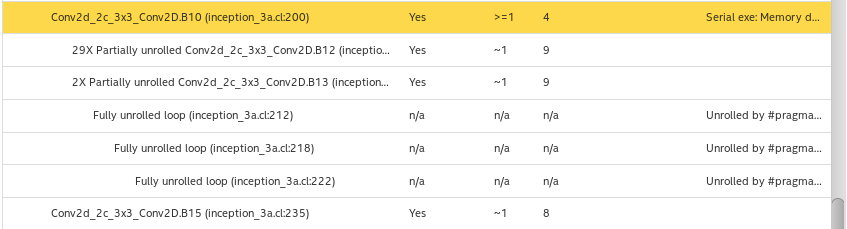
\includegraphics[width=\textwidth,height=\textheight,keepaspectratio]{img/memory_dependency.png}
  \caption{HTML report showing memory dependency in the kernel}
  \label{fig:memory_dependency}
\end{figure}                                                                                    

  \item \textbf{General plugin: } \medskip
    
    Currently the OpenVINO plugin supports only GoogleNet and ResNet topologies. In future we would like to add support for more layers of different CNN networks so that the plugin can launch all different topologies.

       
  



\chapter{Comparison with state-of-the-art benchmarks and challenges faced}

\begin{table}[!htb]
\centering
\captionsetup{
justification = centering
}
\caption{Comparison with state-of-the-art benchmarks}
\begin{tabular}{|c|c|c|c|}
\hline
\textbf{Topology} & \textbf{\begin{tabular}[c]{@{}c@{}}FPGA \\ execution time\end{tabular}} & \textbf{\begin{tabular}[c]{@{}c@{}}OpenVINO CPU  \\ execution time\end{tabular}} & \textbf{\begin{tabular}[c]{@{}c@{}}Microsoft \\ Brainwave\end{tabular}} \\ \hline
GoogLeNet & 1.18 sec  & 8.79 ms & -\\ \hline
ResNet–50 & 10.77 sec & 19.42 ms & 4 ms \\ \hline
\end{tabular}
\label{tab:Comp_benchmarks}

\end{table}
Table \ref{tab:Comp_benchmarks} shows the comparison of execution times of different topologies on different platforms and on a deep learning platform, Microsoft Brainwave. OpenVINO CPU plugin was executed on "cc-frontend" with 16 CPUs, 4 cores in each socket running at an average clock frequency of 1.2 GHz.  OpenVINO FPGA plugin was executed on multiple Intel Stratix 10 FPGAs in the Noctua infrastructure and Microsoft Brainwave executes the CNN topologies on one Stratix 10 FPGA.

For GoogLeNet topology, execution time on OpenVINO CPU plugin was 8.79ms and on OpenVINO FPGA plugin was 1.18s. Microsoft Brainwave does not support this topology. Whereas for ResNet topology, execution time on OpenVINO CPU plugin was 19.42ms, on OpenVINO FPGA plugin was 10.77s and Microsoft Brainwave took execution time of 4ms on 1 FPGA.

 We observed that the difference in execution time of the topologies is very vast between FPGA plugin and CPU plugin. Hence, we examined deep to find out the probable causes for this difference. 

%End of Chapter
\section{Causes of sub-optimal results} 
\label{sec:challenges}

\begin{enumerate}

\item\textbf{Limited parallel operations: } The OpenVINO CPU plugin is highly optimized to run on CPUs. The CPU on which the OpenVINO CPU plugin was run is a multicore system with a maximum operating clock frequency of 3.2GHz. We can infer from this that the OpenVINO CPU plugin was able to exploit the parallelism offered by the multicore systems to execute the design in a highly parallel manner. Approximately, the OpenVINO CPU plugin was able to execute about 55 Operations per cycle.
On the other hand, the best we could do was 12 Operations per cycle for short durations in GoogLeNet hybrid design.

\item\textbf{Serial Execution of the Designs: }
The GoogleNet and ResNet CNN models have a sequential architecture. Since the whole network is too big to fit in one FPGA, we divide the structure into several small sub-structure and then execute them on several FPGAs. Due to sequential architecture, the next sub-structure is dependent on the previous sub-structure, hence the next FPGA has to wait till the previous FPGA completes the execution. 
This problem can be overcome by modifying the design to support batches of images.


\item\textbf{Accumulated Data based logic: }
The kernel design that we have used in GoogleNet hybrid design makes use of internal and external IO channels. These kernels work on accumulated data, i.e., the kernel starts processing after only it has received the complete set of data from the channels. Hence the kernels here are idle till they receive the whole data. One way to solve this issue is to use a streaming design. Streaming design has data pipelined in its architecture thereby eradicating the idle time of the kernels.

\item\textbf{Limited design space exploration: }
Several factors come in to play during the synthesis of kernels. In our design, we observed a positive correlation between the amount of DSP block usage and synthesis time. Due to some of the designs taking upto 24 hours to get synthesized, it was very challenging to iterate over different optimization points. This meant we could not bring to fruition some of the optimization ideas we had in mind.

The design space for applications running on FPGAs is very big. We had no control over the final fmax as this is determined by the compiler. But we noticed a correlation between DSP usage and fmax. If we were too aggressive with increasing DSP usage, then fmax would go down considerably. If not enough DSP blocks were requested for (by not unrolling the compute loops), then we would get a good fmax but compute parallelism would go down. So we had to explore this large design space to find the right balance between DSP blocks and fmax. And we could not really cover much of this design space.


\item\textbf{Lack of Experience: }
The ability to find the right balance between different parameters, to determine the right number of FPGAs to scale over, to debug  stalled kernels etc is something which comes over time. The lack of experience meant we were not able to figure out the best design paradigms to implement different CNNs. On the other hand, the lessons learnt during different design points  helped us accelerate at the later stages of the project. With time and experience, better solutions can be implemented.

\end{enumerate}


\section{Quantization Issues }
One of the initial goals listed in the project plan was to perform Quantization. Quantization involves low precision math and hence can positively impact various performance metrics of our project. This was the motivation behind choosing this subgoal. Among various approaches available to achieve this, after discussion and research, we decided to implement Post Training Quantization which is supported by both TVM and OpenVINO. The Calibration Tool present in the latest release of OpenVINO performs post-training quantization of the CNN model to int8 before the model’s IR is passed on to the inference engine. This task is less time consuming and less complex as we don’t have to retrain the model using quantized weights. Also, we were able to generate kernels using TVM’s quantize function. 

Although most of the aspects seemed to fall into place, we came across two potential risks that hindered us in achieving this goal. 
		
\begin{itemize}
\item The version of OpenVINO used in the project (2018 R5) only supports FP16 or FP32 operations. The Post Training Quantization discussed previously is available in the latest version (2019 R1). This implied that we should migrate our project 2018 R5 version to the new one. During that time of the project, many branches of the repository were simultaneously under development and it made migration difficult. 
\item To support migration to a new version of OpenVINO, we also may be required to make modifications to the existing FPGA plugin and again, this would involve understanding the changes, impact analysis and development. Due to the limited amount of time available, even this affected our decision to stop pursuing this goal.
\end{itemize}

\appendix
\chapter{Appendix}

\section{OpenVINO Model Optimizer}
Model Optimizer is a python based tool which takes a pre-trained CNN model (.pb file) as its input and converts it to an intermediate representation consisting of a .xml file containing the network topology and a .bin file containing the layer weights. This makes the high level training frameworks such as Tensorflow and Caffe independent of the underlying hardware platforms. The steps to generate the IR are as follows:-

\begin{itemize}
    \item Download an available pre-trained CNN model. We have used the slim image classification library models in our project.
    \item The model is available as a single .ckpt file, for which the inference graph needs to be exported in the form of a .pb file.
    \item The model can now be frozen to give a single big .pb file which contains both the topology and the weights of the model.
    \item This frozen model can now be used to generate IR through the  command given in Code \ref{code:Model_opt}.
\end{itemize}

\begin{code}[!htb]
 \begin{minted}[fontsize=\small]{bash}
[user@fe-1 ~]$ python \  
/opt/intel/computer_vision_sdk_2018.5.455/deployment_tools/model_optimizer/mo_tf.py \ 
--input_model ./vgg_19_frozen.pb --input_shape [1,224,224,3] \
--mean_value [127.5,127.5,127.5] --scale 127.5

\end{minted}
\caption{Command to invoke Model Optimizer}
\label{code:Model_opt}
\end{code}

\section{Build Inference Engine Project on CC Frontend.}
\textbf{Software Requirements:}
\begin{itemize}
\item cmake 3.9 or higher
\item gcc 4.8 or higher
\end{itemize}
\textbf{Cloning the DLDT repository:}
We need to clone the open source Deep Learning Deployment Toolkit repository.

\begin{itemize}
\item execute the following command to clone the DLDT repository. \\* \raggedright\texttt{ git@git.uni-paderborn.de:cs-hit/pg-custonn2-2018-3rd-party/dldt.git}   
\item Once the DLDT repository is cloned, we need to clone a sub project \textbf{ade} into the project. Navigate to dldt dir and execute the command \\* \texttt{git submodule init} \\*  followed by \\* \texttt{git submodule update --recursive}. \\* 
\end{itemize}

\textbf{Build Steps:}

\begin{itemize}
\item Navigate to \\* \texttt{cd <dldt>/inference-engine}
\item Create a build directory  \\* \texttt{mkdir build}
\item Inference Engine uses a CMake based build system. In the \textbf{build} directory run the cmake to create the makefile.
\item cmake command \\*  \raggedright\texttt{ cmake3 -DCMAKE\_BUILD\_TYPE=Release -DENABLE\_CLDNN=OFF -DENABLE\_GNA=OFF .. }
\item The above command is by disabling GPU and GNA Plugin, If you want to enable those, please set the arguments to ON
\item Once the cmake command is executed succesfully, run the make command to build the DLDT project. \\* \texttt{make -j16}
\item To switch on/off the CPU and GPU plugins, use cmake options -DENABLE\_MKL\_DNN=ON/OFF and -DENABLE\_CLDNN=ON/OFF.

\end{itemize}

\section{Steps to run GoogLenet using OpenVINO FPGA Plugin with MPI on Stratix 10 FPGAs}
\textbf{Connecting the Noctua Cluster}
\begin{enumerate}
\item Connect to the Noctua Load Balancer \\*  \raggedright\texttt{ssh fe.noctua.pc2.uni-paderborn.de} \\*  (This command can be executed from the CC Fe also)
\item Connect to Noctua FPGA front nodes \\* \raggedright\texttt{ssh noctua}
\item Load OpenMPI,CMake and GCC modules \\* \raggedright\texttt{module load intel/18.0.3} \\*  \raggedright\texttt{module load mpi/OpenMPI/1.10.3-GCC-5.4.0-2.26} \\*  \raggedright\texttt{module load intelFPGA\_pro/19.1.0 nalla\_pcie/19.1.0 gcc/6.1.0} \\*  \raggedright\texttt{module load devel/CMake/3.6.1-foss-2016b} \\*  The above procedure has to be followed each time you login to Noctua node.
\end{enumerate}

\textbf{Build the OpenVINO noctua plugin containing MPI :} OpenVINO noctua plugin is built to integrate IR from Model Optimizer with OpenCL Kernels generated from TVM and launch these kernels on multiple FPGA's using MPI send and receive functions .

We have created a GitLab Tag  \texttt{custonn2}  for the dldt project with the custom  FPGA plugin. Please switch to this tag or clone this tag if you are in different branch.

If you are building the Inference Engine for the first time , please refer to the section A.2. 
\begin{enumerate}
\item Navigate to build directory of OpenVINO inference engine: \\*\texttt{cd \$<dldt>/inference-engine/build}
\item Run the CMake command. Please skip this step if the plugin is already built \\* \texttt{cmake -DCMAKE\_BUILD\_TYPE=Release -DENABLE\_CLDNN=OFF -DENABLE\_GNA=OFF ..}
\item Build the plugin \\* \texttt{make -j16}
\item After building the plugin, navigate to bin directory of inference engine: \\* \raggedright\texttt{cd \$<dldt>/inference-engine/bin/intel64/Release}
\item To run the plugin, we need to request for allocation of nodes in the Noctua cluster. Since we have many designs, each design requires different number of nodes and each design has different bitstream folder with main directory being \texttt{/upb/scratch/departments/pc2/groups/pc2-cc-user/custonn2/designs} . You can find the information about number of nodes to be requested, model name to be specified and path to specific design's bitstream folder given in table \ref{tab:repo}.

\begin{table}[h!]
\centering
\captionsetup{
justification = centering
}
\caption{CNN Models repository details}
\label{tab:repo}
\begin{tabular}{|c|c|c|c|c|}
\hline
\textbf{\begin{tabular}[c]{@{}c@{}}Model\\ Name\end{tabular}} & \textbf{Design} & \textbf{\begin{tabular}[c]{@{}c@{}}\# of \\ FPGA\end{tabular}} & \textbf{\# of Nodes} & \textbf{\begin{tabular}[c]{@{}c@{}}Bitstream\\  Location\end{tabular}} \\ \hline
GoogleNet                                                     & Baseline        & 10                                                             & 5                    & googlenet\_bitstreams                                                  \\ \hline
GoogleNet                                                     & DSP             & 10                                                             & 5                    & googlenet\_global\_optimised                                           \\ \hline
GoogleNet                                                     & Hybrid          & 10                                                             & 5                    & googlenet\_hybrid\_opt2\_final                                         \\ \hline
ResNet                                                        & Baseline        & 5                                                              & 3                    & resnet\_bitstreams                                                     \\ \hline
ResNet                                                        & Opt-V1          & 5                                                              & 3                    & resnet\_optimised\_bitstreams                                          \\ \hline
ResNet                                                        & Opt-V2          & 16                                                             & 8                    & resnet\_unit\_bitstreams                                               \\ \hline
ResNet                                                        & Opt-V3          & 16                                                             & 8                    & resnet\_unit\_opv1\_bitstreams                                         \\ \hline
\end{tabular}
\end{table}



\item Request for FPGA nodes using salloc. For example, if we consider the GoogLeNet baseline design, for this implementation we are require 5 Noctua nodes each having 2 FPGAs. Out of 10 FPGAs, we will be using only 9 in this baseline design. \medskip \\* \raggedright\texttt{salloc -N 5 --partition=fpga -A hpc-lco-kenter -w fpga-[0005-0009]} \medskip \\* \texttt{-N} number of nodes \\* \texttt{-partition} noctua node type \\* \texttt{-A} account  \\* \texttt{-w} selecting particular nodes in the noctua cluster.
\item Execute the model using mpirun . \\* To simplify the following command, please initialize a temporary variable with the project group's file directory. \\* \raggedright\texttt{export CUSTONN2=/upb/scratch/departments/pc2/groups/pc2-cc-user/custonn2} \medskip \\* Now run the command : \medskip \\* \raggedright\texttt{mpirun -npernode 1 ./test\_plugin -m \$CUSTONN2/intermediate\_representation/GoogLeNet/frozen\_quant.xml -i \$CUSTONN2/intermediate\_representation/pepper.png -label \$CUSTONN2/intermediate\_representation/GoogLeNet/labels.txt -nt 10 -bitstream \$CUSTONN2/designs/googlenet\_bitstreams/ -model googlenet} \medskip \\*Test Plugin is the user application for executing the plugin. execute help command to get to know the description of each arguments \medskip \raggedright\texttt{./test\_plugin -h}  \medskip \\* \texttt{-i} : for the path an image you wish to classify.  \\* \texttt{-m} : for the path to an .xml file of the CNN model. \\* \texttt{-nt} : for number of top N results you wish to be displayed.  \\* \texttt{-model} : for CNN Model name. Supported model names : googlenet, resnet, resnet16. \\* \texttt{-design} :  Type of CNN OpenCL architecture design. supported design : global/channel. Default : global \\* \texttt{-route} : Required when the design=channel . Path to an .xml file with a routing configurations.  \\* \texttt{-label} :  Path to the labels.txt file of the model with label indices and names.  \\* \texttt{-bitstream} : Path to the bitstreams directory 


 
\end{enumerate}
 



\section{ANTLR4 based Performance Modeling Tool}

A major part of Performance Modeling is determining the number of operations and the amount of data transfers present in a source file. In order to automate the calculation of these entities, we developed a Python based script. The script made use of ANTLR4 lexer and parser generator tool \cite{ANTLR4_Article}. OpenCL follows the grammar of C language. As shown in Figure \ref{fig:ANTLR4}, we feed C grammar file to ANTLR4 tool for it to generate the required Lexer and Parser generators for C language. We use the generated Lexer and Parser to construct a parse tree of any given OpenCL kernel file. We walked the parse tree using a python script, which has been reproduced in Code \ref{code:ANTLR4_Source}. The python script can be invoked by using the command given in Code \ref{code:ANTLR4Invoke}.

\begin{figure}[!bhtp]
  \centering
  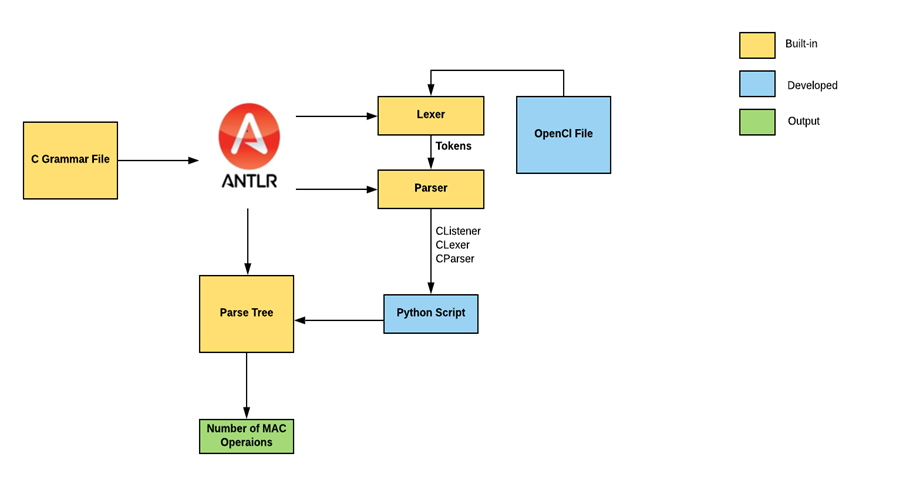
\includegraphics[scale=1.2,width=\textwidth]{img/Antlr4.png}
  \caption{ANTLR4 workflow}
  \label{fig:ANTLR4}
\end{figure}
\pagebreak
\inputminted[breaklines=true]{Python}{img/Antlr4_Python.py}
\captionof{code}{Source Code : OpsCalculator.py\label{code:ANTLR4_Source}}



\begin{code}[!htb]
 \begin{minted}[fontsize=\small]{bash}
[user@fe-1 ~]$ python OpsCalculator.py -kernelfile <path to kernel file> [-v]
\end{minted}
\caption{Command to invoke ANTLR4 based Performance Modeling Tool}
\label{code:ANTLR4Invoke}
\end{code}




\section{Performance Modeling script}
We have used a python script to automate performance modeling for implementations of both GoogLeNet and ResNet. The script considers one kernel at a time, to compute different performance metrics. The metrics are computed according to the specific design of the topology. Thus the given code snippet is for GoogLeNet global memory optimized design and thus needs to be modified for the other designs. The script needs the input and output dimensions of the specific kernel (CNN layer) from the IR along with the execution time from the profiler report in addition to the basic type of kernel such as Conv or Pool. The script is reproduced in Code \ref{code:PerfModel}.

\inputminted[breaklines=true]{Python}{img/PerfModel.py}
\captionof{code}{Source Code : PerformanceModel.py\label{code:PerfModel}}




\section{Python script to generate expected results of CNN Layer}
The functional testing of GoogLeNet and Resnet-50 was carried out by comparing the results at the end of each layer (and/or kernel) with the results generated by TensorFlow running the same models on the same set of inputs. The code used to generate output from TensorFlow has been reproduced in Code \ref{code:TensorFlow}.

\inputminted[breaklines=true]{Python}{img/TensorFlow.py}
\captionof{code}{Source Code : TensorFlow.py\label{code:TensorFlow}}

\section{Python Script to compare Kernel outputs with Tensorflow Outputs}
We can compare the output of our OpenCL implementation with Tensorflow output by using the below code. It generates the Absolute Error between the two outputs.  Python 3 or higher with NumPy 1.16 is necessary to run the code. 

\inputminted[breaklines=true]{Python}{img/abs_error.py}
\captionof{code}{Source Code : abs\_error.py\label{code:abs_error}}

\textbf{Running the script}
For running the script to compare the values, first you should edit the script with file paths and save the script.
\begin{enumerate}
\item Go to line 11 and 13 update the \texttt{tf\_path} and \texttt{tf\_filename} the location to your tensorflow output file.
\item Go to line 16 and 18 update the \texttt{kernel\_path} and \texttt{kernel\_filename} the location to your kernel output file.
\item Run the Python command \\*
          \texttt{python abs\_error.py}
\end{enumerate}

\section{Synthesis Jobs on Notctua Infrastructure}
To execute the CNN topologies the design needed to be synthesized and bitstreams were required to be generated. There are two platform within the $PC^{2}$ infrastructure:
\begin{itemize}
    \item CC- Frontend
    \item Noctua Compute nodes
\end{itemize}
Both of these platforms can be used for synthesizing designs. However, even though the CC-frontend is capable of synthesizing and generating the bitstreams it is not designed for that purpose. For FPGA syntheis there are dedicated compute nodes present in Noctua infrastructure. There are total of 256 compute nodes present which are partitioned into small cluster according to type of synthesis jobs that needs to be carried out.
\newline
For the entirety of the project the compute nodes within \textit{fpgasyn} and \textit{long} partitions were used to generate all the bitstreams.
Noctua cluster uses \raggedright\texttt{Simple Linux Utility for Resource Management (SLURM)} as a workload manager. One has to create a shell script to submit a job to the SLURM workload manager. These are generally called sbatch files. This sheel script contains all the paramaters and the command required to generate a bitstream.
\newpage
\textbf{Batch script for synthesis job}
\begin{minted}{bash}
#!/bin/bash
#SBATCH -N 1
#SBATCH -J unit0
#SBATCH -A hpc-lco-kenter
#SBATCH -p fpgasyn
#SBATCH -t 40:00:00
#SBATCH --mail-type all
#SBATCH --mail-user test@example.com

aoc -v -profile -fp-relaxed -fpc -board=p520_max_sg280l -o /upb/scratch/departments/pc2/groups/pc2-cc-user/custonn2/designs/resnet_units_opv1_bitstream/unit0.aocx unit0.cl -global-ring -duplicate-ring 
\end{minted}
\textbf{Initating a synthesis job}
\begin{enumerate}
    \item Connect to the Noctua Load Balancer using \raggedright\texttt{ssh fe.noctua.pc2.uni-paderborn.de} command
    \item Connect to the compute nodes using \raggedright\texttt{ssh noctua} command
    \item Go the directory where bash script for sbatch is present
    \item Run the sbatch file using \raggedright\texttt{sbatch <filename>.sh} \\*
    \item Type \raggedright\texttt{squeue <username>} to view all the synthesis job
    
\end{enumerate}
%\part{Bibliography, Lists and Appendix}
%\setlength{\emergencystretch}{8em}

\addcontentsline{toc}{chapter}{\listfigurename}
\listoffigures
\addcontentsline{toc}{chapter}{\listequationsname}
\listofequations
\addcontentsline{toc}{chapter}{\listtablename}
\listoftables
\addcontentsline{toc}{chapter}{\listcodename}
\listofcodes
\printbibliography
\clearpage
\end{document}